\chapter{Infinite Derivative Gravity}
\label{chap:2}
\section{Derivation of Action}
Having introduced the concept of infinite derivative gravity theories and some of the progress made in the area, our goal here is to derive the most general, generally covariant infinite derivative action of gravity, with a view to formulating the associated equations of motion. Following this, in Chapter \ref{chap:GF}, we will use the field equations to understand the nature of the modified propagator. 

We begin by inspecting the fluctuations around a given background up to quadratic order in $h$, according to
\[
\label{d0}
g_{\mu\nu}=\eta_{\mu\nu}+h_{\mu\nu}
.\]
For presentation purposes, we have restricted the background metric to that of the Minkowski spacetime as in \cite{Biswas:2011ar}, while the derivation has been repeated in the more general framework of maximally symmetric spacetimes of constant curvature, i.e. Minkowski or (Anti) de Sitter space, in \cite{Biswas:2016egy},\cite{Biswas:2016etb}.  In principle, it should be possible to relax this restriction on the background metric further to any background metric with a well-defined Minkowski limit, with this latter point required to eliminate potentially singular non-local terms. 

As noted in \cite{Biswas:2013kla},\cite{Biswas:2011ar}, the most general, four dimensional, generally covariant metric-tensor-based gravitational action, with a well-defined Minkowski limit, may be expressed in the following generic form
\[
\label{d1}
S=\int d^4 x\sqrt{-g}\left[{\cal P}_0+\sum_i {\cal P}_i \prod_I \left( {\cal O}_{iI}{\cal Q}_{iI}\right)\right]
,\]
where ${\cal P}$ and ${\cal Q}$ are functions of Riemannian curvature and the metric tensor, while the operator ${\cal O}$ is made up, solely, of covariant operators, in accordance with general covariance.

Our goal is to inspect fluctuations around Minkowski space up to quadratic order. To this end, following closely to \cite{Biswas:2016egy},\cite{Biswas:2016etb},\cite{Biswas:2011ar},\cite{Biswas:2005qr}, we may recast \eqref{d1} into the following invariant form
\[
S=S_{EH}+S_{UV},\qquad\mbox{with}\qquad S_{UV}= \int d^4x\sqrt{-g}\left( R_{\mu_1 \nu_1 \lambda_1 \sigma_1}{\cal O}^{\mu_1 \nu_1 \lambda_1 \sigma_1}_{\mu_2 \nu_2 \lambda_2 \sigma_2}R^{\mu_2 \nu_2 \lambda_2 \sigma_2}\right)
\label{d3}
,\]
where $S_{EH}$ is the Einstein-Hilbert action and $S_{UV}$ constitutes the modification of GR in the ultraviolet (UV). The operator ${\cal O}_{\mu_{1}\nu_{1}\lambda_{1}\sigma_{1}}^{\mu_{2}\nu_{2}\lambda_{2}\sigma_{2}}$ represents a general covariant operator, such as the D'Alembertian operator $\Box=g^{\mu\nu}\nabla_{\mu}\nabla_{\nu}$; and the tensor $R_{\mu_{1}\nu_{1}\lambda_{1}\sigma_{1}}$ represents all possible forms of Riemannian curvature, such as the curvature scalar, Ricci Tensor, Riemann and Weyl tensors. It is worth noting that while the generic form \eqref{d3} includes all order of curvature via the commutation relation \eqref{comrel}, we restrict ourselves to a theory that is quadratic in curvature.

Noting that the differential operator ${\cal O}$ contains only the Minkowski metric coupled with covariant derivatives, we may expand the compact form \eqref{d3} to the following
\begin{eqnarray}
S&=&\int d^4x\frac{\sqrt{-g}}{2}\Big[M_P^2R+R F_1(\Box)R+R F_2(\Box)\nabla_{\nu}\nabla_{\mu}R^{\mu\nu}+R_{\mu\nu} F_3(\Box)R^{\mu\nu}\nonumber \\ 
&+&R_{\mu}^{\nu} F_4(\Box)\nabla_{\nu}\nabla_{\lambda}R^{\mu\lambda}+R^{\lambda\sigma} F_5(\Box)\nabla_{\mu}\nabla_{\sigma}\nabla_{\nu}\nabla_{\lambda}R^{\mu\nu}+R F_6(\Box)\nabla_{\mu}\nabla_{\nu}\nabla_{\lambda}\nabla_{\sigma}R^{\mu\nu\lambda\sigma}\nonumber \\ 
&+&R_{\mu\lambda} F_7(\Box)\nabla_{\nu}\nabla_{\sigma}R^{\mu\nu\lambda\sigma}+R_{\lambda}^{\rho} F_8(\Box)\nabla_{\mu}\nabla_{\sigma}\nabla_{\nu}\nabla_{\rho}R^{\mu\nu\lambda\sigma} \nonumber \\ 
& + &R^{\mu_1\nu_1} F_9(\Box)\nabla_{\mu_1}\nabla_{\nu_1}\nabla_{\mu}\nabla_{\nu}\nabla_{\lambda}\nabla_{\sigma}R^{\mu\nu\lambda\sigma}+ R_{\mu\nu\lambda\sigma} F_{10}(\Box)R^{\mu\nu\lambda\sigma} \nonumber \\ 
& + & R^{\rho}{ }_{\mu\nu\lambda} F_{11}(\Box)\nabla_{\rho}\nabla_{\sigma}R^{\mu\nu\lambda\sigma}+ R_{\mu\rho_1 \nu\sigma_1} F_{12}(\Box)\nabla^{\rho_1}\nabla^{\sigma_1}\nabla_{\rho}\nabla_{\sigma}R^{\mu\rho\nu\sigma}
\nonumber\\ &+&
R_{\mu}^{\;\nu_1\rho_1\sigma_1}F_{13}(\Box)\nabla_{\rho_1}\nabla_{\sigma_1}\nabla_{\nu_1}\nabla_{\nu}\nabla_{\rho}\nabla_{\sigma}R^{\mu\nu\lambda\sigma} \nonumber \\ 
& + & R^{\mu_1\nu_1\rho_1\sigma_1} F_{14}(\Box)\nabla_{\rho_1}\nabla_{\sigma_1}
\nabla_{\nu_1}\nabla_{\mu_1}\nabla_{\mu}\nabla_{\nu}\nabla_{\rho}\nabla_{\sigma}R^{\mu\nu\lambda\sigma}\Big]\,,
\label{d4}
\end{eqnarray} where we have liberally used integration by parts and the functions $F_i$ are defined by
 \[
 \label{Fintro}
 F_i(\Box)=\sum^{\infty}_{n=0}{\tilde f}_{i_n}(\Box/M^2)^n
 .\]
These functions contain all orders of the D'Alembertian operator $\Box=g^{\mu\nu}\nabla_\mu \nabla_\nu$\footnote{Up to quadratic order around Minkowski space, the D'Alembertian will appear in the action only as $\Box=\eta^{\mu\nu}\nabla_\mu \nabla_\nu$}, with each operator modulated by the scale of non-locality $M$ to ensure that these functions are dimensionless. The coefficients ${\tilde f}_{i_n}$, as yet unconstrained, ensure that these are arbitrary infinite derivative functions.

The action \eqref{d4} can be reduced upon noting the antisymmetric properties of the Riemann tensor,
\[
\label{RiemAnti}
R_{(\mu\nu)\rho\sigma}=R_{\mu\nu(\rho\sigma)}=0,
\]
along with the (second) Bianchi identity
\[
\label{Bianchi}
 \nabla_\alpha R^\mu_{\;\nu\beta\gamma}+\nabla_\beta R^\mu_{\;\nu\gamma\alpha}+\nabla_\gamma R^\mu_{\;\nu\alpha\beta}=0
.\]
\pagebreak

\noindent\rule[0.5ex]{\linewidth}{0.25pt} 
\emph{Example:}\\
Consider the terms
\[
RF_{1}(\Box)R+RF_{2}(\Box)\nabla_{\nu}\nabla_{\mu}R^{\mu\nu}+	R_{\mu}^{\nu}F_{4}(\Box)\nabla_{\nu}\nabla_{\lambda}R^{\mu\lambda}
.\]
These can be expressed as the following
\[
\label{2-9}
RF_{1}(\Box)R+\frac{1}{2}RF_{2}(\Box)\Box R+	\frac{1}{2}R_{\mu}^{\nu}F_{4}(\Box)\nabla_{\nu}\nabla^{\mu}R
,\]
by noting the identity $\nabla_{\mu}R^{\mu\nu}=\frac{1}{2}\nabla^{\nu}R$ and subsequently $\nabla_{\nu}\nabla_{\mu}R^{\mu\nu}=\frac{1}{2}\Box R$, which results from a contraction of the Bianchi identity \eqref{Bianchi}. We then perform integration by parts on the final term, to find that \eqref{2-9} develops as follows
\begin{align}
	&=RF_{1}(\Box)R+\frac{1}{2}RF_{2}(\Box)\Box R+\frac{1}{2}\nabla^{\mu}\nabla_{\nu}R_{\mu}^{\nu}F_{4}(\Box)R
	\\&=RF_{1}(\Box)R+\frac{1}{2}RF_{2}(\Box)\Box R+\frac{1}{4}RF_{4}(\Box)\Box R
	\\&\equiv RF_{1}(\Box)R.
\end{align}
In the last step, we have redefined the arbitrary function $F_{1}(\Box)$ to incorporate $F_{2}(\Box)$ and $F_{4}(\Box)$. \\
\noindent\rule[0.5ex]{\linewidth}{0.25pt} 
\\\\
Proceeding in a similar manner, we find that the action reduces to 
\begin{eqnarray} 
S&=&\int d^4x\frac{\sqrt{-g}}{2}\Big[M_P^2 R+R F_1(\Box)R + R_{\mu\nu} F_3(\Box)R^{\mu\nu}
+ R F_6(\Box)\nabla_{\mu}\nabla_{\nu}\nabla_{\lambda}\nabla_{\sigma}R^{\mu\nu\lambda\sigma} \nonumber \\
& + & R_{\mu\nu\lambda\sigma} F_{10}(\Box)R^{\mu\nu\lambda\sigma}  +
R_{\mu}^{\nu_1\rho_1\sigma_1}F_{13}(\Box)\nabla_{\rho_1}\nabla_{\sigma_1}\nabla_{\nu_1}\nabla_{\nu}\nabla_{\rho}\nabla_{\sigma}R^{\mu\nu\lambda\sigma} \nonumber \\ 
& + & R^{\mu_1\nu_1\rho_1\sigma_1} F_{14}(\Box)\nabla_{\rho_1}\nabla_{\sigma_1}
\nabla_{\nu_1}\nabla_{\mu_1}\nabla_{\mu}\nabla_{\nu}\nabla_{\rho}\nabla_{\sigma}R^{\mu\nu\lambda\sigma}\Big]\,.
\label{d5}\end{eqnarray}
A final important reduction comes when one notes that, as we are considering fluctuations around Minkowski space, the covariant derivatives commute freely.\\\\
\noindent\rule[0.5ex]{\linewidth}{0.25pt} 
\\\emph{Example:}
\\Take, for example, the $F_6(\Box)$ term in the above expression. We can decompose this in to two parts, like so
\[
RF_{6}(\Box)\nabla_{\mu}\nabla_{\nu}\nabla_{\lambda}\nabla_{\sigma}R^{\mu\nu\lambda\sigma}=\frac{1}{2}RF_{6}(\Box)\nabla_{\mu}\nabla_{\nu}\nabla_{\lambda}\nabla_{\sigma}R^{\mu\nu\lambda\sigma}+\frac{1}{2}RF_{6}(\Box)\nabla_{\mu}\nabla_{\nu}\nabla_{\lambda}\nabla_{\sigma}R^{\mu\nu\lambda\sigma}
.\]
We then commute one pair of derivatives in the first term to find
\[
RF_{6}(\Box)\nabla_{\mu}\nabla_{\nu}\nabla_{\lambda}\nabla_{\sigma}R^{\mu\nu\lambda\sigma}=\frac{1}{2}RF_{6}(\Box)\nabla_{\nu}\nabla_{\mu}\nabla_{\lambda}\nabla_{\sigma}R^{\mu\nu\lambda\sigma}+\frac{1}{2}RF_{6}(\Box)\nabla_{\mu}\nabla_{\nu}\nabla_{\lambda}\nabla_{\sigma}R^{\mu\nu\lambda\sigma}.
\]
Relabelling the indices gives
\[
RF_{6}(\Box)\nabla_{\mu}\nabla_{\nu}\nabla_{\lambda}\nabla_{\sigma}R^{\mu\nu\lambda\sigma}=RF_{6}(\Box)\nabla_{\mu}\nabla_{\nu}\nabla_{\lambda}\nabla_{\sigma}R^{(\mu\nu)\lambda\sigma}=0
,\]
which vanishes due to the antisymmetric properties of the Riemann tensor, \eqref{RiemAnti}.
\noindent\rule[0.5ex]{\linewidth}{0.25pt}
\\\\
Taking this into account, we can now  express the general form of the modified action as follows
\[ \label{f_action}
S=\int d^4x\frac{\sqrt{-g}}{2}\left[M_P^2R+R F_1(\Box)R
+R_{\mu\nu} F_3(\Box)R^{\mu\nu}
+R_{\mu\nu\lambda\sigma} F_{10}(\Box)R^{\mu\nu\lambda\sigma}\right]\,.
\]
We complete the derivation of the most general, generally covariant action of gravity that is quadratic in curvature with a little bookkeeping. First of all, it is preferable to replace the Riemann tensor in the gravitational action with the Weyl tensor, which is defined by
\[
\label{weyl}
C_{\;\alpha\nu\beta}^{\mu}\equiv R_{\;\alpha\nu\beta}^{\mu}-\frac{1}{2}(\delta_{\nu}^{
\mu}R_{\alpha\beta}-\delta_{\beta}^{\mu}R_{\alpha\nu}+R_{\nu}^{\mu}g_{
\alpha\beta}-R_{\beta}^{\mu}g_{\alpha\nu})+\frac{R}{6}(\delta_{\nu}^{\mu}g_{
\alpha\beta}-\delta_{\beta}^{\mu}g_{\alpha\nu})
.\]
This is because the Weyl tensor vanishes precisely in a conformally-flat background, making calculations less cumbersome in, for example, a cosmological Friedmann-Robertson-Walker (FRW) setting. This substitution does not represent any fundamental change to the theory as any change arising from reformulating the above action in terms of the Weyl tensor is absorbed by the arbitrary coefficient ${\tilde f}_{i_n}$ contained within the infinite derivative functions \eqref{Fintro}. In acknowledgement of this minor change, we now rename the infinite derivative functions, like so
 \[
 \label{Fcurly}
 {\cal F}_i(\Box)=\sum^{\infty}_{n=0}f_{i_n}(\Box/M^2)^n
 ,\]
while also renaming the indices for presentation purposes. Finally, we introduce a dimensionless `counting tool' $\lambda$ which offers a straightforward limit $\lambda\rightarrow 0$ to return the theory to that of GR. Taking this into account, we now arrive at the final form of the modified action
\[ \label{action}
S=\int d^4x\frac{\sqrt{-g}}{2}\left[M_P^2R+ \lambda R{\cal F}_1(\Box)R
+\lambda R_{\mu\nu} {\cal F}_2(\Box)R^{\mu\nu}
+\lambda C_{\mu\nu\lambda\sigma} {\cal F}_{3}(\Box)C^{\mu\nu\lambda\sigma}\right]\,.
\]
%\section{Modified Gravitational Action}
%A generic gravitational action that has been modified in the ultraviolet may be expressed as the summation of the Einstein-Hilbert action of General Relativity and an action describing the UV modification
%\begin{equation}
%\label{EHaction}
%S=S^{EH}+S^{UV},
%\end{equation}
%where
%\bg
%S^{EH}=\frac{M_{P}^{2}}{2}\int d^{4}x\sqrt{-g}R,
% \en
%in 4-dimensions. A central tenet of General Relativity is the principle of general covariance, which insists that each term making up a gravitational action will transform in a coordinate-independent way. The principle was first struck upon by Einstein when formulating the theory of special relativity, where it was purported that physical laws will remain consistent in all inertial frames. Furthermore, the universal nature of the tensor transformation law offered a simple means of rendering physical equations generally covariant, in that they could be expressed in terms of tensors. This reformulation of gravity in terms of tensors - with the graviton represented by a type spin-$(2,0)$ metric tensor - allowed for a gravitational theory to be described by curvature alone. This proved to be the cornerstone of General Relativity and made remarkable predictions  in terms of gravitational waves, red-shifting, etc., which would later be verified (Refs) and still a source of fascination and intrigue a century later (Carroll, Wald, Ferreira). However, as mentioned in the introduction, pure GR is beset my some major shortcomings, which we intend to address by modifying the Einstein-Hilbert action. Restricting ourselves to gravitational theories that are quadratic in curvature, we may then express the most general form of the $4$-dimensional, modified action $S^{UV}$
%  that is generally covariant
%\bg
%S^{UV}=R^{\mu_{1}\nu_{1}\lambda_{1}\sigma_{1}}{\cal O}_{\mu_{1}\nu_{1}\lambda_{1}\sigma_{1}}^{\mu_{2}\nu_{2}\lambda_{2}\sigma_{2}}R_{\mu_{2}\nu_{2}\lambda_{2}\sigma_{2}}.
% \en
%Here, the operator ${\cal O}_{\mu_{1}\nu_{1}\lambda_{1}\sigma_{1}}^{\mu_{2}\nu_{2}\lambda_{2}\sigma_{2}}$ represents a general covariant operator, such as the D'Alembertian operator $\Box=g^{\mu\nu}\nabla_{\mu}\nabla_{\nu}$; and the tensor $R^{\mu_{1}\nu_{1}\lambda_{1}\sigma_{1}}$ describes all possible forms of curvature, such as the curvature scalar, Ricci Tensor, Riemann and Weyl tensors. A large volume of work in terms of modified gravity has been concentrated on studying \emph{finite} higher-derivative theories - for instance, $f(R)$ theories of gravity, where the curvature scalar of the EH action \eqref{EHaction} is replaced with an arbitrary function $f$ acting on the curvature
%\bg
%S=\frac{M_P^2}{2}\int d^4 x \sqrt{-g}f(R);
%\en
%or, indeed "Fourth Order Gravity", defined by the Lagrangian
%\bg
%\label{4thorder}
%{\cal L}\sim R+f_1 R^2+f_2 R_{\mu\nu} R^{\mu\nu}+f_3 R^{\mu\nu\lambda\sigma}_{\mu\nu\lambda\sigma},
%\en
%where a particular choice of the coefficients $f_i$ returns the famous Gauss-Bonnet action. The above action yields four derivatives - a feature which confers its name - and has been studied extensively by Stelle (Stelle Refs!). Stelle found that that fourth order gravity is renormalizable, in that the associated modified graviton propagator displays no divergences at 1-loop and beyond. However, this comes at the expense of the ``Weyl" ghost in the tensor component of the modified propagator, placing any predictions from this model on shaky ground.
%The aforementioned modified gravity models are local in nature in that the retain the principle of locality. The principle states that a particle is only directly influenced by its immediate surroundings with such an influence mediated by a field of some sort.
%-introduce concept of non-locality
%-non-locality and the holographic principle
%-non-locality and quantum gravity
%-derivation of non-local action
%
%\bg
%\label{action}
%S=\int d^{4}x\frac{\sqrt{-g}}{2}\left[M_{P}^{2}R+\lambda R{\cal F}_{1}(\Box)R+\lambda R^{\mu\nu}{\cal F}_{2}(\Box)R_{\mu\nu}+\lambda C^{\mu\nu\lambda\sigma}{\cal F}_{3}(\Box)C_{\mu\nu\lambda\sigma}\right]
% \en
\section{Equations of Motion}
Having attained the most general, generally covariant, infinite derivative action of gravity that is quadratic in curvature, the next step is to compute the field equations -- a highly non-trivial task. We begin with an overview of the methods involved, largely based upon \cite{Biswas:2013cha}, before delving into the full technical derivations.
\subsection{General Methodology}
\subsubsection*{Single $\Box$}
In order to illustrate the methods involved in deriving the field equations for the action \eqref{action}, we begin with a simple example, by way of the action,
\bg
S_s = \int d^4 x \sqrt{-g} R\Box R
,\en
where $R$ denotes the curvature scalar. Varying this, gives
\[
\label{varyss}
\delta S_{s}=\int d^{4}x\sqrt{-g}\biggl(\frac{h}{2}R\Box R+\delta R\Box R+R\delta(\Box R)\biggr),
 \]
where we are considering the variation
\[
g_{\mu\nu}\rightarrow g_{\mu\nu}+\delta g_{\mu\nu}
\]
and have defined
\bg
\delta g_{\mu\nu} \equiv h_{\mu\nu}, \mbox{ such that } \delta g^{\mu\nu}=-h^{\mu\nu}
.\footnote{Note: This second identity ($\delta g^{\mu\nu}=-h^{\mu\nu}$) follows from the first ($\delta g_{\mu\nu}\equiv h_{\mu\nu}$), along with the invariance of the Kronecker delta. 
\begin{align*}
\delta_{\nu}^{\mu}	&=g^{\mu\sigma}g_{\sigma\nu}\rightarrow(g^{\mu\sigma}+\delta g^{\mu\sigma})(g_{\sigma\nu}+\delta g_{\sigma\nu})
	=\delta_{\nu}^{\mu}+g^{\mu\sigma}\delta g_{\sigma\nu}+\delta g^{\mu\sigma}g_{\sigma\nu}+{\cal O}(h^{2}),
\end{align*}
which implies that
\[
g^{\mu\sigma}h_{\sigma\nu}=-\delta g^{\mu\sigma}g_{\sigma\nu}.
\]
Act $g^{\nu\tau}$ to both sides to find
\[
h^{\mu\tau}=-\delta g^{\mu\tau}.
\]
}
\en 
One can then compute the variation of the determinant of the metric, which gives
\[
\label{deltasqrt}
\delta\sqrt{-g}=\frac{1}{2}\sqrt{-g}h
,\]
where $h\equiv h^\mu_\mu$~\cite{Veltman:1975vx}. We then note that the D'Alembertian operator $\Box$ contains within it a metric and must therefore be subjected to variation. Upon integration by parts, we may express \eqref{varyss} in the following form
\[
\label{Christoffelh2}
\delta S_{s}=\int d^{4}x\sqrt{-g}\biggl(\frac{h}{2}R\Box R+2\delta R\Box R+R\delta(\Box)R\biggr)
. \]
We will deal with the tricky final term in due course. Firstly, however, we apply the variational principle in order to compute the variation of any relevant curvatures. Upon inspection of the definition of the Christoffel symbol, \eqref{Christoffel}, we find the variation to be of the form
\bg
\label{variedChris}
\delta\Gamma_{\mu\nu}^{\lambda}=\frac{1}{2}\left(\nabla_{\mu}h_{\nu}^{\lambda}+\nabla_{\nu}h_{\mu}^{\lambda}-\nabla^{\lambda}h_{\mu\nu}\right)
. \en
Similarly, variation of the curvature terms, found in \ref{sec:AppCurv}, give
\bg
\nn
\delta R^{\lambda}{ }_{\mu\sigma\nu}=\nabla_{\sigma}\delta\Gamma_{\mu\nu}^{\lambda}-\nabla_{\nu}\delta\Gamma_{\mu\sigma}^{\lambda}
\en 
\bg
\nn
\delta R_{\mu\nu}=\nabla_{\lambda}\delta\Gamma_{\mu\nu}^{\lambda}-\nabla_{\nu}\delta\Gamma_{\mu\lambda}^{\lambda}
 \en
\bg
\delta R=-h^{\mu\nu}R_{\mu\nu}+g^{\mu\nu}\delta R_{\mu\nu}
. \en
Substitution of the above varied Christoffel symbol \eqref{Christoffelh2} allows us to represent the varied curvature in terms of the perturbed metric tensor $h_{\mu\nu}$:
\[
\delta R^{\lambda}{ }_{\mu\sigma\nu}=\frac{1}{2}\left(\nabla_{\sigma}\nabla_{\mu}h_{\;\nu}^{\lambda}-\nabla_{\sigma}\nabla^{\lambda}h_{\mu\nu}-\nabla_{\nu}\nabla_{\mu}h_{\;\sigma}^{\lambda}+\nabla_{\nu}\nabla^{\lambda}h_{\mu\sigma}\right)
\nn \]
\[
\delta R_{\mu\nu}=\frac{1}{2}\left(\nabla_{\lambda}\nabla_{\mu}h_{\nu}^{\lambda}+\nabla_{\lambda}\nabla_{\nu}h_{\mu}^{\lambda}-\Box h_{\mu\nu}-\nabla_{\nu}\nabla_{\mu}h\right)
 \nn\]
\[
\label{varyids}
\delta R=-R^{\mu\nu}h_{\mu\nu}+\nabla_{\lambda}\nabla^{\sigma}h_{\sigma}^{\lambda}-\Box h
\] 
Identities of this type are well known. What is less clear, however, is the computation of $\delta(\Box)R$, which we shall detail below.
\subsubsection*{Computing $\delta(\Box)R$}
By expanding out the components of the D'Alembertian, we have
\bg
\label{deltaboxR0}
\delta(\Box)R=\delta(g^{\mu\nu}\nabla_{\mu}\nabla_{\nu})R=-h^{\mu\nu}\nabla_{\mu}\nabla_{\nu}R+g^{\mu\nu}\delta(\nabla_{\mu})\nabla_{\nu}R+g^{\mu\nu}\nabla_{\mu}\delta(\nabla_{\nu})R
. \en
We find here some terms that involve the variation of the covariant operator, which are not so trivial. However, by varying the tensor $\nabla_\mu\nabla_\nu R$, we may equate these non-trivial terms with the variation of ordinary tensors, like so
\bg
\delta(\nabla_{\mu})\partial_{\nu}R+\nabla_{\mu}\delta(\nabla_{\nu})R=\delta(\nabla_{\mu}\nabla_{\nu}R)-\nabla_{\mu}\nabla_{\nu}\delta R.
\en
Next, we compute the terms on the right hand side by expanding out the covariant derivative so that, after some cancellation, we get an identity in terms of the Christoffel symbol
\bg
\delta(\nabla_{\mu})\partial_{\nu}R+\nabla_{\mu}\delta(\nabla_{\nu})R=-\delta\Gamma_{\mu\nu}^{\kappa}\partial_{\kappa}R
.\en
We briefly note that the simplicity of this identity is due to the scalar nature of the curvature involved. Tensors of higher order, such as the Ricci or Riemann tensor, will result in additional terms. Upon substitution into  \eqref{deltaboxR0} in conjunction with the variation of the Christoffel stated previously in \eqref{varyids}, we arrive at a vital result in computing the field equations for a non-local action of the type \eqref{action}.
\bg
\label{deltaboxR}
\delta(\Box)R=-h^{\mu\nu}\nabla_{\mu}\nabla_{\nu}R-\nabla^{\sigma}h_{\sigma}^{\kappa}\partial_{\kappa}R+\frac{1}{2}\partial^{\kappa}h\partial_{\kappa}R
. \en
\subsubsection*{Multiple $\Box$'s}
Crucially, however, in order to derive the field equations for an infinite derivative action such as \eqref{action}, the above mechanism must be generalised to encapsulate an arbitrary number of D'Alembertian operators acting on the curvature. To shed light on this, we consider the action
\bg
\label{actionboxn}
S_{m}=\int d^{4}x\sqrt{-g}R\Box^{n}R.
 \en
Varying with respect to the metric tensor gives
\bg
\delta S_{m}=\int d^{4}x\sqrt{-g}\biggl(\frac{h}{2}R\Box^{n}R+\delta R\Box^{n}R+R\delta(\Box^{n})R+R\Box^{n}\delta R\biggr),
\en 
analogous to \eqref{varyss}. We now turn our attention to the $R\delta(\Box^{n})R$ term. Repeated application of the product rule reveals the following
\begin{align}
R\delta(\Box^{n})R	&=	R\Box\delta(\Box^{n-1})R+R\delta(\Box)\Box^{n-1} R
\nn\\&	...	
\nn\\&	=\sum_{m=0}^{n-1}	R\Box^{m}\delta(\Box)\Box^{n-m-1}R.
\label{deltaboxn}
 \end{align}
It is then straightforward to substitute \eqref{deltaboxR} into this identity, along with the previously derived varied  curvature terms \eqref{varyids} to reveal the field equations for an action of the type \eqref{actionboxn}.
\subsubsection*{Arbitrary functions of $\Box$}
We may generalise further by considering actions of the type
\bg
S_{F}\sim\int d^{4}x\sqrt{-g}R{\cal F}(\Box)R,
\en 
where ${\cal F}(\Box)$
  is an arbitrary function of D'Alembertian operators of the form 
  \[
  {\cal F}(\Box)\equiv\sum_{n=0}^{\infty}f_{1_{n}}\frac{\Box^{n}}{M^{2n}}.
\]
Here, $f_{1_{n}}$ are arbitrary constants and each non-local operator is modulated by the scale of non-locality, $M$. For such an action, the analogue of \eqref{deltaboxn} is given by
\[
\label{deltaboxf}
R\delta{\cal F}_{1}(\Box)R=\sum_{n=1}^{\infty}\frac{f_{1_{n}}}{M^{2n}}\sum_{m=0}^{n-1}R\Box^{m}\delta(\Box)\Box^{n-m-1}R.
\]
Furthermore, the prescription
\bg
\label{trick}
\int d^4 x\sqrt{-g}\sum_{l}\sum_{m}\Box^{m}A\Box^{l}B=\int d^4 x\sqrt{-g}\sum_{l}\sum_{m}\Box^{l}A\Box^{m}B,
\en 
where $A$ and $B$ are arbitrary tensors, allows us to recast the identity into the following manageable form
\bg
R\delta{\cal F}_{1}(\Box)R=\sum_{n=1}^{\infty}f_{1_{n}}\sum_{m=0}^{n-1}\Box^{m}R\delta(\Box)\Box^{n-m-1}R.
\en 
A final important point is that as $R$
  is a scalar, so too is $\Box^{n-m-1}R$,
  and as such the derived identity for $\delta(\Box)R$
  remains valid for our intentions, where one simply has to substitute $R\rightarrow\Box^{n-m-1}R$
  in \eqref{deltaboxR}. We shall see in the subsequent sections, the central role these observations play in deriving the full field equations for \eqref{action}.
\subsubsection*{Full Action}  
  We are now ready to compute the variation of our action \eqref{action}. For simplicity of presentation, we proceed by decomposing the action into its constituent parts which we denote $S_{0,...,3}$. We define the the gravitational energy momentum tensor as
 \begin{equation}
 T^{\mu\nu}=-\frac{2}{\sqrt{-g}}\frac{\delta S}{\delta g_{\mu\nu}},
 \end{equation}
 where $g\equiv |\det g_{\mu\nu}|$ is the determinant of the metric tensor, and compute the contribution to $T^{\mu\nu}$ for the individual sectors of the action separately.
\subsection{$S_0$}
$S_0$ is nothing more than the Einstein-Hilbert action
\begin{equation}
S_{0}=\frac{1}{2}\int d^{4}x\sqrt{-g}\left(M_P^2R-2\Lambda\right),
  \end{equation}
where, in our formalism, we have taken the cosmological constant $\Lambda$ to be of mass dimension $4$. Varying the action and substituting the identity for the varied curvature scalar \eqref{varyids},  along with \eqref{deltasqrt}, leads to the Einstein equation
\begin{equation}
\begin{aligned} T^{\mu\nu} & =M_P^2 G^{\mu\nu}+g^{\mu\nu}\Lambda\end{aligned}
 \end{equation}
 \subsection{$S_1$}
 The next step is to compute the variation of
\begin{equation}
S_{1}=\frac{1}{2}\int d^{4}x\sqrt{-g}R{\cal F}_{1}(\Box)R\ .
\end{equation}
Varying this and substituting values for $\delta R$ and $\delta \sqrt{-g}$, given in \eqref{varyids} and \eqref{deltasqrt}, respectively, we
find 
\begin{align}
\delta S_{1}&=\frac{1}{2}\int d^{4}x\sqrt{-g}\biggl[\biggl(\frac{1}{2}g^{\mu\nu}R{\cal F}_{1}(\Box)R+2\nabla^{\mu}\nabla^{\nu}{\cal F}_{1}(\Box)R
\nn\\&
-2g^{\mu\nu}\square{\cal F}_{1}(\Box)R-2R^{\mu\nu}{\cal F}_{1}(\Box)R\biggr)h_{\mu\nu}+R\delta{\cal F}_{1}(\Box)R\biggr]
 \end{align}
where we have integrated by parts where appropriate. To calculate the final term, we employ the identity in \eqref{deltaboxf} and substitute the value for $\delta(\Box)R$ given in \eqref{deltaboxR}. We then integrate by parts in order to factor out the perturbed metric $h_{\mu\nu}$. Further terms will simplify by noting the double summation relation given by \eqref{trick}, until we arrive at the energy-momentum tensor contribution, which is given by
\begin{align}
T_{1}^{\mu\nu}&=2G^{\mu\nu}{\cal F}_{1}(\Box)R+\frac{1}{2}g^{\mu\nu}R{\cal F}_{1}(\Box)R-2\left(\nabla^{\mu}\nabla^{\nu}-g^{\mu\nu}\Box\right){\cal F}_{1}(\Box)R
\nn\\&
-\Omega_{1}^{\mu\nu}+\frac{1}{2}g^{\mu\nu}(\Omega_{1\sigma}^{\;\sigma}+\bar{\Omega}_{1})\,,
 \end{align}
where we have defined the symmetric tensors
\begin{equation}
\Omega_{1}^{\alpha\beta}=\sum_{n=1}^{\infty}f_{1_{n}}\sum_{l=0}^{n-1}\nabla^{
\alpha}R^{(l)}\nabla^{\beta}R^{(n-l-1)},\quad\bar{\Omega}_{1}=\sum_{n=1}^{\infty
}f_{1_{n}}\sum_{l=0}^{n-1}R^{(l)}R^{(n-l)},
\end{equation}
and have introduced the notation $\Box^n R\equiv R^{(n)}$.

\subsection{$S_2$}
We now focus on
\[
\label{s2}
S_{2}=\frac{1}{2}\int d^{4}x\sqrt{-g}\left(R^{\mu\nu}{\cal F}_{2}(\Box)R_{\mu\nu}\right)\,.
 \]

Varying the action, we find
\begin{align}
\delta S_{2}	&=\frac{1}{2}\int d^{4}x\biggl[\delta\sqrt{-g}\left(R^{\mu\nu}{\cal F}_{2}(\Box)R_{\mu\nu}\right)+\sqrt{-g}\delta R^{\mu\nu}{\cal F}_{2}(\Box)R_{\mu\nu}
\nn\\&+\sqrt{-g}R^{\mu\nu}{\cal F}_{2}(\Box)\delta R_{\mu\nu}
	+\sqrt{-g}R^{\mu\nu}\delta{\cal F}_{2}(\Box)R_{\mu\nu}\,\biggr].
\end{align}
Careful substitution of the identities found in \ref{sec:Appvary}, accounts for all but the final term:
\begin{align}
\delta S_{2}	&=	\frac{1}{2}\int d^{4}x\sqrt{-g}\biggl[\biggl(\frac{1}{2}g^{\mu\nu}R^{\sigma\tau}{\cal F}_{2}(\Box)R_{\sigma\tau}-2R_{\sigma}^{\nu}{\cal F}_{2}(\Box)R^{\sigma\mu}+2\nabla_{\sigma}\nabla^{\mu}{\cal F}_{2}(\Box)R^{\sigma\nu}
		\nn\\&
		-\square{\cal F}_{2}(\Box)R^{\mu\nu}-g^{\mu\nu}\nabla_{\sigma}\nabla_{\tau}{\cal F}_{2}(\Box)R^{\sigma\tau}\biggl)h_{\mu\nu}+\int d^{4}x\sqrt{-g}R^{\mu\nu}\delta{\cal F}_{2}(\Box)R_{\mu\nu}\biggr].
 \label{varys3}
\end{align}
To compute the final term, we employ the same method outlined in the general methodology section, albeit with an added degree of difficulty. Here, we reiterate the main steps. In terms of the Ricci tensor, the analogous identity of (\ref{deltaboxn}) is arrived at by identical means,
\begin{equation}
\label{deltaFRuv}
R^{\mu\nu}\delta{\cal F}_2(\Box)R_{\mu\nu}=\sum_{m=0}^{
n-1 }
\sum_{n=1}^{\infty}f_{2_n}R^{\mu\nu(m)}\delta(\square)R_{\mu\nu}^{(n-m-1)}\,.
\end{equation}
Of vital importance, however, is the form of $\delta(\Box)R_{\mu\nu}$. We expand out the components of the D'Alembertian operator, in the same manner as in the scalar case, before taking the variation
\begin{equation}
\label{deltaboxRuv1}
\delta(\Box)R_{\mu\nu}=\delta(g^{\sigma\tau}\nabla_\sigma \nabla_\tau)R_{\mu\nu}=h^{\sigma\tau}\nabla_\sigma \nabla_\tau R_{\mu\nu}+g^{\sigma\tau}\delta(\nabla_\sigma)\nabla_\tau R_{\mu\nu}+g^{\sigma\tau}\nabla_\sigma \delta(\nabla_\tau)R_{\mu\nu}.
\end{equation}
%where $S_{\mu\nu}$ is an arbitrary ${0,2}$-tensor, representative of the Ricci tensor $R_{\mu\nu}$ or indeed any number of D'Alembertian operators acting upon the Ricci tensor $R_{\mu\nu}^{(n-m-1)}$.
As in the scalar case, \eqref{deltaboxR}, we compare $\delta(\nabla_\tau R_{\mu\nu})$ with $\nabla_\tau \delta R_{\mu\nu}$ to find
\begin{equation}
\delta(\nabla_{\tau})R_{\mu\nu}=-\delta\Gamma_{\tau\mu}^{\kappa}R_{\kappa\nu}-\delta\Gamma_{\tau\nu}^{\kappa}R_{\mu\kappa}
 \nn 
\end{equation}
\begin{equation}
\label{deltanablaRuv}
\delta(\nabla_{\sigma})\nabla_{\tau}R_{\mu\nu}=-\delta\Gamma_{\tau\mu}^{\kappa}\nabla_{\tau}R_{\kappa\nu}-\delta\Gamma_{\tau\nu}^{\kappa}\nabla_{\tau}R_{\mu\kappa}-\delta\Gamma_{\tau\nu}^{\kappa}\nabla_{\kappa}R_{\mu\nu}.
\end{equation}
At this point, in order to keep track of the indices, it is convenient to rewrite the perturbed Christoffel symbol \eqref{variedChris}, like so
\begin{equation}
\label{Christoffelhab}
\delta\Gamma_{\mu\nu}^{\lambda}=\frac{1}{2}\left(\delta_{\nu}^{\beta}g^{\alpha\lambda}\nabla_{\mu}+\delta_{\mu}^{\beta}g^{\alpha\lambda}\nabla_{\nu}-\delta_{\mu}^{\alpha}\delta_{\nu}^{\beta}\nabla^{\lambda}\right)h_{\alpha\beta}.
 \end{equation}
 We then substitute this into \eqref{deltanablaRuv} and in turn \eqref{deltaboxRuv1} to find the relevant identity:
 \begin{align}
 \label{deltaBoxSuv}
 \delta(\square)R_{\mu\nu}	&=	\biggl[-\nabla^{\alpha}\nabla^{\beta}R_{\mu\nu}-\nabla^{\alpha}R_{\mu\nu}\nabla^{\beta}+\frac{1}{2}g^{\alpha\beta}\nabla_{\sigma}R_{\mu\nu}\nabla^{\sigma}
		\nn\\&
		-\frac{1}{2}\delta_{(\mu}^{\beta}R_{\;\nu)}^{\alpha}\Box+\frac{1}{2}\delta_{(\mu}^{\beta}R_{\tau\nu)}\nabla^{\alpha}\nabla^{\tau}-\frac{1}{2}R_{\;(\nu}^{\alpha}\nabla^{\beta}\nabla_{\mu)}
		\nn\\&
		-\nabla^{\beta}R_{\;(\nu}^{\alpha}\nabla_{\mu)}-\delta_{(\mu}^{\beta}\nabla^{\lambda}R_{\;\nu)}^{\alpha}\nabla_{\lambda}+\delta_{(\mu}^{\beta}\nabla^{\alpha}R_{\tau\nu)}\nabla^{\tau}\biggr]h_{\alpha\beta}.
 \end{align}
Having established the form of $\delta(\square)R_{\mu\nu}$, we are now in a position to tame the troublesome term \eqref{deltaFRuv} into something manageable, like so
\begin{equation}
\int d^{4}x\sqrt{-g}R^{\mu\nu}\delta{\cal F}_{2}(\Box)R_{\mu\nu}=\int d^{4}x\sqrt{-g}\left(\Omega_{2}^{\mu\nu}-\frac{1}{2}g^{\mu\nu}(\Omega_{2\sigma}^{\;\sigma}+\bar{\Omega}_{2})+2\Delta_{2}^{\mu\nu}\right)h_{\mu\nu}\,.
 \end{equation}
where we have defined the following symmetric tensors,
\begin{equation}
\nn
\Omega_{2}^{\mu\nu}=\sum_{n=1}^{\infty}f_{2_{n}}\sum_{l=0}^{n-1}\nabla^{\mu}R_{\tau}^{\sigma(l)}\nabla^{\nu}R_{\sigma}^{\tau(n-l-1)},\quad\bar{\Omega}_{2}=\sum_{n=1}^{\infty}f_{2_{n}}\sum_{l=0}^{n-1}R_{\tau}^{\sigma(l)}R_{\sigma}^{\tau(n-l)}\,,
\end{equation}
\begin{equation}
\Delta_{2}^{\mu\nu}=\sum_{n=1}^{\infty}f_{2_{n}}\sum_{l=0}^{n-1}\nabla_{\tau}\left(R_{\;\sigma}^{\tau(l)}\nabla^{\mu}R^{\nu\sigma(n-l-1)}-\nabla^{\mu}R_{\;\sigma}^{\tau(l)}R^{\nu\sigma(n-l-1)}\right),
\end{equation}
This, combined with (\ref{varys3}), gives us the contribution of the Ricci tensor terms to the energy-momentum tensor
\begin{align}
T_{2}^{\mu\nu}	&=	-\frac{1}{2}g^{\mu\nu}R^{\sigma\tau}{\cal F}_{2}(\Box)R_{\sigma\tau}+2R_{\sigma}^{\nu}{\cal F}_{2}(\Box)R^{\sigma\mu}-2\nabla_{\sigma}\nabla^{\mu}{\cal F}_{2}(\Box)R^{\sigma\nu}
		\nn\\&+\square{\cal F}_{2}(\Box)R^{\mu\nu}+g^{\mu\nu}\nabla_{\sigma}\nabla_{\tau}{\cal F}_{2}(\Box)R^{\sigma\tau}-\Omega_{2}^{\mu\nu}+\frac{1}{2}g^{\mu\nu}(\Omega_{2\sigma}^{\;\sigma}+\bar{\Omega}_{2})-2\Delta_{2}^{\mu\nu},
 \label{P2}
\end{align}
\subsection{$S_3$}
Finally we focus on the terms involving the Weyl tensors. We proceed in much the same manner as the previous case, with a further layer of complexity due to the number of indices involved. The action we wish to vary is given by
\[
S_{3}=\frac{1}{2}\int d^{4}x\sqrt{-g}C^{\mu\nu\lambda\sigma}{\cal
F}_{3}(\Box)C_{\mu\nu\lambda\sigma},
\]
where the Weyl tensor is defined by
\[
\label{weyl}
C^{\mu}{ }_{\alpha\nu\beta}\equiv R^{\mu}{ }_{\alpha\nu\beta}-\frac{1}{2}(\delta_{\nu}^{
\mu}R_{\alpha\beta}-\delta_{\beta}^{\mu}R_{\alpha\nu}+R_{\nu}^{\mu}g_{
\alpha\beta}-R_{\beta}^{\mu}g_{\alpha\nu})+\frac{R}{6}(\delta_{\nu}^{\mu}g_{
\alpha\beta}-\delta_{\beta}^{\mu}g_{\alpha\nu})
.\]
Varying the action we find
\[\delta S_{3}=\frac{1}{2}\sqrt{-g}\int d^{4}x\biggl[\frac{1}{2}g^{\alpha\beta}h_{\alpha\beta}C^{\mu\nu\lambda\sigma}{\cal F}_{3}(\Box)C_{\mu\nu\lambda\sigma}+\delta\left(C^{\mu\nu\lambda\sigma}{\cal F}_{3}(\Box)C_{\mu\nu\lambda\sigma}\right)\biggr].
 \]
Once again, we intend to arrange the expression in terms of the metric tensor $h_{\alpha\beta}$. The second term develops as follows
\begin{align}
\delta&\left(C^{\mu\nu\lambda\sigma}{\cal F}_{3}(\Box)C_{\mu\nu\lambda\sigma}\right)	=	\delta C^{\mu\nu\lambda\sigma}{\cal F}_{3}(\Box)C_{\mu\nu\lambda\sigma}+C^{\mu\nu\lambda\sigma}\delta({\cal F}_{3}(\Box)C_{\mu\nu\lambda\sigma})
	\nn\\&=	\delta(g^{\nu\rho}g^{\phi\lambda}g^{\sigma\psi}C^{\mu}{ }_{\rho\phi\psi}){\cal F}_{3}(\Box)C_{\mu\nu\lambda\sigma}+C^{\mu\nu\lambda\sigma}\delta({\cal F}_{3}(\Box)g_{\mu\rho}C^{\rho}{ }_{\nu\lambda\sigma})
	\nn\\&=	-4h^{\nu\rho}C^{\mu}{ }_{\rho\phi\psi}{\cal F}_{3}(\Box)C_{\mu\nu}{ }{ }^{\phi\psi}+\delta C^{\mu}{ }_{\rho\phi\psi}{\cal F}_{3}(\Box)C_{\mu}{ }^{\rho\phi\psi}+C_{\rho}{ }^{\nu\lambda\sigma}\delta({\cal F}_{3}(\Box)C^{\rho}{ }_{\nu\lambda\sigma})
	\nn\\&=	-4h^{\alpha\beta}C_{\beta\mu\nu\lambda}^{\;}{\cal F}_{3}(\Box)C_{\alpha}{ }^{\mu\nu\lambda}+2\delta C^{\mu}{ }_{\nu\lambda\sigma}{\cal F}_{3}(\Box)C_{\mu}{ }^{\nu\lambda\sigma}+C_{\mu}{ }^{\nu\lambda\sigma}\delta{\cal F}_{3}(\Box)C^{\mu}{ }_{\nu\lambda\sigma}
  \end{align}
Next, using the definition of the Weyl tensor (\eqref{weyl}), we note that
\[
\delta C^{\mu}{ }_{\nu\lambda\sigma}{\cal F}_{3}(\Box)C_{\mu}{ }^{\nu\lambda\sigma}=\left(\delta R^{\mu}{ }_{\nu\lambda\sigma}-\frac{1}{2}(R_{\lambda}^{\mu}h_{\nu\sigma}-R_{\sigma}^{\mu}h_{\nu\lambda})\right){\cal F}_{3}(\Box)C_{\mu}{ }^{\nu\lambda\sigma}.
\]
Here, we have used the essential property 
\[
C^{\mu}{ }_{\nu\mu\lambda}=0
,\]
which is due to the fact that the Weyl tensor is the traceless component of the Riemann tensor. We then reformulate the variation of the Riemann tensor \eqref{varyids} like so
\[
\delta R^{\lambda}{ }_{\mu\sigma\nu}=\frac{1}{2}\left(g^{\alpha\lambda}\delta_{\nu}^{\beta}\nabla_{\sigma}\nabla_{\mu}-\delta_{\mu}^{\alpha}\delta_{\nu}^{\beta}\nabla_{\sigma}\nabla^{\lambda}-g^{\alpha\lambda}\delta_{\sigma}^{\beta}\nabla_{\nu}\nabla_{\mu}+\delta_{\mu}^{\alpha}\delta_{\sigma}^{\beta}\nabla_{\nu}\nabla^{\lambda}\right)h_{\alpha\beta}
, \]
and substitute to find
\[
2\delta C^{\mu}{ }_{\nu\lambda\sigma}{\cal F}_{3}(\Box)C_{\mu}{ }^{\nu\lambda\sigma}	=	-2\left(R_{\nu}^{\mu}+2\nabla_{\nu}\nabla^{\mu}\right){\cal F}_{3}(\Box)C_{\mu}{ }^{\alpha\nu\beta}h_{\alpha\beta},
  \]
where we have integrated by parts where appropriate. The variation of the action, thus far, is then given by
\begin{align}
\delta S_{3}	&=	\frac{1}{2}\int d^{4}x\sqrt{-g}\biggl[\biggl(\frac{1}{2}g^{\alpha\beta}C^{\mu\nu\lambda\sigma}{\cal F}_{3}(\Box)C_{\mu\nu\lambda\sigma}-4C_{\;\mu\nu\lambda}^{\beta}{\cal F}_{3}(\Box)C^{\alpha\mu\nu\lambda}
\nn\\&-2\left(R_{\mu\nu}+2\nabla_{\nu}\nabla_{\mu}\right){\cal F}_{3}(\Box)C^{\mu\alpha\nu\beta}\biggr)h_{\alpha\beta}+\frac{1}{2}C_{\mu}{ }^{\nu\lambda\sigma}\delta{\cal F}_{3}(\Box)C^{\mu}{ }_{\nu\lambda\sigma}\biggr].
 \end{align}
To compute the final term, we proceed as in the previous cases to derive $\delta(\Box)$ acting upon the Weyl tensor:
\begin{align}
\delta(\Box)C_{\mu\nu\lambda\sigma}	&=	\biggl[-\nabla^{\alpha}\nabla^{\beta}C_{\mu\nu\lambda\sigma}-\nabla^{\alpha}C_{\mu\nu\lambda\sigma}\nabla^{\beta}+\frac{1}{2}g^{\alpha\beta}\nabla_{\tau}C_{\mu\nu\lambda\sigma}\nabla^{\tau}
		\nn\\&-\frac{1}{2}C^{\alpha}{ }_{\nu\lambda\sigma}\nabla^{\beta}\nabla_{\mu}+\frac{1}{2}C^{\alpha}{ }_{\mu\lambda\sigma}\nabla^{\beta}\nabla_{\nu}+\frac{1}{2}C^{\alpha}{ }_{\mu\nu\sigma}\nabla^{\beta}\nabla_{\lambda}+\frac{1}{2}C^{\alpha}{ }_{\lambda\mu\nu}\nabla^{\beta}\nabla_{\sigma}
		\nn\\&-\nabla^{\beta}C^{\alpha}{ }_{\nu\lambda\sigma}\nabla_{\mu}+\nabla^{\beta}C^{\alpha}{ }_{\mu\lambda\sigma}\nabla_{\nu}-\nabla^{\beta}C^{\alpha}{ }_{\sigma\mu\nu}\nabla_{\lambda}+\nabla^{\beta}C^{\alpha}{ }_{\lambda\mu\nu}\nabla_{\sigma}\biggr]h_{\alpha\beta}.
 \end{align}
From this, we deduce
\[
\int
d^{4}x\sqrt{-g} C^{\mu\nu\lambda\sigma}\delta{\cal
F}_{3}(\Box)C_{\mu\nu\lambda\sigma}=\int
d^{4}x\sqrt{-g}\left(\Omega_{3}^{\alpha\beta}-\frac{1}{2}g^{
\alpha\beta}(\Omega_{3\gamma}^{\;\gamma}+\bar{\Omega}_{3})+4\Delta_{3}^{
\alpha\beta}\right)h_{\alpha\beta}\,,
\]
by defining
\[
\Omega_{3}^{\alpha\beta}=\sum_{n=1}^{\infty}f_{3_{n}}\sum_{l=0}^{n-1}\nabla^{\alpha}C_{\;\nu\lambda\sigma}^{\mu(l)}\nabla^{\beta}C_{\mu}^{\;\nu\lambda\sigma(n-l-1)},\quad\bar{\Omega}_{3}=\sum_{n=1}^{\infty}f_{3_{n}}\sum_{l=0}^{n-1}C_{\;\nu\lambda\sigma}^{\mu(l)}C_{\mu}^{\;\nu\lambda\sigma(n-l)}\,,
\nn \]
\[
 \Delta_{3}^{\alpha\beta}=\sum_{n=1}^{\infty}f_{3_{n}}\sum_{l=0}^{n-1}\nabla_{\nu}\left(C_{\;\;\;\sigma\mu}^{\lambda\nu(l)}\nabla^{\alpha}C_{\lambda}^{\;\beta\sigma\mu(n-l-1)}-\nabla^{\alpha}C_{\;\;\;\sigma\mu}^{\lambda\nu\;\;(l)}C_{\lambda}^{\;\beta\sigma\mu(n-l-1)}\right).
 \]
As such, the contribution to the energy-momentum tensor is then
\begin{align}
T_{3}^{\mu\nu}	&=	-\frac{1}{2}g^{\mu\nu}C^{\sigma\tau\lambda\rho}{\cal F}_{3}(\Box)C_{\sigma\tau\lambda\rho}+4C_{\;\sigma\tau\lambda}^{\nu}{\cal F}_{3}(\Box)C^{\mu\sigma\tau\lambda}+2\left(R_{\sigma\tau}+2\nabla_{\tau}\nabla_{\sigma}\right){\cal F}_{3}(\Box)C^{\sigma\mu\tau\nu}
		\nn\\&-\Omega_{3}^{\mu\nu}+\frac{1}{2}g^{\mu\nu}(\Omega_{3\gamma}^{\;\gamma}+\bar{\Omega}_{3})-4\Delta_{3}^{\mu\nu},
   \end{align}
   where we have reintroduced the original $_\mu,_\nu$ notation by relabelling the indices.
\subsection{The Complete Field Equations}
We are now in a position to state the full equations of motion for the action $S$ in
(\ref{action}) as a combination of $S_0,\;S_1,\;S_2$ and $S_3$ derived in the previous sections.
\begin{align}
\label{eomfull}
T_{\nu}^{\mu}	&=	M_{P}^{2}G_{\nu}^{\mu}+\delta_{\nu}^{\mu}\Lambda+2\lambda G_{\nu}^{\mu}{\cal F}_{1}(\Box)R+\frac{\lambda}{2}\delta_{\nu}^{\mu}R{\cal F}_{1}(\Box)R-2\lambda\left(\nabla^{\mu}\partial_{\nu}-\delta_{\nu}^{\mu}\square\right){\cal F}_{1}(\Box)R
		\nn\\&+2\lambda R_{\sigma}^{\mu}{\cal F}_{2}(\Box)R_{\;\nu}^{\sigma}-\frac{\lambda}{2}\delta_{\nu}^{\mu}R_{\;\tau}^{\sigma}{\cal F}_{2}(\Box)R_{\;\sigma}^{\tau}-2\lambda\nabla_{\sigma}\nabla_{\nu}{\cal F}_{2}(\Box)R^{\mu\sigma}+\lambda\square{\cal F}_{2}(\Box)R_{\nu}^{\mu}
		\nn\\&+\lambda\delta_{\nu}^{\mu}\nabla_{\sigma}\nabla_{\tau}{\cal F}_{2}(\Box)R^{\sigma\tau}-\frac{\lambda}{2}\delta_{\nu}^{\mu}C^{\sigma\tau\lambda\rho}{\cal F}_{3}(\Box)C_{\sigma\tau\lambda\rho}+4\lambda C_{\;\sigma\tau\lambda}^{\mu}{\cal {\cal F}}_{3}(\square)C_{\nu}^{\;\sigma\tau\lambda}
		\nn\\&-2\lambda\left(R_{\sigma\tau}+2\nabla_{\sigma}\nabla_{\tau}\right){\cal {\cal F}}_{3}(\square)C_{\nu}^{\;\sigma\tau\mu}-\lambda\Omega_{1\nu}^{\mu}+\frac{\lambda}{2}\delta_{\nu}^{\mu}(\Omega_{1\sigma}^{\;\sigma}+\bar{\Omega}_{1})
		\nn\\&-\lambda\Omega_{2\nu}^{\mu}+\frac{\lambda}{2}\delta_{\nu}^{\mu}(\Omega_{2\sigma}^{\sigma}+\bar{\Omega}_{2})-2\lambda\Delta_{2\nu}^{\mu}-\lambda\Omega_{3\nu}^{\mu}+\frac{\lambda}{2}\delta_{\nu}^{\mu}(\Omega_{3\gamma}^{\gamma}+\bar{\Omega}_{3})-4\lambda\Delta_{3\nu}^{\mu},
   \end{align}
where $T^\mu_{\nu}$ is the stress energy tensor for the matter components of the Universe \footnote{We have lowered an index for convenience when analysing perturbations later in the text.} and we restate the symmetric tensors, we defined earlier:
\[\nn
\label{Omegas}
\Omega_{1\nu}^{\mu}=\sum_{n=1}^{\infty}f_{1_{n}}\sum_{l=0}^{n-1}\partial^{\mu}R^{(l)}\partial_{\nu}R^{(n-l-1)},\quad\bar{\Omega}_{1}=\sum_{n=1}^{\infty}f_{1_{n}}\sum_{l=0}^{n-1}R^{(l)}R^{(n-l)},
 \]
\[\nn
\Omega_{2\nu}^{\mu}=\sum_{n=1}^{\infty}f_{2_{n}}\sum_{l=0}^{n-1}\nabla^{\mu}R_{\tau}^{\sigma(l)}\nabla_{\nu}R_{\sigma}^{\tau(n-l-1)},\quad\bar{\Omega}_{2}=\sum_{n=1}^{\infty}f_{2_{n}}\sum_{l=0}^{n-1}R_{\tau}^{\sigma(l)}R_{\sigma}^{\tau(n-l)}\,,
 \]
\[\nn
\Delta_{2\nu}^{\mu}=\sum_{n=1}^{\infty}f_{2_{n}}\sum_{l=0}^{n-1}\nabla_{\tau}\left(R_{\;\sigma}^{\tau(l)}\nabla^{\mu}R^{\nu\sigma(n-l-1)}-\nabla^{\mu}R_{\;\sigma}^{\tau(l)}R^{\nu\sigma(n-l-1)}\right)\,,
 \]
\[\nn
\Omega_{3\nu}^{\mu}=\sum_{n=1}^{\infty}f_{3_{n}}\sum_{l=0}^{n-1}\nabla^{\mu}C_{\;\tau\lambda\rho}^{\sigma(l)}\nabla_{\nu}C_{\sigma}^{\;\tau\lambda\rho(n-l-1)},\;\bar{\Omega}_{3}=\sum_{n=1}^{\infty}f_{3_{n}}\sum_{l=0}^{n-1}C_{\;\tau\lambda\rho}^{\sigma(l)}C_{\sigma}^{\;\tau\lambda\rho(n-l)}\,,
 \]
\[
\Delta_{3\nu}^{\mu}=\sum_{n=1}^{\infty}f_{3_{n}}\sum_{l=0}^{n-1}\nabla_{\tau}\left(C_{\;\;\lambda\rho\sigma}^{\tau(l)}\nabla^{\mu}C_{\nu}^{\;\lambda\rho\sigma(n-l-1)}-\nabla^{\mu}C_{\;\;\lambda\rho\sigma}^{\tau(l)}C_{\nu}^{\;\lambda\rho\sigma(n-l-1)}\right).
 \]
The trace equation is often particularly useful and we provide it below for the
general action (\ref{action}):
\begin{align}
T	&=	-M_{P}^{2}R+6\lambda\square{\cal F}_{1}(\Box)R+\lambda\square{\cal F}_{2}(\Box)R-2\lambda\nabla_{\sigma}\nabla_{\tau}{\cal F}_{2}(\Box)R^{\sigma\tau}+2\lambda C^{\mu\nu\lambda\sigma}{\cal F}_{3}(\Box)C_{\mu\nu\lambda\sigma}
	\nn\\&	+\lambda\Omega_{1\sigma}^{\;\sigma}+2\lambda\bar{\Omega}_{1}+\lambda\Omega_{2\sigma}^{\;\sigma}+2\lambda\bar{\Omega}_{2}+\lambda\Omega_{3\sigma}^{\;\sigma}+2\lambda\bar{\Omega}_{3}-2\lambda\Delta_{2\sigma}^{\;\sigma}-4\lambda\Delta_{3\sigma}^{\;\sigma}
 \label{trace}
\end{align}

\section{Linearised Field Equations around Minkowski Space}
\label{sec:linkmink}
In order to make a step towards understanding the physical implications of the non-local gravitational theory described by the action \eqref{action}, we consider the linear approximation of the theory, by analysing small fluctuations around Minkowski space, according to the algorithm 
\[
\label{pertmink}
g_{\mu\nu}=\eta_{\mu\nu}+ h_{\mu\nu},\qquad g^{\mu\nu}=\eta^{\mu\nu}-h^{\mu\nu}
.\]
Here, $\eta_{\mu\nu}$ is the Minkowski metric and $h_{\mu\nu}\equiv \delta g_{\mu\nu}$ is the variation with respect to the metric tensor. From \eqref{varyids}, we can read off the relevant curvatures up to linear order
\[
\label{MinkRiem}
R^\rho_{\;\mu\sigma\nu}=\frac{1}{2}\left(\partial_{\sigma}\partial_{\mu}h^\rho_{\nu}
+\partial_{\nu}\partial^\rho h_{\mu\sigma}-\partial_{\nu}\partial_{\mu}h^\rho_{\sigma}-\partial_{\sigma}\partial^{\rho}h_{\mu\nu}\right)\,,
\nn\]
\[
\nn\label{MinkRicci}
R_{\mu\nu}=\frac{1}{2}\left(\partial_{\sigma}\partial_{\mu}h_{\nu}^{\sigma}
+\partial_{\nu}\partial_{\sigma}h_{\mu}^{\sigma}-\partial_{\nu}\partial_{\mu}
h-\Box h_{\mu\nu}\right)\,,
\\
\] 
\[
\label{MinkR}
R=\partial_{\mu}\partial_{\nu}h^{\mu\nu}-\square h\,,
\]
 where $\Box=g^{\mu\nu}\nabla_{\mu} \nabla_{\nu}=\eta^{\mu\nu}\partial_\mu \partial_\nu$.
Substitution of  the above curvatures into \eqref{eomfull} reveals the linearised equations of motion around a Minkowski background
\begin{align}
\label{eommink}
\kappa T_{\nu}^{\mu}	&=	-\frac{1}{2}\left[1+\lambda M_{P}^{-2}{\cal F}_{2}(\Box)\square+2M_{P}^{-2}\lambda{\cal F}_{3}(\Box)\square\right]\square h_{\nu}^{\mu}
		\nn\\&+\frac{1}{2}\left[1+\lambda M_{P}^{-2}{\cal F}_{2}(\Box)\Box+2M_{P}^{-2}\lambda{\cal F}_{3}(\Box)\square\right]\partial_{\sigma}(\partial^{\mu}h_{\nu}^{\sigma}+\partial_{\nu}h^{\mu\sigma})\nn
		\\&-\frac{1}{2}\left[1-4M_{P}^{-2}\lambda{\cal F}_{1}(\Box)\square-\lambda M_{P}^{-2}{\cal F}_{2}(\Box)\square+\frac{2}{3}M_{P}^{-2}\lambda{\cal F}_{3}(\Box)\square\right]\left(\partial_{\nu}\partial^{\mu}h+\delta_{\nu}^{\mu}\partial_{\sigma}\partial_{\tau}h^{\sigma\tau}\right)
		\nn\\&+\frac{1}{2}\left[1-4M_{P}^{-2}\lambda{\cal F}_{1}(\Box)\Box-\lambda M_{P}^{-2}{\cal F}_{2}(\Box)\Box+\frac{2}{3}M_{P}^{-2}\lambda{\cal F}_{3}(\Box)\square\right]\delta_{\nu}^{\mu}\Box h\nn
		\\&-\left[2\lambda M_{P}^{-2}{\cal F}_{1}(\Box)+\lambda M_{P}^{-2}{\cal F}_{2}(\Box)+\frac{2}{3}M_{P}^{-2}\lambda{\cal F}_{3}(\Box)\right]\partial^{\mu}\partial_{\nu}\partial_{\sigma}\partial_{\tau}h^{\sigma\tau}.
   \end{align}
We may represent the linearised field equations as
 \begin{align}
 \label{Tababc}
-\kappa T_{\mu\nu}	&=\frac{1}{2}\biggl[	a(\Box)\square h_{\mu\nu}+b(\Box)\partial_{\sigma}(\partial_{\mu}h_{\nu}^{\sigma}+\partial_{\nu}h_{\mu}^{\sigma})+c(\Box)\left(\partial_{\nu}\partial_{\mu}h+g_{\mu\nu}\partial_{\sigma}\partial_{\tau}h^{\sigma\tau}\right)
		\nn\\&+d(\Box)g_{\mu\nu}\Box h+f(\Box)\partial_{\mu}\partial_{\nu}\partial_{\sigma}\partial_{\tau}h^{\sigma\tau}\biggr]
,   \end{align}
by defining the following infinite derivative functions
\ba
\nn
&a(\Box)\equiv1+M_{P}^{-2}{\cal F}_{2}(\Box)\square+2M_{P}^{-2}{\cal F}_{3}(\Box)\Box=-b(\Box)
 \\
&c(\Box)\equiv1-4M_{P}^{-2}{\cal F}_{1}(\Box)\square-M_{P}^{-2}{\cal F}_{2}(\Box)\square+\frac{2}{3}M_{P}^{-2}{\cal F}_{3}(\Box)\Box=-d(\Box)
 \nn\\&
f(\Box)\equiv 4M_{P}^{-2}{\cal F}_{1}(\Box)+2M_{P}^{-2}{\cal F}_{2}(\Box)+\frac{4}{3}M_{P}^{-2}{\cal F}_{3}(\Box)
  \label{abc}.
 \ea
One can then confirm the following relations
 \begin{align}
 \label{minkconstr}
a(\Box)+b(\Box)&=0\nn
\\c(\Box)+d(\Box)&=0\nn
\\b(\Box)+c(\Box)+f(\Box)\Box&=0
. \end{align}
These identities were found by explicit evaluation of the respective terms, but can be understood, more intuitively, as a consequence of the Bianchi identities. The stress energy tensor of any minimally coupled diffeomorphism-invariant gravitational action must be conserved, i.e.
\[
\nabla_\mu T^\mu_\nu=0
.\]
This applies equally to the linearised  equations of motion \eqref{Tababc} as it does to the full non-linear field equations \eqref{eomfull}. Recall that, in this case, $\Box=g^{\mu\nu}\nabla_{\mu} \nabla_{\nu}=\eta^{\mu\nu}\partial_\mu \partial_\nu\equiv\partial^2$, so that it suffices to take the partial derivative of \eqref{Tababc} in order to test the Bianchi identity. As such, 
\begin{equation}
-\partial_{\mu}T_{\nu}^{\mu}=(a+b)\partial_{\mu}\partial^{2}h_{\nu}^{\mu}+(b+c+f\Box)\partial_{\sigma}\partial_{\mu}\partial_{\nu}h^{\mu\sigma}+(c+d)\partial_{\nu}\partial^{2}h
,
\end{equation}
where we have suppressed the argument in the infinite derivative functions, i.e $f(\Box)\Box=f\Box$, for presentation purposes. This divergence should vanish identically, and when the coefficients of each independent term is compared with (\ref{minkconstr}), it is clear that this is the case. 
%This is as expected, as the classical structure of conservation within the theory necessarily imposes that the coefficients of the effective stress energy terms $\partial_{\nu}\partial^{\mu}h$ and $\delta^\mu_\nu\partial_{\sigma}\partial_{\tau}h^{\sigma\tau}$ (denoted by $c$ in \eqref{Tababc}) are identical. 
Furthermore, by appealing to the form of the curvature around Minkowski space \eqref{MinkR} and the constraints \eqref{abc}, we may recast the field equations \eqref{Tababc} into the following concise form
\[
\label{eomminkred}
\kappa T_{\mu\nu}	=	a(\Box)R_{\mu\nu}-\frac{1}{2}\eta_{\mu\nu}c(\Box)R-\frac{f(\Box)}{2}\partial_{\mu}\partial_{\nu}R
.\]
In this form, it should be immediately apparent that both the tensorial and scalar sectors of the propagator have undergone corrections by the non-local operators $a(\Box)$, $c(\Box)$ and $f(\Box)$, where $f(\Box)$ is related to $a(\Box)$ and $c(\Box)$ by $f(\Box)\Box=(a(\Box)-c(\Box))$. The trace equation is given by
\[
\label{tracemink}
\kappa T=\frac{1}{2}(a(\Box)-3c(\Box))R
\]
and will play an important role in the derivation of the ghost-free condition of the IDG theory due to its correspondence to the scalar sector of the propagator.
\section{Linearised Field Equations around de Sitter Space}
\subsection*{Reformulation of Equations of Motion}

In order to make an infinite series of D'Alembertian operators acting on the Ricci tensor more tractable in spacetimes other than Minkowski, we introduce the \emph{traceless Einstein tensor} \cite{Biswas:2016etb}
\[
S_{\nu}^{\mu}\equiv R_{\nu}^{\mu}-\frac{1}{4}\delta_{\nu}^{\mu}R,
 \]
and define
\[
\label{Ftilde}
\tilde{{\cal F}}_{1}(\Box)\equiv{\cal F}_{1}(\Box)+\frac{1}{4}{\cal F}_{2}(\Box),
 \]
so that we may write the action \eqref{action} in terms of the traceless Einstein tensor
\[
S=\int d^{4}x\frac{\sqrt{-g}}{2}\left[M_{P}^{2}R+\lambda R\tilde{{\cal F}}_{1}(\Box)R+\lambda S_{\nu}^{\mu}{\cal F}_{2}(\Box)S_{\mu}^{\nu}+C_{\mu\nu\sigma\tau}{\cal F}_{3}(\Box)C^{\mu\nu\sigma\tau}-2\Lambda\right]
, \]
with the resulting equations of motion given by
\[
\label{eomS}
\begin{aligned}M_{P}^{2}G_{\nu}^{\mu} & =T_{\nu}^{\mu}-\delta_{\nu}^{\mu}\Lambda-2\lambda S_{\nu}^{\mu}{\cal \tilde{F}}_{1}(\Box)R+2\lambda\left(\nabla^{\mu}\partial_{\nu}-\delta_{\nu}^{\mu}\square\right)\tilde{{\cal F}}_{1}(\Box)R\\
 & -\frac{\lambda}{2}R{\cal F}_{2}(\Box)S_{\nu}^{\mu}-2\lambda S_{\;\sigma}^{\mu}{\cal F}_{2}(\Box)S_{\;\nu}^{\sigma}+\frac{\lambda}{2}\delta_{\nu}^{\mu}S_{\tau}^{\sigma}{\cal F}_{2}(\Box)S_{\sigma}^{\tau}\\
 & +2\lambda\nabla_{\sigma}\nabla_{\nu}{\cal F}_{2}(\Box)S^{\mu\sigma}-\lambda\square{\cal F}_{2}(\Box)S_{\;\nu}^{\mu}-\lambda\delta_{\nu}^{\mu}\nabla_{\sigma}\nabla_{\tau}{\cal F}_{2}(\Box)S^{\sigma\tau}\\
 & +\lambda\Theta_{1\nu}^{\;\mu}-\frac{\lambda}{2}\delta_{\nu}^{\mu}\left(\Theta_{1\sigma}^{\;\sigma}+\bar{\Theta}_{1}\right)+\lambda\Theta_{2\nu}^{\;\mu}-\frac{\lambda}{2}\delta_{\nu}^{\mu}\left(\Theta_{2\sigma}^{\;\sigma}+\bar{\Theta}_{2}\right)+2\lambda{\cal E}_{2\nu}^{\;\mu}+\lambda{\cal C}_{\nu}^{\mu}.
\end{aligned}
 \]
Here, we have defined the symmetric tensors
\[
\nn
\Theta_{1\nu}^{\;\mu}=\sum_{n=1}^{\infty}\tilde{f}_{1_{n}}\sum_{l=0}^{n-1}\left(\partial^{\mu}R^{(l)}\partial_{\nu}R^{(n-l-1)}\right),\quad\bar{\Theta}_{1}=\sum_{n=1}^{\infty}\tilde{f}_{1_{n}}\sum_{l=0}^{n-1}R^{(l)}R^{(n-l)}
\]
\[
 \Theta_{2\nu}^{\;\mu}=\sum_{n=1}^{\infty}f_{2_{n}}\sum_{l=0}^{n-1}\left(\nabla^{\mu}S_{\tau}^{\sigma(l)}\nabla_{\nu}S_{\sigma}^{\tau(n-l-1)}\right),\quad\bar{\Theta}_{2}=\sum_{n=1}^{\infty}f_{2_{n}}\sum_{l=0}^{n-1}S_{\tau}^{\sigma(l)}S_{\sigma}^{\tau(n-l)}
 \nn
 \]
\[
\label{symtens}
{\cal E}_{2\nu}^{\;\mu}=\sum_{n=1}^{\infty}f_{2_{n}}\sum_{l=0}^{n-1}\nabla_{\tau}\biggl(S_{\lambda}^{\tau(l)}\nabla^{\mu}S_{\nu}^{\lambda(n-l-1)}-\nabla^{\mu}S_{\lambda}^{\tau(l)}S_{\nu}^{\lambda(n-l-1)}\biggr)
 ,\]
while ${\cal C}_{\nu}^{\mu}$ represents the contribution from the Weyl tensor which vanishes on the background. The trace equation is obtained by contracting with $\delta_{\mu}^{\nu}$
 \[
 \label{barredT}
\begin{aligned}-M_{P}^{2}R & =T-4\Lambda-6\lambda\Box\tilde{{\cal F}}_{1}(\Box)R-2\lambda\nabla_{\sigma}\nabla_{\tau}{\cal F}_{2}(\Box)S^{\sigma\tau}\\
 & -\lambda\left(\Theta_{1\sigma}^{\;\sigma}+2\bar{\Theta}_{1}\right)-\lambda\left(\Theta_{2\sigma}^{\;\sigma}+2\bar{\Theta}_{2}\right)+2\lambda{\cal E}_{2\sigma}^{\;\sigma}.
\end{aligned}
\]
\subsection*{Linear Perturbations and Equations of Motion around de Sitter} 
\label{sec:pertds}
In order to understand the cosmological significance of a theory, it is often revealing to study perturbations around de Sitter (dS) space. To analyse these fluctuations, we define the algorithm
\[
g_{\mu\nu}\rightarrow\bar{g}_{\mu\nu}+h_{\mu\nu},\qquad g^{\mu\nu}\rightarrow\bar{g}^{\mu\nu}-h^{\mu\nu}
 \]
where $\bar{g}_{\mu\nu}$
  and any subsequent `barred' tensors represent the value of the tensor on the background of de Sitter space, and as such obeys
\[
\bar{R}_{\mu\nu\lambda\sigma}=H^{2}(\bar{g}_{\mu\lambda}\bar{g}_{\nu\sigma}-\bar{g}_{\mu\sigma}\bar{g}_{\nu\lambda}),
  \]
where $H$ is the Hubble parameter (constant) for dS. We then find
\[
\label{barredR}
\bar{R}_{\nu}^{\mu}=3H^{2}\delta_{\nu}^{\mu},\qquad\bar{R}=12H^{2},\qquad\bar{S}_{\nu}^{\mu}=0.
 \]
We can express the value for $\Lambda$ by substituting the above values into the `barred' trace equation. By `barred' trace equation, we mean, replacing each curvature term in \eqref{barredT} with a `barred' background curvature term. Taking these background values for the curvature  allows us to express the cosmological constant as follows
\[
\begin{aligned}\Lambda=\frac{T}{4} & +3M_{P}^{2}H^{2}\end{aligned}
 \]
and as dS is a vacuum solution, we may write
\[
\label{barredlambda}
\Lambda=3M_P^2 H^2.
 \]
As a further check, this may be substituted into the full `barred' equations of motion to find that indeed $T_{\mu\nu}=0$.   
Next, in order to linearise around the background described by these `barred' quantities, we return to the variation principle, from which we know that
\[
\delta\Gamma_{\mu\nu}^{\lambda}=\frac{1}{2}\bar{g}^{\lambda\tau}\left(\nabla_{\mu}h_{\nu\tau}+\nabla_{\nu}h_{\mu\tau}-\nabla_{\tau}h_{\mu\nu}\right)\equiv\gamma_{\mu\nu}^{\lambda}
\nn
\]
\[
 \delta R_{\;\;\sigma\nu}^{\lambda\kappa}	=	-h^{\mu\kappa}\bar{R}_{\;\mu\sigma\nu}^{\lambda}+\bar{g}^{\mu\kappa}\left(\nabla_{\sigma}\gamma_{\mu\nu}^{\lambda}-\nabla_{\nu}\gamma_{\mu\sigma}^{\lambda}\right)\equiv r_{\;\;\sigma\nu}^{\lambda\kappa}
 \nn
\]
\[
\delta R_{\nu}^{\mu}\equiv-h^{\kappa\mu}\bar{R}_{\kappa\nu}+\bar{g}^{\kappa\mu}\left(\nabla_{\lambda}\gamma_{\kappa\nu}^{\lambda}-\nabla_{\nu}\gamma_{\kappa\lambda}^{\lambda}\right)\equiv r_{\nu}^{\mu}
 \nn
 \]
\[
\delta R\equiv-h^{\mu\nu}\bar{R}_{\mu\nu}+\nabla_{\tau}\nabla^{\sigma}h_{\sigma}^{\tau}-\Box h\equiv r.
 \]
It is preferable in this instance to vary tensors with an even number of up and down indices. This makes use of the Kronecker delta $\delta^\mu_\nu\equiv g^{\mu\rho}g_{\rho\nu}$, which is invariant under variation. Formulating the variational identities in this way has the advantage that we may contract tensors in a straightforward manner. For example, $\delta_{\nu}^{\mu}\delta R_{\mu}^{\nu}=\delta(\delta_{\nu}^{\mu}R_{\mu}^{\nu})=\delta R$, whereas in general $g^{\mu\nu}\delta R_{\mu\nu}=\delta(g^{\mu\nu}R_{\mu\nu})-\delta g^{\mu\nu}R_{\mu\nu}\neq\delta R$. Substituting the background quantities and expanding the perturbed Christoffels, we find that the perturbed Ricci tensor and curvature scalar are given by
\[
r_{\nu}^{\mu}\equiv-3H^{2}h_{\nu}^{\mu}+\frac{1}{2}\left(\nabla_{\lambda}\nabla^{\mu}h_{\nu}^{\lambda}+\nabla_{\lambda}\nabla_{\nu}h^{\mu\lambda}-\Box h_{\nu}^{\mu}-\nabla_{\nu}\partial^{\mu}h\right)
 \nn
\]
\[
r\equiv-3H^{2}h+\nabla_{\tau}\nabla^{\sigma}h_{\sigma}^{\tau}-\Box h
 .\]
 Subsequently, the perturbed traceless Einstein tensor becomes
\ba
\label{suv}
\delta S_{\nu}^{\mu}&=-3H^{2}h_{\nu}^{\mu}+\frac{1}{2}\left(\nabla_{\lambda}\nabla^{\mu}h_{\nu}^{\lambda}+\nabla_{\lambda}\nabla_{\nu}h^{\mu\lambda}-\Box h_{\nu}^{\mu}-\nabla_{\nu}\partial^{\mu}h\right)
\nn\\&-\frac{1}{4}\delta_{\nu}^{\mu}\left(-3H^{2}h+\nabla_{\tau}\nabla^{\sigma}h_{\sigma}^{\tau}-\Box h\right)\equiv s_{\nu}^{\mu}
 .\ea
The general formalism for linearisation we are following is described below 
\[
\label{perturbgen}
R\rightarrow\bar{R}+r,\qquad r_{\nu}^{\mu}\rightarrow\bar{R}_{\nu}^{\mu}+r_{\nu}^{\mu},\qquad S_{\nu}^{\mu}=\bar{S}_{\nu}^{\mu}+s_{\nu}^{\mu}
,\qquad\mbox{with}\qquad \delta_{\mu}^{\nu}r_{\nu}^{\mu}=r, \]
whereas, upon substitution of the background values, we find 
\[
R\rightarrow12H^{2}+r,\qquad r_{\nu}^{\mu}\rightarrow3H^{2}\delta_{\nu}^{\mu}+r_{\nu}^{\mu},\qquad S_{\nu}^{\mu}\rightarrow s_{\nu}^{\mu}
. \]
 Taking all this into account, we simply substitute the above values along with the background quantities \eqref{barredR} into the field equation \eqref{eomS}, neglecting terms of order $h^2$, to return the linearised equations of motion around de Sitter space. The calculation proceeds as follows: First, we perturb the field equations according to \eqref{perturbgen},
\[ \begin{aligned}M_{P}^{2}&\left((\bar{R}_{\nu}^{\mu}+r_{\nu}^{\mu})-\frac{1}{2}\delta_{\nu}^{\mu}(\bar{R}+r)\right)  =T_{\nu}^{\mu}-\delta_{\nu}^{\mu}\Lambda-2\lambda s_{\nu}^{\mu}{\cal \tilde{F}}_{1}(\Box)(\bar{R}+r)\\
 & +2\lambda\left(\nabla^{\mu}\partial_{\nu}-\delta_{\nu}^{\mu}\square\right)\tilde{{\cal F}}_{1}(\Box)(\bar{R}+r)-\frac{\lambda}{2}(\bar{R}+r){\cal F}_{2}(\Box)s_{\nu}^{\mu}\\
 & -2\lambda s_{\;\sigma}^{\mu}{\cal F}_{2}(\Box)s_{\;\nu}^{\sigma}+\frac{\lambda}{2}\delta_{\nu}^{\mu}s_{\tau}^{\sigma}{\cal F}_{2}(\Box)s_{\sigma}^{\tau}+2\lambda\nabla_{\sigma}\nabla_{\nu}{\cal F}_{2}(\Box)s^{\mu\sigma}\\
 & -\lambda\square{\cal F}_{2}(\Box)s_{\;\nu}^{\mu}-\lambda\delta_{\nu}^{\mu}\nabla_{\sigma}\nabla_{\tau}{\cal F}_{2}(\Box)s^{\sigma\tau}\\
 & +\lambda\Theta_{1\nu}^{\;\mu}-\frac{\lambda}{2}\delta_{\nu}^{\mu}\left(\Theta_{1\sigma}^{\;\sigma}+\bar{\Theta}_{1}\right)+\lambda\Theta_{2\nu}^{\;\mu}-\frac{\lambda}{2}\delta_{\nu}^{\mu}\left(\Theta_{2\sigma}^{\;\sigma}+\bar{\Theta}_{2}\right)+2\lambda{\cal E}_{2\nu}^{\;\mu}+\lambda{\cal C}_{\nu}^{\mu}.
\end{aligned}
\]
Ignoring, for the moment, the symmetric tensors on the bottom line of this equation, we reduce all other terms to linear order in $h$,
\[
\begin{aligned}M_{P}^{2}&\left((\bar{R}_{\nu}^{\mu}+r_{\nu}^{\mu})-\frac{1}{2}\delta_{\nu}^{\mu}(\bar{R}+r)\right) =T_{\nu}^{\mu}-\delta_{\nu}^{\mu}\Lambda-2\lambda s_{\nu}^{\mu}{\cal \tilde{F}}_{1}(\Box)\bar{R}\\
 & +2\lambda\left(\nabla^{\mu}\partial_{\nu}-\delta_{\nu}^{\mu}\square\right)\tilde{{\cal F}}_{1}(\Box)(\bar{R}+r)-\frac{\lambda}{2}\bar{R}{\cal F}_{2}(\Box)s_{\nu}^{\mu}\\
 & +2\lambda\nabla_{\sigma}\nabla_{\nu}{\cal F}_{2}(\Box)s^{\mu\sigma}-\lambda\square{\cal F}_{2}(\Box)s_{\;\nu}^{\mu}-\lambda\delta_{\nu}^{\mu}\nabla_{\sigma}\nabla_{\tau}{\cal F}_{2}(\Box)s^{\sigma\tau}\\
 & +\lambda\Theta_{1\nu}^{\;\mu}-\frac{\lambda}{2}\delta_{\nu}^{\mu}\left(\Theta_{1\sigma}^{\;\sigma}+\bar{\Theta}_{1}\right)+\lambda\Theta_{2\nu}^{\;\mu}-\frac{\lambda}{2}\delta_{\nu}^{\mu}\left(\Theta_{2\sigma}^{\;\sigma}+\bar{\Theta}_{2}\right)+2\lambda{\cal E}_{2\nu}^{\;\mu}+\lambda{\cal C}_{\nu}^{\mu},
\end{aligned}
\] 
before noting that the background curvature, expressed as the `barred' terms given in \eqref{barredR}, are constants. Thus, any derivatives on the background curvature will vanish, so that the field equations reduce further,
\[
\begin{aligned}
M_{P}^{2}&\left((\bar{R}_{\nu}^{\mu}+r_{\nu}^{\mu})-\frac{1}{2}\delta_{\nu}^{\mu}(\bar{R}+r)\right)  =T_{\nu}^{\mu}-\delta_{\nu}^{\mu}\Lambda-2\lambda\tilde{f}_{1_{0}}s_{\nu}^{\mu}\bar{R}+2\lambda\left(\nabla^{\mu}\partial_{\nu}-\delta_{\nu}^{\mu}\square\right)\tilde{{\cal F}}_{1}(\Box)r\\
 & -\frac{\lambda}{2}\bar{R}{\cal F}_{2}(\Box)s_{\nu}^{\mu}+2\lambda\nabla_{\sigma}\nabla_{\nu}{\cal F}_{2}(\Box)s^{\mu\sigma}-\lambda\square{\cal F}_{2}(\Box)s_{\;\nu}^{\mu}-\lambda\delta_{\nu}^{\mu}\nabla_{\sigma}\nabla_{\tau}{\cal F}_{2}(\Box)s^{\sigma\tau}\\
 & +\lambda\Theta_{1\nu}^{\;\mu}-\frac{\lambda}{2}\delta_{\nu}^{\mu}\left(\Theta_{1\sigma}^{\;\sigma}+\bar{\Theta}_{1}\right)+\lambda\Theta_{2\nu}^{\;\mu}-\frac{\lambda}{2}\delta_{\nu}^{\mu}\left(\Theta_{2\sigma}^{\;\sigma}+\bar{\Theta}_{2}\right)+2\lambda{\cal E}_{2\nu}^{\;\mu}+\lambda{\cal C}_{\nu}^{\mu}.
\end{aligned}
\]
Return now to the symmetric tensors on the bottom line. Following the initial perturbation and taking into account the constant nature of the background curvature, the symmetric tensors \eqref{symtens} are given by
\[
\nn
\Theta_{1\nu}^{\;\mu}=\sum_{n=1}^{\infty}\frac{\tilde{f}_{1_{n}}}{M^{2n}}\sum_{l=0}^{n-1}\left(\partial^{\mu}r^{(l)}\partial_{\nu}r^{(n-l-1)}\right),\]\[
\nn\bar{\Theta}_{1}=\sum_{n=1}^{\infty}\frac{\tilde{f}_{1_{n}}}{M^{2n}}(\bar{R}+r)(r)^{(n)}+\sum_{n=1}^{\infty}\frac{\tilde{f}_{1_{n}}}{M^{2n}}\sum_{l=1}^{n-1}r^{(l)}r^{(n-l)}
\]
\[
\Theta_{2\nu}^{\;\mu}=\sum_{n=1}^{\infty}\frac{\tilde{f}_{2_{n}}}{M^{2n}}\sum_{l=0}^{n-1}\left(\nabla^{\mu}s_{\tau}^{\sigma(l)}\nabla_{\nu}s_{\sigma}^{\tau(n-l-1)}\right),\quad\bar{\Theta}_{2}=\sum_{n=1}^{\infty}\frac{\tilde{f}_{2_{n}}}{M^{2n}}\sum_{l=0}^{n-1}s_{\tau}^{\sigma(l)}s_{\sigma}^{\tau(n-l)}
\nn\]
\[
{\cal E}_{2\nu}^{\;\mu}=\sum_{n=1}^{\infty}\frac{\tilde{f}_{2_{n}}}{M^{2n}}\sum_{l=0}^{n-1}\nabla_{\tau}\biggl(s_{\lambda}^{\tau(l)}\nabla^{\mu}s_{\nu}^{\lambda(n-l-1)}-\nabla^{\mu}s_{\lambda}^{\tau(l)}s_{\nu}^{\lambda(n-l-1)}\biggr),
\]
whereas if we consider only up to linear order in $h$, we retain only the solitary term,
\[
\bar{\Theta}_{1}=\bar{R}\sum_{n=1}^{\infty}\frac{\tilde{f}_{1_{n}}}{M^{2n}}\Box^n r=\bar{R}\tilde{{\cal F}_{1}}(\Box)r-\tilde{f}_{1_{0}}\bar{R}r
.\]
Simple substitution of the  background curvature \eqref{barredR}, \eqref{barredlambda}, then reveals the linearised field equations around de Sitter space
%~\footnote{Note that we have not considered the perturbations arising from the Weyl tensor terms contained within \eqref{eomS}.}
\[
\label{eomdS}
\begin{aligned}&\left(M_{P}^{2}+24H^{2}\lambda\tilde{f}_{1_{0}}\right)\left(r_{\nu}^{\mu}-\frac{1}{2}\delta_{\nu}^{\mu}r\right) =T_{\nu}^{\mu}+2\lambda\left(\nabla^{\mu}\partial_{\nu}-\delta_{\nu}^{\mu}\square\right)\tilde{{\cal F}}_{1}(\Box)r-6\lambda H^{2}\delta_{\nu}^{\mu}\tilde{{\cal F}}_{1}(\Box)r\\
 & -6H^{2}\lambda{\cal F}_{2}(\Box)s_{\nu}^{\mu}+2\lambda\nabla^{\sigma}\nabla_{\nu}{\cal F}_{2}(\Box)s_{\sigma}^{\mu}-\lambda\square{\cal F}_{2}(\Box)s_{\nu}^{\mu}-\lambda\delta_{\nu}^{\mu}\nabla_{\sigma}\nabla^{\tau}{\cal F}_{2}(\Box)s_{\tau}^{\sigma} +\lambda{\cal C}_{\nu}^{\mu}.
\end{aligned}
 \]
 We will return to these field equations when discussing the defocusing conditions around de Sitter space in Section \ref{sec:defocusdS}.
% A lengthy calculation reveals that these equations of motion satisfy the Bianchi identity in that they have a vanishing divergence, i.e. $\nabla_\mu T^{\mu}_{\nu}=0$, where it should be noted that $\nabla_{\mu}r_{\nu}^{\mu}-\frac{1}{2}\partial_{\nu}r=0$, independently.
%
\chapter{Ghost-free Conditions}
\label{chap:GF}
Historically speaking, higher derivative theories of gravity have been beset by the presence of \emph{ghosts} - free fields bearing negative kinetic energy. During the process of renormalization, this negative contribution may be offset by the repeated introduction of derivatives, via additional curvature terms in the gravitational action. These higher derivative terms affect the short-range behaviour of the theory rendering it renormalizable, but with a cost. If a finite number of higher derivatives are introduced to the theory, so too is a massive spin-2 `ghost' particle into the propagator, resulting in a break down of unitarity \footnote{With the exception of $f(R)$-theories, which we discuss shortly.} \cite{ellis2012relativistic}. The aim of this chapter is to provide the conditions whereby the IDG theory \eqref{action} may invoke its infinite number of derivatives in order to render the gravitational theory ghost and tachyon-free. We do this by appealing to the form of the modified graviton propagator around Minkowski space, which we also derive. We begin with some clarifications.
\\\\\emph{Ghosts}
\\As opposed to the Faddeev Popov ghosts of field theory, which are added to gauge field theories in order to absorb non-physical degrees of freedom, ghosts in relativity are physical excitations which come with a negative residue in the graviton propagator \cite{Clifton:2011jh}, \cite{VanNieuwenhuizen:1973fi}, which is defined via
\[
\Pi^{-1\sigma\tau}_{\mu\nu}h_{\sigma\tau}=\kappa T_{\mu\nu}.
\]
 Classically, the graviton propagator details how a gravitational field propagates through space when sourced by a current $J(x)$ \cite{Schwartz:2013pla}. Any modification to the gravitational action will necessarily modify the propagator. If this modification comes with the wrong sign, then implicitly the theory admits physical states of negative energy, or ``ghosts'', leading to an instability, even at the classical level. This phenomenon, known as the \emph{Ostrogradksy instability}, results in perturbations carrying both positive and negative energy modes \cite{Abramo:2009qk}. 
\\\\\emph{The Ostrogradsky Instability}\\
A major consequence of Ostrogradsky's Theorem of 1850 \cite{Ostrogradsky:1850fid} is that powerful constraints are placed on the formulation of stable, higher-derivative theories of gravity \footnote{\emph{Higher}-derivative theories refers to gravitational theories containing more than two derivatives of the metric tensor.}. We outline the results below before offering a caveat.

Consider a Lagrangian of the type
\[
L=L(q,{\dot q},{\ddot q})
,\]
which is \emph{non-degenerate} on ${\ddot q}$, i.e. $\frac{\partial^2 L}{\partial {\ddot q}^2}\neq 0$, where dots denote derivatives with respect to some parameter $\lambda$. The Euler Lagrange equation is given by
\[
\frac{\partial L}{\partial q}-\frac{d}{dt}\frac{\partial L}{\partial {\dot q}}+\frac{d^2}{dt^2}\frac{\partial L}{\partial {\ddot q}}=0
\]
Due to the non-degeneracy of the Lagrangian, solutions will depend on four pieces of initial data $q_0,{\dot q_0},{\ddot q_0},{\dddot q}_0$. We then make the following four canonical choices 
\begin{align}
Q_1&=q,\qquad P_1=\frac{\partial L}{\partial {\dot q}}-\frac{d}{dt}\frac{\partial L}{\partial {\ddot q}}
,\\
 Q_2&={\dot q},\qquad P_2=\frac{\partial L}{\partial {\ddot q}}
.
\end{align}
One can now express ${\ddot q}$ in terms of $Q_1,\;Q_2$ and $P_2$, like so ${\ddot q}=f(Q_1,Q_2,P_2)$, so that the Hamiltonian of the theory can be written as
\[
H=P_1Q_1+P_2f(Q_1,Q_2,P_2)-L(Q_1,Q_2,f)
,\]
as in \cite{Clifton:2011jh},\cite{Woodard:2015zca}. Now, as this Hamiltonian is linear only in the canonical momentum $P_1$, a system of this form cannot be stable. When interactions take place in such a system the vacuum decays into both positive and negative kinetic energy states, which we call the \emph{Ostrogradsky instability}.

It is commonly stated that a consequence of Ostragradsky's theorem is that gravitational theories containing higher-than-two derivatives in the action will suffer from this instability. This is generically true for theories of the type
\[
S=\frac{1}{2}\int d^4x \sqrt{-g} f(R,R^{\mu\nu},R^{\mu\nu\sigma\lambda})
,\]
where $f$ is some non-trivial function. An example of such a theory would be Stelle's fourth order gravity theory, discussed in the introduction. However, there is a caveat in that $f(R)$-theories, given by
\[
S=\frac{1}{2}\int d^4x \sqrt{-g} f(R),
\]
may avoid this instability and are indeed ghost-free. In terms of the Hamiltonian, this is due to the fact that one cannot express ${\ddot q}$ as ${\ddot q}=f(Q_1,Q_2,P_2)$ for each component of the metric. In terms of the modified propagator, such theories are characterised by a single additional scalar degree of freedom which contains all higher-order derivatives. We will see in Section \ref{sec:GFST} that as long as there is at most one additional pole in the scalar sector, the theory may be considered to be ghost-free, while in Chapter \ref{chap:sing}, we reveal the vital role of this additional pole in singularity avoidance. 
 \\\\\emph{Tachyons} 
\\We define tachyons as particles with imaginary mass, i.e. $m^2_{tachyon}<0$. In a classical sense, such a particle will always travel faster than the speed of light, according to the equation
\[
E=\frac{mc^2}{\sqrt{1-\frac{|v|^2}{c^2}}}
.\]
As the energy $E$ is real and observable, if a particle has imaginary mass $m$, then the denominator must also be imaginary, implying that the velocity of the particle $v$ is greater than the speed of light $c$. It is this behaviour which lends the particle its name - `tachy' ($\tau\alpha\chi\acute{\upsilon}\varsigma$) being the Greek for `rapid'.

Gerald Feinberg, who coined the term in the context of Quantum Field Theory  \cite{PhysRev.159.1089}, proposed that fields with imaginary mass would necessarily produce physical particles that propagate at speeds faster than light, however, this was later found to be untrue. Instead, fields defined in this way, technically suffer from an instability known as \emph{tachyon condensation}, where a field is tachyonic and unstable around the local maximum of its potential, but as the field reaches its local minimum, its associated quanta are not tachyonic but ordinary particles with positive mass squared, such as the Higgs boson \cite{Peskin:257493}.

In the present work, however, we will refer to particles with imaginary mass as `tachyons', as this notion has no classical interpretation and represents a pathology in the theory. 
\\\\\emph{Ghost and tachyon criteria}\\
In order to avoid the spectre of ghosts or tachyons, we require that: \begin{enumerate}
\item The propagator will contain only first order poles at $k^2+m^2$ with real mass $m^2\geq0$ so as to avoid \emph{tachyons}.
\item Such a pole will not contain any negative residues or \emph{ghosts}.
\end{enumerate}
\section{Modified Propagator around Minkowski Space}
\label{sec:prop}
Now that we have established the general ghost-free criteria that the modified propagator must ascribe to, it is time to derive the precise form of the propagator for the linearised equations of motion \eqref{Tababc} around a Minkowski background. The field equations are expressed in terms of the inverse propagator $\Pi^{-1\sigma\tau}_{\mu\nu}$, like so,
\[
\label{inversePi}
\Pi^{-1\rho\sigma}_{\mu\nu}h_{\rho\sigma}=\kappa T_{\mu\nu}
,\]
where $\kappa=8\pi G=M_P^{-2}$.
\paragraph{Derivation}
We begin by reminding the reader of the relevant identities concerning the spin projector operators in $D$-dimensional Minkowski space, see~\cite{Biswas:2013kla},\cite{VanNieuwenhuizen:1973fi},\cite{Conroy:2015nva}.
\begin{equation}
\mathcal{P}^{2}_{\mu\nu\rho\sigma}=\frac{1}{2}(\theta_{\mu \rho}\theta_{\nu \sigma}+\theta_{\mu
\sigma}\theta_{\nu \rho} ) - \frac{1}{D-1}\theta_{\mu \nu}\theta_{\rho
\sigma},\nn
\end{equation}
\begin{equation}
\nn
\mathcal{P}^{1}_{\mu\nu\rho\sigma}=\frac{1}{2}( \theta_{\mu \rho}\omega_{\nu \sigma}+\theta_{\mu
\sigma}\omega_{\nu \rho}+\theta_{\nu \rho}\omega_{\mu \sigma}+\theta_{\nu
\sigma}\omega_{\mu \rho} ),
\end{equation}
\begin{equation}
\nn
(\mathcal{P}_{s}^{0})_{\mu\nu\rho\sigma}=\frac{1}{D-1}\theta_{\mu \nu} \theta_{\rho \sigma},
\qquad
(\mathcal{P}_{w}^{0})_{\mu\nu\rho\sigma}=\omega_{\mu \nu}\omega_{\rho \sigma},
\end{equation}
\begin{equation}
(\mathcal{P}_{sw}^{0})_{\mu\nu\rho\sigma}=\frac{1}{\sqrt{D-1}}\theta_{\mu \nu}\omega_{\rho \sigma},
\qquad 
(\mathcal{P}_{ws}^{0})_{\mu\nu\rho\sigma}=\frac{1}{\sqrt{D-1}}\omega_{\mu \nu}\theta_{\rho \sigma},
\label{spin1}
\end{equation}
where
\begin{equation}
\theta_{\mu \nu}=\eta_{\mu \nu}-\frac{k_{\mu}k_{\nu}}{k^2},\;
\mbox{  and  } \;
\omega_{\mu \nu}=\frac{k_{\mu}k_{\nu}}{k^2}.
\label{spin2}
\end{equation}
Combining the final two identities gives the useful relation
\[
\eta_{\mu\nu}=\theta_{\mu\nu}+\omega_{\mu\nu}
.\]
We then compute each component making up the linearised field equations \eqref{Tababc}, while transforming into momentum space with $\partial_\mu\rightarrow ik_\mu$, such that $\Box\rightarrow -k^2$, like so
\begin{align}\nn
a(\Box)h_{\mu \nu}& \rightarrow\ a(-k^2)\left[\mathcal{P}^{2}+\mathcal{P}^{1}+\mathcal{P}_{s}^{0}+\mathcal{P}_{w}^{0}\right]_{\mu\nu}{ }{ }^{\rho\sigma}h_{\rho\sigma},
\\\nn
b(\Box)\partial_{\sigma}\partial_{(\nu}h_{\mu)}^{\sigma} &\rightarrow -b(-k^2)k^2\left[\mathcal{P}^1+2\mathcal{P}_{w}^{0}\right]_{\mu\nu}{ }{ }^{\rho\sigma}h_{\rho\sigma},
\\
c(\Box)(\eta_{\mu \nu}\partial_{\rho}\partial_{\sigma}h^{\rho \sigma}+\partial_{\mu}\partial_{\nu}h
 )&\rightarrow\  -c(-k^2)k^2 \left[2\mathcal{P}_{w}^{0}+\sqrt{D-1}\left(\mathcal{P}_{sw}^{0}+\mathcal{P}_{ws}^{0}\right)
\right]_{\mu\nu}{ }{ }^{\rho\sigma}h_{\rho\sigma},
\nn
\\
 \eta_{\mu \nu} d(\Box)h 
&\rightarrow\  d(-k^2)\left[(D-1)\mathcal{P}_{s}^{0}+\mathcal{P}_{w}^{0}+\sqrt{D-1}\left(\mathcal{P}_{sw}^{0}+\mathcal{P}_{ws}^{0}\right)
\right]_{\mu\nu}{ }{ }^{\rho\sigma}h_{\rho\sigma},
\nn\\ 
f(\Box)\partial^{\sigma}\partial^{\rho}\partial_{\mu}\partial_{\nu}h_{\rho
\sigma} &\rightarrow\ f(-k^2)k^4(\mathcal{P}_{w}^{0})_{\mu\nu}{ }{ }^{\rho\sigma}h_{\rho\sigma}.
\label{proj1}
\end{align}
On inspection of the spin projector operators \eqref{spin1},\eqref{spin2}, we note that the multiplets ${{\cal P}^2,{\cal P}^1,{\cal P}_s^0,{\cal P}_w^0}$ conform to the following:
%\[
%({\cal P}_{a}^{i})_{\mu\nu\rho\sigma}({\cal P}_{b}^{j})^{\mu\nu\rho\sigma}=\delta_{i}^{j}\delta_{b}^{a}({\cal P}_{a}^{i})_{\mu\nu\rho\sigma}
%%{\cal P}_a^i=\delta^{i j}\delta_{ab}%{\cal P}_a^i
%\qquad\mbox{and}
%\qquad ({\cal P}^{2}+{\cal P}^{1}+{\cal P}_{s}^{0}+{\cal P}_{w}^{0})_{\mu\nu\rho\sigma}=\frac{1}{2}(\eta_{\nu\rho}\eta_{\mu\sigma}+\eta_{\nu\sigma}\eta_{\mu\rho})
%,\]
%where $a,b\in \{s,w\}$ and $i,j,\dots\in\{0,1,2\}$. The operators $P^0_{sw},\;P^0_{ws}$, which mix two scalar multiplets follow
%\[
%{\cal P}^0_{ij}{\cal P}^0_k=\delta_{jk}{\cal P}^0_{ij},\qquad {\cal P}^0_{ij}{\cal P}^0_{kl}=\delta_{il}\delta_{jk}{\cal P}^0_k,\qquad {\cal P}^0_k {\cal P}^0_{ij}=\delta_{ik}{\cal P}^0_{ij}
%.\]
\[
\qquad ({\cal P}^{2}+{\cal P}^{1}+{\cal P}_{s}^{0}+{\cal P}_{w}^{0})_{\mu\nu\rho\sigma}=\frac{1}{2}(\eta_{\nu\rho}\eta_{\mu\sigma}+\eta_{\nu\sigma}\eta_{\mu\rho})
.\]
Using this property along with \eqref{spin1} and \eqref{spin2} allows us to express the inverse propagator \eqref{inversePi} in terms of the projection operators, like so
\begin{align}
\label{inversepi2}
\Pi_{\mu\nu}^{-1\rho\sigma}h_{\rho\sigma}&	=\sum_{i=1}^{6}C_{i}{\cal P}_{\mu\nu}^{i}{}{}^{\rho\sigma}h_{\rho\sigma}
	\nn\\&=\kappa({\cal P}^{2}+{\cal P}^{1}+{\cal P}_{s}^{0}+{\cal P}_{w}^{0})_{\mu\nu}{}{}^{\rho\sigma}T_{\rho\sigma}
	\nn\\&=\frac{1}{2}\kappa(\delta_{\nu}^{\rho}\delta_{\mu}^{\sigma}+\delta_{\nu}^{\sigma}\delta_{\mu}^{\rho})T_{\rho\sigma}
	\nn\\&=\kappa T_{\mu\nu}
,
\end{align}
where the coefficients $C_i$ are dependent only on $k^2$ in momentum space. We then find that \eqref{proj1} reduces to
\begin{align}
ak^2\mathcal{P}^2_{\mu\nu}{}{}^{\rho\sigma}h_{\rho\sigma}&=\kappa \mathcal{P} ^2_{\mu\nu}{}{}^{\rho\sigma} T_{\rho\sigma} \nn
\\ \nn
(a+b)k^2 \mathcal{P}^{1}_{\mu\nu}{}{}^{\rho\sigma}h_{\rho\sigma}&=\kappa\mathcal{P}^{1}_{\mu\nu}{}{}^{\rho\sigma}T_{\rho\sigma} \nn\\
[(a+(D-1)d)k^2\mathcal{P}_{s}^{0}+(c+d)k^2\sqrt{D-1}\mathcal{P}_{sw}^{0}]_{\mu\nu}{}{}^{\rho\sigma}h_{\rho\sigma}&=\kappa(\mathcal{P}_{s}^{0}){ }_{\mu\nu}{}{}^{\rho\sigma}T_{\rho\sigma},
\nn\\
\bigl[(c+d)k^2\sqrt{D-1}\mathcal{P}_{ws}^{0}+(a+2b+2c+d+f)k^2\mathcal{P}_{w}^{0}\bigr]_{\mu\nu}{}{}^{\rho\sigma}h_{\rho\sigma}&=\kappa(\mathcal{P}_{w}^{0}){ }_{\mu\nu}{}{}^{\rho\sigma}T_{\rho\sigma}.
\end{align}
In turn, from \eqref{minkconstr}, each identity reduces like so
\begin{align}
\mathcal{P}_{\mu\nu}^{2}{}{}^{\rho\sigma}h_{\rho\sigma}&=\kappa\left(\frac{\mathcal{P}^{2}}{ak^{2}}\right){}_{\mu\nu}{}{}^{\rho\sigma}T_{\rho\sigma},\nn
\\ \nn
\mathcal{P}^{1}{}_{\mu\nu}{}{}^{\rho\sigma}T_{\rho\sigma} &=0,\nn\\
(\mathcal{P}_{s}^{0}){}_{\mu\nu}{}{}^{\rho\sigma}h_{\rho\sigma}&=\kappa \frac{(\mathcal{P}_{s})^{0}{}_{\mu\nu}{}{}^{\rho\sigma}}{(a-(D-1)c)k^2}T_{\rho\sigma},
\nn \\
\kappa(\mathcal{P}_{w}^{0}){}_{\mu\nu}{}{}^{\rho\sigma}T_{\rho\sigma} &=0.
\end{align}
Thus, we have succeed in inverting the field equations so that from \eqref{inversepi2}, we may read off the non-local, $D$-dimensional, propagator around Minkowski space:
\\\\
\emph{Non-local, $D$-dimensional, propagator around Minkowski} 
\begin{equation}
\label{MinkPropD}
\Pi^{(D)}(-k^{2})=\frac{\mathcal{P}^{2}}{k^{2}a(-k^{2})}+\frac{\mathcal{P}_{s}^{0}}{k^{2}(a(-k^{2})-(D-1)c(-k^{2}))}
, \end{equation}
where, hereafter we shall suppress the indices in the propagator and projection operators. The first thing to note here is that at $a(0)$ and $c(0)$, the theory returns to that of General Relativity. It is straightforward to confirm, upon reference to \eqref{minkconstr}, that indeed the physical graviton propagator is recovered at this limit
\[
\label{GRprop}
\frac{\mathcal{P}^{2}}{k^{2}a(0)}+\frac{\mathcal{P}_{s}^{0}}{k^{2}(a(0)-(D-1)c(0))}=\frac{\mathcal{P}^{2}}{k^{2}}-\frac{\mathcal{P}_{s}^{0}}{(D-2)k^{2}}=\Pi_{GR}^{(D)}.
\]
The propagator \eqref{MinkPropD} is the most general form of the D-dimensional propagator around Minkowski space for an action of the type \eqref{action}. In practice, however, we will largely be dealing within a $4$-dimensional framework, which is given by:
\\\\\emph{Non-local Propagator around Minkowski in $D=4$-spacetime dimensions}
\[
\label{MinkProp4}
\Pi(-k^{2})=\frac{\mathcal{P}^{2}}{k^{2}a(-k^{2})}+\frac{\mathcal{P}_{s}^{0}}{k^{2}\left(a(-k^{2})-3c(-k^{2})\right)}
. \]
Another interesting variant of the IDG modified propagator occurs when one requires that no additional degrees of freedom, other than the massless graviton, are allowed into the system. Upon inspection of \eqref{abc}, we note that by choosing $a=c$, we do indeed avoid the introduction of additional scalar degrees of freedom. 
\\\\ \emph{Non-local propagator with no  additional scalar degrees of freedom ($D=4$)}
\\
\begin{equation}
\label{MinkPropAC}
\Pi(-k^{2})=\frac{1}{a(-k^{2})}\biggl(\frac{\mathcal{P}^{2}}{k^2}-\frac{\mathcal{P}_{s}^{0}}{2k^2}\biggr).
 \end{equation}
 In this case, we note that the derived non-local propagator modifies the physical graviton propagator by a factor of $\sim 1/a$
 \[
 \Pi(-k^2)=\frac{1}{a(-k^{2})}\Pi^{(4)}_{GR}
. \]
\section{Examples of Pathological Behaviour}
\label{sec:patho}
\emph{The Benign Ghost of General Relativity}\\
Let us clarify what is sometimes called the benign ghost of General Relativity. This refers to the appearance of a negative residue in GR, which does not represent any instability in the theory. The propagator of the physical graviton in four-dimensional GR is given by:
\[
\Pi_{GR}=\frac{{\cal P}^2}{k^2}-\frac{{\cal P}^0_s}{2k^2},
.\]
Naively, it appears here as if there is a negative residue at the point $k^2=0$. However, upon reference to \eqref{spin1}, we find that the coefficients attached to the spin projector operators cancel exactly so that no such negative residue survives.
\\\\\emph{$f(R)$-gravity}\\
As previously discussed, a particular class of extended theory, known as the  $f(R)$ model of gravity, is defined by the action
\[
\label{fR}
S=\frac{1}{2}\int d^4 x \sqrt{-g} f(R)
.\]
This is a generalisation of Einstein's theory where the curvature scalar is replaced with an arbitrary function of $R$. The simplest example of such a theory is known as the \emph{Starobinsky Model}, defined by
\[
\label{starobinksymodel}
S=\frac{1}{2}\int d^4 x \sqrt{-g} \left(M_P^2R+f_0 R^2\right)
,\]
where $f_0$ is an arbitrary constant. A large amount of interest was generated in theories of this type from Starobinsky's initial idea that for a positive constant $f_0=\frac{1}{6 M^2}$, the model would mimic the behaviour of the cosmological constant for a sufficiently large $R$. The curvature squared term of the action leads to a period of exponential expansion, sufficient for forming the large scale structures we see in the Universe today. After this period of rapid expansion, the higher-order curvature terms become less important as the model moves away from the Planck scale, signalling the end of inflation \cite{Starobinsky:1979ty}. We have already learned that such theories avoid the Ostrogradsky instability. The Starobinsky model, however, has proved less successful in pairing cosmic inflation with a non-singular cosmology.  As we shall see in Section \ref{sec:defocusmink}, in order to avoid an initial singularity within this model, we would require the constant $f_0$ to be negative, resulting in tachyonic behaviour, outlined below. 
 \\\\ \emph{Example of Tachyons}\\
Let us consider the action
\[
\label{R-R2}
S=\frac{1}{2}\int d^4 x \sqrt{-g} \bigl(M_P^2R-R^2\bigr)
.\]
By taking the appropriate limits of \eqref{abc} and decomposing into partial fractions, we can read off the propagator of the Starobinsky model from \eqref{MinkProp4},
\[
\label{propR2int}
\Pi_{R^2}=\Pi_{GR}+\frac{1}{2}\frac{{\cal P}_s^0}{k^2+m^2}
,\]  
where $m^2=M_P^2/6f_0$. As the coefficient of the $R^2$ term is given by $f_0=-1$, 
%\footnote{We remind the reader that the constant $\lambda$ is simply a device whereby the modified theory can be returned to GR by taking $\lambda=0$ and can be largely ignored in computations by considering $\lambda$ to be set to unit.} 
the value of $m^2$ for the spin-0 particle now takes the form 
\[
m^2=-\frac{1}{6}M_P^2<0
,\]
which is decidedly negative. Thus, the first order pole $k^2+m^2=0$ in the scalar mode of \eqref{propR2int} contains an imaginary mass $m$, which is the very definition of a tachyonic field.
\\\\ \emph{Fourth Order Gravity}\\
A natural generalisation of $f(R)$-gravity, \eqref{fR}, is to not only allow scalar modifications to GR but tensorial modifications too. The gravitational action will then be made up of a an arbitrary function of the curvature scalar, Ricci tensor and Weyl/Riemann tensor, like so
\[
\label{fRRuvRunop}
S=\frac{1}{2}\int d^4 x \sqrt{-g} f(R,R^{\mu\nu},R^{\mu\nu\sigma\lambda})
.\]
An interesting subclass of this generalisation comes in the form of \emph{Fourth Order Gravity}, where
\[
\label{fthorder}
{\cal L}=R+f_1 R^2 +f_2 R_{\mu\nu}R^{\mu\nu}+f_3 R_{\mu\nu\sigma\lambda}R^{\mu\nu\sigma\lambda}
.\]
As you may recall from the introduction, choosing $f_1=1,\;f_2=-4,\;f_3=1$ is nothing more than the Gauss-Bonnet action of gravity, which reproduces the Einstein Equation precisely in four dimensions. More generally, in 1977,  Stelle found that fourth-order gravity theories, \eqref{fthorder}, were perturbatively renormalizable, raising hopes for a quantum field theory of gravity. As previously discussed, such theories suffer from the Ostrogradsky instability. An example of such a pathology comes in the form of the \emph{Weyl Ghost}.  
\\\\ \emph{The Weyl Ghost}\\
Consider a Lagrangian of the type
\[
{\cal L}_{W}\sim M_P^2R+C^{\mu\nu\lambda\sigma}C_{\mu\nu\lambda\sigma}
,\]
where $C_{\mu\nu\lambda\sigma}$ is the Weyl tensor, lending the name of \emph{Weyl squared gravity} to theories of this type. It is straightforward to compute that
\[
C^2=R_{\mu\nu\lambda\sigma}R^{\mu\nu\lambda\sigma}-2R_{\mu\nu}R^{\mu\nu}+\frac{1}{3}R^2
,\]
and to note that this is a particular example of a fourth-order  theory, whereas, in terms of the IDG action \eqref{action}, we simply take ${\cal F}_1={\cal F}_2=0$ and ${\cal F}_3=1$. The relevant functions, $a$ and $c$, that make up the propagator can then be read off from \eqref{abc} so that the propagator for Weyl squared gravity is given by 
\[
\Pi_{C^2}=\frac{{\cal P}^2}{(1-(2k/M_P)^2 k^2}-\frac{{\cal P}^0_s}{2k^2}=\Pi_{GR}-\frac{{\cal P}^2}{k^2+m^2}.
\]
We see here that there is an additional pole in the spin-2 portion of the propagator and, moreover, this comes with a negative sign, or residue. This is known as the \emph{Weyl Ghost} and in order to avoid such a situation, we stipulate that the operator $a(\Box)$ which modifies the tensorial sector has no roots (to avoid additional poles) and contributes positively to the propagator (ghost-free).\cite{Biswas:2013kla}
\section{Ghost-free Conditions}
We have already established that $f(R)$-theories are the only  \emph{finite}, higher-order extension of GR that are potentially stable \cite{Woodard:2015zca} \footnote{We are considering here only metric-tensor-based extensions of GR.}. What then of infinite derivative extensions of GR? Should such theories lead to a infinite number of ghosts or can their non-locality be invoked in some way to curtail these pathologies? One way to shed light on this is to study the equivalent scalar-tensor action of such a theory, first discussed in \cite{Biswas:2005qr}. As it stands, the general form of the modified propagator \eqref{MinkProp4} may contain ghosts or tachyons due to the arbitrary nature of the infinite derivative functions \eqref{abc} contained within. The purpose of this section is motivate the constraints that must be placed on these infinite derivative functions in order to describe a theory that is free from such infirmities. We will then derive the precise covariant ghost-free form around Minkowski space. Following an interesting discussion on the minimal IDG action that can be rendered singularity-free in Section \ref{chap:sing}, we will return to the ghost-free conditions around de Sitter space.
\subsection{Motivation from Scalar-Tensor Theory}
\label{sec:GFST}
In order to motivate the methodology for rendering the theory ghost-free it is instructive to discuss the scalar sector of the action \eqref{action} following closely to \cite{Biswas:2005qr}. The scalar sector is given by
\[
\label{sc1}
S_{sc}=\frac{1}{2}\int d^4 x \sqrt{-g} \biggl(M_P^2 R+R{\cal F}(\Box)R\biggr)
,\]
which accounts for the spin-0 sector of the propagator, where ${\cal F}(\Box)=\sum^{\infty}_{n=0}\frac{f_n}{M^{2n}} \Box^n$, while the equivalent scalar-tensor action takes the form
\[
\label{sc2}
S_{sc}=\frac{1}{2}\sqrt{-g}\biggl(M_P^2(\Phi R-\psi(\Phi-1))+\psi {\cal F}(\Box)\psi\biggr).
\]
The equivalence of \eqref{sc1} and \eqref{sc2} can be seen by taking a look at the equation of motion for $\Phi$. Varying the action with respect to $\Phi$ gives
\[
\frac{\delta S_{sc}}{\delta \Phi}=\frac{1}{2}\sqrt{-g}(R-\psi)
\]
so that the field equation
\[
\frac{\delta S_{sc}}{\delta \Phi}=0\qquad\mbox{implies}\qquad R=\psi
.\] 
Substituting $\psi=R$ into \eqref{sc2} then recovers the action \eqref{sc1}. The next step is to invoke the conformal transformation
\[
e_\mu^a=\Phi^{-1/2}e^{\prime a}_\mu
.\]
Further note that the D'Alembertian transforms as $\Box\psi=\Box^\prime\psi +{\cal O}(\phi^2,\phi\psi,\psi^2)$, while the metric tensor transforms as
%\ba
%g_{\mu\nu}& =e^a_\mu \eta_{ab} e^b_\nu
%\\& =\Phi^{-1}e^{\prime\;a}_\mu e^{\prime\;b}_\nu
%\\& =\Phi^{-1}g^\prime_{\mu\nu}
%.\ea
\begin{align}
g_{\mu\nu}& =e^a_\mu g_{ab} e^b_\nu
\nn\\& =\Phi^{-1}e^{\prime\;a}_\mu g_{ab} e^{\prime\;b}_\nu
\nn\\& =\Phi^{-1}g^\prime_{\mu\nu}.
\end{align}
Subsequently, the square root of the determinant of the metric is given by
\[
\sqrt{-g}=\Phi^{-2}\sqrt{-g^\prime},
\]
so that the relevant form of the curvature scalar transforms as
\[
\sqrt{-g}\Phi R=\sqrt{-g^{\prime}}\biggl[R^{\prime}+\frac{3}{2}\phi\Box^{\prime}\phi\biggr]
, \]
where we have defined $\Phi=e^\phi$, which up to linear order gives $\Phi=1+\phi+{\cal O}(\phi^2)$. Substitution into the action \eqref{sc2} up to quadratic order then gives
\[
\label{sc3}
S_{sc}=\frac{M_P^2}{2}\sqrt{-g}\biggl( R^\prime+\frac{3}{2}\phi\Box^\prime \phi-\psi\phi+M_P^{-2}\psi {\cal F}(\Box^\prime)\psi\biggr).
\]
By varying with respect to $\phi$ and $\psi$ respectively, we can read off the field equations
\[
\psi=3\Box^\prime \phi
,\qquad
\phi=2M_P^{-2}{\cal F}(\Box^\prime)\psi.
\] 
Substitution then reveals
\[
\label{gammast}
\biggl(-1+6M_P^{-2}{\cal F}(\Box^\prime)\Box^\prime\biggr) \phi\equiv \Gamma_{sc}(\Box)\phi=0,
\]
where the scalar sector of the propagator is given by $\sim \frac{1}{\Gamma_{sc}(-p^2)}$ in momentum space with $\partial_\mu=ip_\mu$. Further note, upon reference to the trace equation \eqref{tracemink} and the  infinite derivative functions \eqref{abc}, that the left hand side of \eqref{gammast} conforms to the trace equation of the IDG action \eqref{trace} with ${\cal F}_2={\cal F}_3=0$. This is as expected, as we are considering the scalar sector of the theory, which the trace equation describes. We may then rewrite \eqref{gammast} as follows
\[
\label{a-3cst}
\frac{1}{2}\biggl(a(\Box^{\prime})-3c(\Box^{\prime})\biggr)\phi\equiv\Gamma_{sc}(\Box)\phi=0
 .\]
We must now examine the restrictions that must be placed on the infinite derivative functions $a$ and $c$ in order to avoid ghosts and tachyons. To this end, we express the scalar propagator $\Gamma_{sc}$ as a finite power series
 \[
 \Gamma_{sc}(-p^2)=(p^2+m^2_0)(p^2+m^2_1)\dots(p^2+m^2_n),
\]
where $m_i^2$ represents the mass of a spin-0 particle, which must be positive and real in order to avoid the theory becoming tachyonic. 

In this power series, each root represents an additional pole in the scalar section of the propagator. If we were to consider two distinct poles, i.e. $m_0\neq m_1$, then one of these poles will have a negative residue and  therefore be ghost-like. To show this, we assume that there are two adjacent poles with $m_0^2<m_1^2$, so that the propagator takes the form
\[
\Gamma_{sc}(-p^2)=(p^2+m_0^2)(p^2+m_1^2){\bar a}(-p^2),
\]
with the adjacent roots given by $p^2=-m_0^2$ and $p^2=-m_1^2$. As these poles are adjacent, there can be no more zeroes contained within ${\bar a}(-p^2)$  in the range $-m_1^2<p^2<-m_0^2$, with the consequence that the sign of ${\bar a}(-p^2)$ has not changed within these limits \cite{Biswas:2005qr}. 
%Thus, the residue at the points $p^2=-m_0^2$ and $p^2=-m_1^2$ have different signs, so that one of these poles is ghost-like \cite{Biswas:2005qr}.
 We can best illustrate this by decomposing the inverse propagator into partial fractions like so
\[
\Gamma_{sc}^{-1}(-p^2)=\frac{1}{{\bar a}(-p^2)}\biggl(\frac{1}{m_1^2-m_0^2}\biggr)\biggl(\frac{1}{p^2+m_0^2}-\frac{1}{p^2+m_1^2}\biggr)
.\] 
Here, we can see that two massive spin-0 particles $m_0$ and $m_1$ have been introduced to the propagator, with poles of differing sign. When the propagator is evaluated at $p^2=-m_1^2$ and $p^2=-m_0^2$, we observe a residue of differing signs so that one of these poles must necessarily be ghost-like.

The upshot is that we must restrict the scalar propagator to at most one additional pole in order for the theory to remain ghost-free. The scalar propagator is then given by
\[
\label{Gammastabar}
\Gamma_{sc}(\Box)=(\alpha\Box-m_0^2){\bar a}(\Box)
,\]
where ${\bar a}$ contains no roots and $\alpha$ is a constant. In order to ensure that the propagator is \emph{analytic} - differentiable across the whole of the complex plane - and does not contain additional poles, ${\bar a}$ must take the form of an \emph{exponent of an entire function}, i.e
\[
\Gamma_{sc}(\Box)=(\alpha\Box-m_0^2)e^{\gamma(\Box)}
,\]
where $\gamma(\Box)$ is an entire function. Finally, if we wish to restrict ourselves further to a propagator that is proportional to the physical graviton propagator - with no additional roots - we simply set $\alpha=0$:
\[
\Gamma_{sc}(\Box)=e^{\gamma(\Box)}
.\] 
\subsection{Entire functions}
In the preceding discussion, we made use of the properties of analytic functions to express ${\bar a}(\Box)$ in terms of an exponent of an entire function. At first glance, this may seem to be a \emph{construction} or at least a reduction in the possible forms of ${\bar a}(\Box)$. However, as we shall see, this is the only form that such a function may take. Formally, an analytic function is defined as \cite{Ablowitz:CV}:
\begin{definition}
A function $f(z)$, where $z\in {\mathbb C}$, is said to be \textbf{analytic} at a point $z_0$ if it is differentiable in a \emph{neighbourhood} of $z_0$. Similarly, a function $f(z)$ is said to be \textbf{analytic in a region} if it is analytic in every point in that region. 
\end{definition}
Recall that, the \textbf{neighbourhood} of $z_0$ is simply the region that contains all the points   within a radius $\epsilon$, excluding the boundary, where $\epsilon$ is a small positive number. From first principles, we know that we can express  the derivative of a function $f(z)$ like so
\[
f^{\prime}(z)=\lim_{\Delta z\rightarrow 0} \frac{f(z+\Delta z)-f(z)}{\Delta z}
.\]
For the function $f(z)=u(x,y)+i v(x,y)$, the variation is given by
\[
\delta f(z)=\frac{\partial f}{\partial z}\delta z=f^{\prime}(z)(\delta x +i \delta y)
,\]
while for any function of two variables, we may write
\[
\delta f(x,y) = \frac{\partial f}{\partial x}\delta x+\frac{\partial f}{\partial y}\delta y
.\]
As such
\[
f^{\prime}(z)=\frac{\partial f}{\partial x},\qquad\mbox{and}\qquad if^{\prime}(z)=\frac{\partial f}{\partial y}
.\]
Thus, the real and imaginary derivatives are given by
\[
\label{cauchy1}
f^\prime (z)=u_x (x,y)+i v_x(x,y)
\]
and
\[
\label{cauchy2}
i f^\prime (z)=u_y (x,y)+i v_y(x,y)
,\]
respectively, where the subscript represents partial differentiation, i.e. $u_x=\partial u /\partial x$. Requiring that \eqref{cauchy1} and \eqref{cauchy2} are equal gives the \textbf{Cauchy-Riemann Conditions}
\[
\label{cauchy3}
u_x=v_y\qquad \mbox{and}\qquad v_x=-u_y
.\]
These are the necessary and sufficient conditions that must hold if $f(z)$ is to be analytic. This leads us neatly to the the definition of an entire function, alluded to in the previous section.

\begin{definition} A function that is analytic at each point on the ``entire'' (finite) complex plane is known as an \textbf{entire function}. 
\end{definition}
Entire functions encompass a broad range of functions. For instance, the exponential function $f(z)=e^z$ is an entire function as can be seen by expressing the exponent in terms of trigonometrical functions, like so
\[
f(z)=e^z=\cos (y)(\cos (x)+\sinh (x))+i\sin (y)(\cosh (x)+\sinh (x))
\]
and differentiating to find that the Cauchy-Riemann criteria are satisfied (for all $z$), according to
\[
u_{x}=\cos(y)\left(\sinh(x)+\cosh(x)\right)=v_{y}
 ,\qquad
v_{x}=\sin(y)\left(\sinh(x)+\cosh(x)\right)=-u_{y}
. \]
Similarly, $\sin (z)$ and $\cos (z)$ are  entire functions, as indeed are all polynomials of $z$. Herein lies the problem. If in \eqref{Gammastabar}, we were to simply define ${\bar a}$ as an entire function, this would allow additional poles to be introduced into the propagator. Consider the function
\[
{\bar a}(z)=z^2-1.
\]
This is a polynomial and is indeed an entire function, conforming to \eqref{cauchy3} with
\[
u_x=2x=v_y\qquad\mbox{and}\qquad v_x=2y=-u_y
.\]
However, this function comes hand-in-hand with two additional poles at $z=1$ and $z=-1$, which must be ghost-like in terms of the propagator. The only solution then is to consider entire functions that contain no roots. One such function is the exponential function, $f(z)=e^z$, which, as we have already established, is an entire function. 
Generalising further, to incorporate all wholly analytic and rootless functions, we must consider an exponent (contains no roots) of an entire function (analytic across the entire complex plane), i.e. $f(z)=e^{\gamma(z)}$. Thus, in \eqref{Gammastabar}, ${\bar a}(\Box)$ must take the form
\[
{\bar a}(\Box)=e^{\gamma(\Box)}
,\]
where $\gamma$ is an entire function.
\subsection{Ghost-free condition around Minkowski Space}
\label{sec:GF}
Having resolved the modified form of the propagator for the IDG action \eqref{action}, it is now pertinent to derive the necessary form that the non-local functions $a(\Box)$ and $c(\Box)$ must take so as to render the propagator ghost-free. We begin by taking the trace of the linearised field equations \eqref{eomminkred}
\[
\label{tracemink2}
\kappa T=\frac{1}{2}(a(\Box)-3c(\Box))R
. \]
As alluded to in the prior discussion on scalar-tensor theory, the trace equation accounts for the scalar sector of the propagator, which can be seen by comparing the above trace equation with the modified propagator \eqref{MinkProp4}. Furthermore, we have just learned that $a(\Box)-3c(\Box)$ can contain a maximum of one pole. We therefore construct the equality
 \[
 \label{GFtrace}
T=\frac{M_P^2}{2} \left(a(\Box)-3c(\Box)\right)R=(\alpha\Box-{\bar m}^{2}){\bar a}(\Box)R
, \]
which is analogous to \eqref{Gammastabar}. Here, ${\bar m}^2$ is a Brans-Dicke scalar, $\alpha$ is a constant and ${\bar a}(\Box)$ is an exponent of an entire function with unit dimension, containing no zeros. Substituting the operator $\Box\rightarrow 0$ reveals that the Brans-Dicke scalar ${\bar m}^2$ is none other than the Planck Mass, i.e.
\[
{\bar m}^2=M_P^2
.\]
As such, we have
\[
\label{a-3cGF}
\left(a(\Box)-3c(\Box)\right)R=2(\alpha\Box M_{P}^{-2}-1){\bar{a}}(\Box)R
 \]
Furthermore, expanding to first order allows us to express the constant $\alpha$ as follows
\[
\label{alpha}
\alpha=6f_{1_{0}}+2f_{2_{0}}-\frac{M_{P}^{2}}{M^{2}}
 .\]
 This should prove useful as it contains within it the root of the Starobinsky model as $M\rightarrow \infty$, with $f_{2_0}=0$. It should also be noted that taking $\alpha=0$ imposes that the function $c(\Box)$ contains within it no roots and so there are no additional poles introduced into the propagator. The case of $a(\Box)=c(\Box)$, given by \eqref{MinkPropAC}, is one such example whereby $\alpha$ vanishes. 
 \\\\
\emph{Ghost-free form}
\\ Taking into account the value of the Brans-Dicke scalar, and reordering, allows us to express the necessary ghost-free form of the non-local function $c(\Box)$ as
\[
\label{GF}
c(\Box)=\frac{a(\Box)}{3}\left[1+2(1-\alpha M_P^{-2}\Box){\tilde a}(\Box)\right]
, \]
where we have defined a new entire function ${\tilde a}(\Box)={\bar a}(\Box)/a(\Box)$, which contains no roots.
\\\\
\emph{Ghost-free modified propagator}
\\
To display the necessary form of the ghost-free modified propagator, we substitute \eqref{a-3cGF} into \eqref{MinkProp4}, before decomposing into partial fractions.
\[
\label{MinkPropGF}
\Pi(-k^2)=\frac{1}{a(-k^2)}\biggl[\frac{{\cal P}^2}{k^2}-\frac{1}{2{\tilde a}(-k^2)}\biggl(\frac{{\cal P}_2^0}{k^2}-\frac{{\cal P}_s^0}{k^2+m^2}\biggr)\biggr]
,\]
where we have defined the spin-0 particle $m^2\equiv M_P^2/\alpha$. 
\pagebreak
\\\\\emph{Tachyon criteria}
\\
The spin-0 particle $m$ must have real mass to ensure that the correction is non-tachyonic. Subsequently, $m^2$ must be positive so that the condition whereby tachyons are prohibited from the gravitational theory is given by
\[
\label{alphatach}
\alpha\geq0
.\]
\emph{$R^2$-Gravity}
\\
Taking the limit $M\rightarrow\infty$ effectively removes all non-locality from the gravitational theory, stripping it back to fourth order gravity. Taking this limit on the functions \eqref{abc}, when ${\cal F}_2={\cal F}_3=0$, reduces the theory to the Starobinsky model, with ${\cal L}\sim R+f_{1_0} R^2$. These functions are then given by
\[
\label{R2ac}
a(\Box)=1, \qquad c(\Box)=1-4M_P^{-2}f_{1_0}\Box
\]
Recall, that each D'Alembertian contained within the non-local functions ${\cal F}_i$ is modulated by the scale of non-locality $M$. Thus
\[
\lim_{M\rightarrow\infty} {\cal F}_i(\Box)=\lim_{M\rightarrow\infty} f_{i_0}\frac{\Box^n}{M^{2n}}\rightarrow f_{i_0}
.\] 
Substituting the values \eqref{R2ac} into the general form of the propagator \eqref{MinkProp4} (with $\Box=-k^2$ in momentum space on a flat background), and performing the same method of decomposing into partial fractions, allows us to write the propagator for $R^2$-gravity, as was previously stated in \eqref{propR2int},
\[
\label{PropR2}
\Pi_{R^2}=\Pi_{GR}+\frac{1}{2}\frac{{\cal P}_s^0}{k^2+m^2}
,\]
where $m^2=M_P^2/\alpha$. Here, it is simply the scalar sector of the propagator that is modified and, we note also, in comparison to \eqref{MinkPropGF}, $a={\tilde a}\rightarrow 1$ at this limit. Further to this, we remind the reader that the constant $\alpha$ contains within it the root of the Starobinsky model. By taking the same limits as described bove, we find from equation \eqref{alpha}, that $\alpha$ is given by $\alpha=6f_{1_0}$~\footnote{Here, we have omitted the `counting tool' $\lambda$ which serves no physical purpose other than offering a simple means of returning the theory to GR at $\lambda=0$}. Thus, in order for the Starobinsky model to avoid becoming tachyonic, from the criteria described in \eqref{alphatach}, we require the coefficient attached to the $R^2$ term in the action to be positive, i.e.
\[
f_{1_0}\geq0
,\]
where $f_{1_0}=0$ returns the theory to GR.
\chapter{Singularity-free Theories of Gravity}
\label{chap:sing}
\section{What is a Singularity?}
One of Einstein's great insights was to devise a gravitational theory that is described by curvature alone. As discussed in the introduction, this insight stemmed from the universality of the tensor transformation law, which allowed Einstein to formulate a gravitational action made up of tensors, which would necessarily preserve covariance, universally. As such the physical laws of any gravitational theory made up of tensors will remain invariant under arbitrarily differentiable coordinate transformations. This is the principle of General Covariance. Unfortunately, however, entailed within this principle is a notorious difficulty in formulating a precise definition of a singularity.  We ask the question then: \emph{What is a Singularity?} \cite{Geroch:1968ut}

An intuitive answer to this question would be that \emph{a singularity is a `place' where the curvature `blows up'} \cite{Wald:GR}. This response comes with a number of difficulties, most notably, the idea of a singularity as a `place'. What separates GR from other physical theories is that it is formulated independently of the manifold or a specified metric structure of the spacetime. Without a manifold or given metric, the very idea of a `place' remains undefined. This is very different to, for instance, electrodynamics, where the manifold is clearly defined and solutions exist, such as the Coulomb solution, which render the electromagnetic field infinite. In this case, the electromagnetic field is undefined and characterises an electromagnetic singularity.

In GR, as opposed to other physical theories, the goal is to solve for the structure of spacetime itself. For example, if we consider the Schwarzschild solution of GR, which is  well known to contain an essential singularity at the point $r=0$. It is at this point that the metric gives way to pathologies. However, without a prescribed manifold, it is not possible to discuss the concept of `outside' the manifold.
%
%, however, couldn't we simply consider this point to be outside of the manifold and solve the singularity problem in one fell swoop? This, again, is not permissible and violates the principle of general covariance, in that the nature of the physical laws governing the theory are altered under a  coordinate transformation. \footnote{This is not to be confused with coordinate singularities, for example $r=2M$ in the Schwarzschild solution, which can indeed be avoided by simple coordinate transformations. Here, we discuss only essential singularities.}

A possible solution to this intransigence lies in considering the associated geodesic congruences of the theory. If we consider an ingoing geodesic which extends into past infinity, then one would infer that the spacetime is non-singular. This is known as geodesic completeness. Conversely, a spacetime that is defined by converging geodesics would be said to be beset by spacetime pathologies and indeed `holes' in the fabric of spacetime, through which the geodesics can not pass. This intuitive framework is appealing in its simplicity and forms the basis of the Hawking Penrose Singularity Theorems but   comes with a number of caveats. As a vector field may be timelike, spacelike or null, one would assume that if a spacetime contains a `hole' in its fabric in one of these cases, it would be true for all cases. However, this is not the case as the various forms are manifestly not equivalent and one can imagine the different possible permutations of completeness and incompleteness of the three forms, see  \cite{Geroch:1968ut} and \cite{Wald:GR} for specific examples of these potential contradictions.

Despite geodesic completeness falling short of a satisfyingly precise mathematical definition of a singularity, the fact remains that a spacetime which is null or timelike incomplete will contain some serious physical malady. In such a spacetime, a freely falling particle, will at some finite time, simply cease to exist and as such can be justifiably considered to be singular. As a result, throughout this discussion, we will consider a theory containing causal geodesic congruences, which \emph{focus} to a point in a finite time to be singular, as it is this definition which forms the basis for the Penrose-Hawking singularity theorems. 

\section{Hawking-Penrose Singularity Theorem}
\label{sec:Hawking}
We now state the Hawking-Penrose Singularity Theorem, \cite{Hawking:1973uf},\cite{Borde:1996pt}, applicable to an open or flat Universe and concerned with null geodesic congruences.
\begin{theorem}[Singularity Theorem 1]
\label{theorem:sing1}
A spacetime $\{{\cal M},g\}$ cannot be null-geodesically complete in the past direction if
\begin{enumerate}
\item $R_{\mu\nu}k^\mu k^\nu \geq 0$ for all null tangent vectors $k^\mu$;
\item There is a non-compact Cauchy surface ${\cal H}$ in ${\cal M}$;
\item There is a closed trapped surface ${\cal T}$ in ${\cal M}$.
\end{enumerate}
\end{theorem}
~\\\emph{Notes}
\begin{enumerate}
\item Here, $R_{\mu\nu}$ is the Ricci tensor and $k^\mu$ are null geodesic congruences or `rays.' This inequality is known as the \emph{null convergence condition} and describes a spacetime where null rays \emph{focus} or converge to a point in a finite `time' (affine parameter), thus describing a singular spacetime,  according to our definition above. The full significance of this convergence condition will be revealed during the subsequent discussion on the Raychaudhuri Equation, Section \ref{sec:RE}.
\item A Cauchy surface is defined as a closed, achronal set $\Sigma$ for which the full \emph{domain of independence} $D(\Sigma)={\cal M}$, where 
\[
D(\Sigma)=D^+(\Sigma)\cup D^-(\Sigma)
,\]
and the superscripts $^+$ and $^-$ refer to the future and past domain, respectively, \cite{Wald:GR}. More formally, these domains are defined as
\begin{align}
D^{+/-}(\Sigma)=\{p\in {\cal M} \;|&\; \mbox{Every past/future inextendible \emph{causal} curve}
\\&\nn \mbox{through p intersects }\Sigma\}
\end{align}
As $\Sigma$ is \emph{achronal}, we may consider such a surface to be an \emph{instant of time}. A spacetime that possesses a Cauchy Surface is called \emph{globally hyperbolic}. A globally hyperbolic spacetime is causally simple in that the entire future or past history of the Universe can be predicted from well-defined initial conditions \cite{Narita:1998pt} or, indeed, a well-defined `instant of time.'
% analogous to the weak equivalence principle, Chapter \ref{chap:Intro}.
%A Cauchy surface is a subset of this globally hyperbolic spacetime which is intersected once by causal (timelike or null) curves.
\item A \emph{closed trapped surface} is a topological space where the congruences of null geodesics, orthogonal to the topological space, converge. This convergence is typified by  negative ingoing and outgoing expansion. In a geometrically-flat spacetime or open Universe, the convergence condition, denoted as point (1.) in Theorem \ref{theorem:sing1},  necessarily implies a closed trapped surface, point (3.)\cite{Vilenkin:2013tua},\cite{Hawking:1973uf}. However, this is not necessarily the case for a closed Universe, see Ellis \cite{Ellis:2003mb}. We return to the notion of trapped surfaces in Section \ref{sec:cosexp}.
\end{enumerate}
\section{The Raychaudhuri Equation and General Relativity}
\label{sec:RE}
Before we delve into the derivation of the Raychaudhuri Equation, it is instructive to define some of the terminology involved. Firstly, we will often refer to \emph{congruences of geodesics}, sometimes abbreviated to simply `geodesics'. The tangents to these congruences yield a vector field, which we refer to as `tangent vectors' or indeed `rays' when discussing null geodesic congruences. A \emph{congruence} of geodesics is simply a bundle or family of geodesics. More formally, this bundle resides in an open subset of a manifold ${\cal M}$, which we may consider to be our spacetime, such that each point in this spacetime passes through precisely one geodesic within this bundle. The tangents to such a congruence yield a \emph{causal} vector field within the spacetime. Causal means that these tangents can be \emph{timelike} or \emph{null}, by which we denote the vector fields $\xi^{\mu}$ and $k^{\mu}$, respectively \cite{Wald:GR},\cite{Kar:2006ms}.
\subsection{Normalization of Timelike and Null Geodesics} 
When analysing the defocusing conditions of a spacetime, we will largely restrict ourselves to analysing the null vector fields $k^{\mu}$ and their associated null geodesic congruences. This is because null rays more readily converge than their timelike counterparts and, as our intent is to describe the conditions under which a singularity-free cosmology may flourish, it is more revealing to restrict our discussion to null geodesic congruences. We will return to this point in a more formal manner later in this section. In the meantime, however, it is instructive to contrast some of the differences in behaviour of null and timelike geodesics, beginning with a discussion on normalization. In contrast to the timelike case, which can be readily normalized to unit length, there is no natural way of normalizing a tangent vector field such as $k^\mu$. In the timelike case, a tangent field $\xi^\mu$ is defined in terms of proper time $\tau$, like so
\[
\xi^\mu =\frac{dx^\mu}{d\tau}
,\]
so that the line element $ds^2=g_{\mu\nu}dx^\mu dx^\nu$, restricted to a timelike curve $ds^2\rvert_{\mbox{{\tiny timelike}}}=-d\tau^2$, gives the straightforward normalization:
\[
\label{timelikenorm}
g_{\mu\nu}\xi^\mu \xi^\nu=-1
.\]
We can then construct a  metric $t_{\mu\nu}$ which satisfies, what we shall call, the \emph{spatial condition},
\[
t_{\mu\nu}\xi^\mu=0.
\]
This is given by
\[
\label{timelikemetric}
t_{\mu\nu}=g_{\mu\nu}+\xi_\mu\xi_\nu.
\] 
Similarly, the line element $ds^2=g_{\mu\nu} dx^\mu dx^\nu$, restricted to a light-like or null curve, is given by $ds^2\rvert_{\mbox{{\tiny null}}}=0$. Here, the null tangent field $k^{\mu}$ is defined as
\[
k^\mu=\frac{dx^\mu}{d\lambda}
,\]
 where $\lambda$ is an affine parameter.
Thus, the normalization analogous to the timelike case \eqref{timelikenorm} is given by
  \[
  \label{nullnorm}
 g_{\mu\nu}k^\mu k^\nu=0
 .\]
The outstanding task for the null tangent vectors $k^\mu$ is to construct a metric $p_{\mu\nu}$, which satisfies the spatial condition $p_{\mu\nu}k^\mu=0$ along with the above normalization. Naively, one would assume a choice of $p_{\mu\nu}=g_{\mu\nu}+k_\mu k_\nu$, would suffice, as this choice worked so well in the timelike case. However, on quick inspection, we find that this does not satisfy the spatial condition $p_{\mu\nu}k^\mu=0$. For this choice of $p_{\mu\nu}$, we have
\[
p_{\mu\nu}k^\mu=g_{\mu\nu}k^\mu+k^\mu k_\mu k_\nu=k_\nu+0\neq 0.
\]
 A popular  resolution, \cite{Kar:2006ms}, of this difficulty is to introduce an additional null vector $N^\mu$, such that $N^\mu N_\mu=0$ and $N^\mu k_\mu=-1$. We can then construct the two-dimensional metric
\[
\label{nullmetric}
p_{\mu\nu}=g_{\mu\nu}+k_\mu N_\nu +k_\nu N_\mu 
,\]
satisfying the necessary conditions $p_{\mu\nu}k^\mu=p_{\mu\nu}N^\mu=0$, as well as $k^\mu k_\mu=0$. This is by no means a unique choice of metric but it is sufficient in the subsequent derivation of the Raychaudhuri Equation and does not result in any loss of generality. In practice, the precise form of the metric will be largely irrelevant for our purposes, so long as one has in mind a two-dimensional metric that conforms to the spatial condition and satisfies \eqref{nullnorm}.
 
\subsection{Derivation of Raychaudhuri Equation}
Let us now give the derivation of what will be the key instrument in our analysis of singularity-free cosmologies - the Raychaudhuri equation for null geodesic congruences. Using the aforementioned vector field $k^{\mu}$  and following closely to \cite{Wald:GR}, we define a tensor field
\[
\label{DefB}
B_{\mu\nu}=\nabla_{\nu}k_{\mu}
 \]
which satisfies the spatial condition $B_{\mu\nu}k^{\mu}=B_{\mu\nu}k^{\nu}=0$
 , due to the fact that two vector fields of the same coordinate basis will commute. We then attribute to it the positive definite, two dimensional, spatial metric $p_{\mu\nu}$ such that $p_{\mu\nu}k^{\mu}=p_{\mu\nu}k^{\nu}=0$, as discussed previously.  We now define the \emph{expansion}, \emph{shear} \cite{Sommers} and \emph{twist}, respectively, as
\[
\label{expshtw}
\theta\equiv p^{\mu\nu}B_{\mu\nu}=\nabla_{\mu}k^{\mu},\qquad\sigma_{\mu\nu}\equiv B_{(\mu\nu)}-\frac{1}{2}\theta p_{\mu\nu},\qquad\omega_{\mu\nu}\equiv B_{[\mu\nu]}
 \]
 
To develop an intuitive understanding of these geometric terms, it is perhaps best to first consider congruences of timelike geodesics. If we consider a set of test particles, making up a sphere and centred on a geodesic, the expansion is the change in volume of the sphere; the shear is the deformation of the geometry of the sphere into an ellipsoid; and the twist is simply a rotation of the geometry \cite{tHooft:2009bh}.

In order to illustrate the analogous evolution of null rays, we must first introduce the notion of \emph{screen space}. An observer's screen space is a two dimensional space orthogonal to $k^\mu$. \emph{Images} are carried by the null rays and are displayed upon the screen space. The shape and size of these images, which are independent of the observer, are what concerns us in defining the kinematic quantities of the expansion, shear and rotation. As such, the null expansion measures the change in area of the image; the shear distorts the image; and the twist rotates the image. These quantities make up the kinematic \emph{flow}, generated by the tangent vector $k^\mu$ \cite{ellis2012relativistic},\cite{Kar:2006ms}.
 
 Returning to mathematical identities for these geometric quantities \eqref{expshtw}, we may now decompose $B_{\mu\nu}$ to the following
\[
\label{Bexpand}
B_{\mu\nu}=\frac{1}{2}\theta p_{\mu\nu}+\sigma_{\mu\nu}+\omega_{\mu\nu}
 \]
Next, consider the term $k^{\lambda}\nabla_{\lambda}B_{\mu\nu}$, which from \eqref{DefB}, becomes
\begin{align}\nn
k^{\lambda}\nabla_{\lambda}B_{\mu\nu}	&=	k^{\lambda}\nabla_{\lambda}\nabla_{\nu}k_{\mu}
	\\&=	k^{\lambda}[\nabla_{\lambda},\nabla_{\nu}]k_{\mu}+k^{\lambda}\nabla_{\nu}\nabla_{\lambda}k_{\mu}
	.\end{align}
Recall that the commutator of two covariant derivatives acting upon a tensor can be expressed in terms of the Riemann tensor, like so 
\begin{align}
\label{CommRiem}
[\nabla_{\rho},\nabla_{\sigma}]X^{\mu_{1}...\mu_{k}}{ }{ }{ }{ }_{\nu_{1}...\nu_{l}}	&=	R^{\mu_{1}}{ }_{\lambda\rho\sigma}X^{\lambda\mu_{2}...\mu_{k}}{ }{ }{ }{ }_{\nu_{1}...\nu_{l}}+R^{\mu_{2}}{ }_{\lambda\rho\sigma} X^{\mu_{1}\lambda\mu_{3}...\mu_{k}}{ }{ }{ }{ }_{\nu_{1}...\nu_{l}}+...
	\nn	\\&-R^{\lambda}{ }_{\nu_{1}\rho\sigma} X^{\mu_{1}...\mu_{k}}{ }{ }{ }{ }_{\lambda...\nu_{l}}-R^{\lambda}{ }_{\nu_{2}\rho\sigma}X^{\mu_{1}...\mu_{k}}{ }{ }{ }{ }_{\nu_{1}\lambda\nu_{3}...\nu_{l}}-...\;,
		\end{align}
	so that the term $k^{\lambda}\nabla_{\lambda}B_{\mu\nu}$ develops as follows
 \begin{align}
	k^{\lambda}\nabla_{\lambda}B_{\mu\nu} &=	-k^{\lambda}R^{\kappa}{ }_{\mu\lambda\nu}k_{\kappa}+k^{\lambda}\nabla_{\nu}\nabla_{\lambda}k_{\mu}
	\nn\\&=	-k^{\lambda}R^{\kappa}{ }_{\mu\lambda\nu}k_{\kappa}+\nabla_{\nu}(k^{\lambda}\nabla_{\lambda}k_{\mu})-\nabla_{\nu}k^{\lambda}\nabla_{\lambda}k_{\mu}
	\nn\\&=	-k^{\lambda}R^{\kappa}{ }_{\mu\lambda\nu}k_{\kappa}+\nabla_{\nu}(k^{\lambda}B_{\mu\lambda})-B^{\lambda}{ }_{\nu}B_{\mu\lambda}.
 \end{align}
The middle term then vanishes as the shear and rotation tensors are purely spatial as is the metric $p_{\mu\nu}$, so that from \eqref{Bexpand}, $B_{\mu\nu}k^\mu=0$. Thus,
\[
\label{preraych}
k^{\lambda}\nabla_{\lambda}B_{\mu\nu}=-k^{\lambda}R^{\kappa}{ }_{\mu\lambda\nu}k_{\kappa}-B^{\lambda}{ }_{\nu}B_{\mu\lambda}
. \]
We then take the trace to find
\[
k^{\lambda}\nabla_{\lambda}\theta	=	-R^{\kappa}{ }_{\lambda}k_{\kappa}k^{\lambda}-B^{\lambda\mu}B_{\mu\lambda}
 \]
which upon reference to \eqref{Bexpand}, leads us to the \emph{Raychaudhuri Equation for null geodesic congruences}, which we express as follows
\[
\label{Raych}
\frac{d\theta}{d\lambda}+\frac{1}{2}\theta^{2}=-\sigma_{\mu\nu}\sigma^{\mu\nu}+\omega_{\mu\nu}\omega^{\mu\nu}-R_{\mu\nu}k^{\mu}k^{\nu}.
 \]
Here, we have noted that $k^{\lambda}\nabla_{\lambda}\theta=\frac{d\theta}{d\lambda}$, with affine length $\lambda$. Following the same approach, one may also derive the \emph{Raychaudhuri equation for timelike vectors}, which is given by
\[
\label{Raychtimelike}
\frac{d\theta}{d\tau}+\frac{1}{3}\theta^{2}=-{\bar \sigma}_{\mu\nu}{\bar \sigma}^{\mu\nu}+{\bar \omega}_{\mu\nu}{\bar \omega}^{\mu\nu}-R_{\mu\nu}\xi^{\mu}\xi^{\nu}.
 \]
One can immediately see that these two identities take a broadly similar form with some key differences. The factor of $3$ in the denominator of the timelike equation arises from the  metric \eqref{timelikemetric}, which is $3$-dimensional as opposed to the $2$-dimensional null metric \eqref{nullmetric}. This difference in metric also accounts for the `bar' placed on the shear and twist tensors in the the timelike case. Finally, the Ricci tensor is contracted with the null (timelike) vectors fields $k^\mu$ ($\xi^\mu$), such that $k^\mu k_\mu=0$ ($\xi^\mu \xi_\mu=-1$) in the null (timelike) formulation. 
\subsection{Convergence Conditions}
\label{sec:CC}
By making a number of straightforward observations about the geometric terms in the Raychaudhuri equation \eqref{Raych}, we may reduce this identity to an inequality, which when satisfied necessitates that the associated null geodesics cannot be maximally extended in the past direction. This is known as the \emph{null convergence condition} and depicts congruences that converge to meet a singularity in a finite time. As previously discussed, the shear tensor is purely spatial and therefore contributes positively to the RHS of \eqref{Raych}, whereas the twist tensor vanishes if we take the congruence of null rays to be orthogonal to a hypersurface. Applying these constraints to the RE gives us the \emph{null convergence condition} (null CC):
\[
\label{nullCC0}
\frac{d\theta}{d\lambda}+\frac{1}{2}\theta^2\leqq - R_{\mu\nu}k^\mu k^\nu
.\]
\emph{General Relativity}\\
The behaviour of null rays in GR can be discerned by referring to the perfect fluid equation in Appendix \ref{sec:introcos}. The null energy condition (NEC) requires \cite{Kar:2006ms},\cite{Vachaspati:1998dy},\cite{Borde:1996pt}
\[
R_{\mu\nu}k^\mu k^\nu=\kappa T_{\mu\nu}k^\mu k^\nu=\kappa (\rho+p)(k^0)^2\geq 0
.\]
Thus, a spacetime will not be geodesically past-complete and will be plagued by a singularity if either of the following conditions are met
\[
\label{nullCC}
\frac{d\theta}{d\lambda}+\frac{1}{2}\theta^2\leqq 0,\qquad R_{\mu\nu}k^\mu k^\nu\geq 0.
\]
Thus, General Relativity will contain a singularity as long as the associated energy condition is retained. Another question remains, however, and that concerns the geometric terms we managed to `edit' out of proceedings. Is it possible for the shear and the twist to distort the geometry in such a way that geodesic congruences may be made past-complete? We discuss this below.
%\subsection{Rotation and Convergence}
%We may express the null convergence condition of \eqref{Raych}, more generally, without making any refinements to the geometric tensors. In this case, null geodesic congruences will converge in accordance with \cite{Kar:2006ms}
%\[
%\label{convshtw}
%R_{\mu\nu}k^\mu k^\nu +\sigma^2 -\omega^2 \geq 0
%\]
%where $\sigma^2 \equiv \sigma_{\mu\nu}\sigma^{\mu\nu}$ and $\omega^2 \equiv \omega_{\mu\nu}\omega ^{\mu\nu}$ \cite{Kar:2006ms}. Thus, the shear induces convergence, whereas the rotation inhibits it. Upon studying the inequality given in \eqref{convshtw}, one might think, naively, that as the rotation inhibits convergence, this may be enough to render the null rays past-complete, without the aid of gravity. We show here that this is not the case. We begin by using the definitions given in \eqref{expshtw} to express $\sigma^{2}-\omega^{2}$, which develops as follows
%\begin{align}
%\label{rotconv}
%\sigma^{2}-\omega^{2}	&=	B_{\mu\nu}B^{\nu\mu}-\frac{1}{2}\theta^{2}
%\nn\\&	=	\nabla_{\nu}k_{\mu}\nabla^{\mu}k^{\nu}-\frac{1}{2}\theta^{2}
%\nn\\&	=	\nabla^{\mu}(\nabla_{\nu}k_{\mu}k^{\nu})-k^{\nu}\nabla^{\mu}\nabla_{\nu}k_{\mu}-\frac{1}{2}\theta^{2}
%\nn\\&	=	\nabla^{\mu}(B_{\mu\nu}k^{\nu})-k^{\nu}[\nabla^{\mu},\nabla_{\nu}]k_{\mu}-k^{\nu}\nabla_{\nu}\nabla^{\mu}k_{\mu}-\frac{1}{2}\theta^{2}
%\nn\\&	=	0+k^{\nu}R_{\;\mu\;\nu}^{\kappa\;\mu}k_{\kappa}-k^{\nu}\nabla_{\nu}\theta-\frac{1}{2}\theta^{2}
%\nn\\&	=	-R_{\nu}^{\kappa}k_{\kappa}k^{\nu}-\left(\frac{d\theta}{d\lambda}+\frac{1}{2}\theta^{2}\right).
%\end{align}
%This is nothing more than the Raychaudhuri Equation \eqref{Raych}, itself, and obeys the same convergence condition in terms of the expansion
%\[
%\label{nullCCimplies}
%R_{\mu\nu}k^{\mu}k^{\nu}+\sigma^{2}-\omega^{2}\geq0,\qquad\Leftrightarrow\qquad \frac{d\theta}{d\lambda}+\frac{1}{2}\theta^{2}\leq0
% .\]
%The reason being is that the Raychaudhuri Equation technically only becomes an `equation' when it is related to gravity via the $R_{\mu\nu}k^\mu k^\nu$ term \cite{Albareti:2012se}. Prior to this, the RE and its associated relations are simply a system of identities. The crucial point in bringing the reader's attention to this technicality is that, in the above inequality, the rotation tensor, alone, is not enough to render the null rays past-complete. Whereas, the rotation aids their journey to past infinity, the desired extension can not be achieved without the aid of gravity. Indeed, to avoid the introduction of exotic matter, we require the contribution of a \emph{modified} theory of gravity, which obeys
%\[
%R_{\mu\nu}k^\mu k^\nu <0
%.\]
%We call this the \emph{defocusing condition}.
%%Furthermore, by returning our constraints on the shear and twist tensors, detailed in the preceding paragraphs, we see that the null convergence condition \eqref{nullCC0} can indeed by represented equivalently, like so 
%%\[
%%R_{\mu\nu}k^{\mu}k^{\nu}\geq0,\qquad\Leftrightarrow \qquad \frac{d\theta}{d\lambda}+\frac{1}{2}\theta^{2}\leq0
%%,\]
%%independent of the Einstein equations. This is often referred to as a consequence of the Sturm Comparison Theorem, \cite{Kar:2006ms},\cite{Albareti:2014dxa},\cite{Albareti:2012se}.
\subsection{Rotation and Convergence}
We may express the null convergence condition of \eqref{Raych}, more generally, without making any refinements to the geometric tensors. In this case, null geodesic congruences will converge in accordance with \cite{Kar:2006ms}
\[
\label{convshtw}
R_{\mu\nu}k^\mu k^\nu +\sigma^2 -\omega^2 \geq 0
\]
where $\sigma^2 \equiv \sigma_{\mu\nu}\sigma^{\mu\nu}$ and $\omega^2 \equiv \omega_{\mu\nu}\omega ^{\mu\nu}$ \cite{Kar:2006ms}. Thus, the shear induces convergence, whereas the rotation inhibits it. Upon studying the inequality given in \eqref{convshtw}, one might think, naively, that as the rotation inhibits convergence, this may be enough to render the null rays past-complete, without the aid of gravity.
\\\\\emph{Shear-free Expansion of Dust}\\ To understand the role of rotation more clearly, let us consider the simplest case of a rotating and expanding Universe, which is given by the shear-free expansion of dust. In order to do this, let us first redefine the expansion as $\theta =2\frac{{\dot F}}{F}$, where ${\dot F}=\frac{dF}{d\lambda}$, and substitute this into the RE \eqref{Raych} to find \cite{Tipler:1977zzb}
\[
2\frac{{\ddot F}}{F}+\sigma^{2}-\omega^{2}+R_{\mu\nu}k^{\mu}k^{\nu}=0
.\]
%This redefinition of the expansion $\theta$ is indicative of its relationship to the area orthogonal to the bundle of geodesics, in that the expansion is the rate of change of this area. As
In the case of shear-free expansion of dust, we have $\sigma=0$, $\theta>0$, $\omega=\Omega/F^2$ and ${\dot \Omega}=0$ \cite{ellis2012relativistic}, whereas from the Einstein field equations with vanishing pressure, we have $R_{\mu\nu}k^{\mu}k^{\nu}=\kappa\rho(k^0)^2$, where $k^0$ is taken to be constant along $k^{\mu}$. The above equation can then be rewritten as
\[
2{\ddot{F}}\dot{F}-\frac{\dot{F}}{F^{3}}\Omega^{2}+\dot{F}F\kappa\rho(k^{0})^{2}=0.
\]
Here, we have multiplied by a factor of ${\dot F}$ on both sides so that we may integrate in a straightforward manner. Integrating, we find
\[
\label{dustF}
\dot{F}^{2}+\frac{\Omega^{2}}{2F^{2}}+\frac{1}{2}\kappa\rho(k^{0})^{2}F^{2}=\mbox{constant}
.\]
%which can equivalently be expressed like so
%\[
%F^{2}\left(\theta^{2}+2\omega^{2}+2\kappa\rho(k^{0})^{2}\right)=\mbox{constant}
%.\]
This equation suggests that there exists a solution to Einstein's equations where a period of intense rotation at early times will result in sufficient centrifugal force so as to cause a bounce in the stead of the initial singularity of the Universe \cite{ellis2012relativistic}. However,  it was shown by Ellis \cite{Ellis:1966ta} that no such solution can exist, via the Dust Shear-Free Theorem:
\begin{theorem}[Dust Shear-Free Theorem]
\label{theorem:sing1}
If a dust solution of the Einstein Field Equations is shear-free in a domain $U$, it cannot both expand and rotate in $U$:
\[
\{{\dot u}^\mu=0,\sigma_{\mu\nu}=0\}\qquad \implies\qquad \omega_{\mu\nu} \theta=0.
\]
\end{theorem}
~\\
Thus, if a dust solution is shear-free and expanding, the rotation must vanish, so that we may not realise the period of intense rotation outlined above \cite{Senovilla:1997bw},\cite{Ellis:2011pi}.
\\\\\emph{G{\" o}del Universe}\\
Another exact solution of Einstein's Field Equations is the G{\" o}del solution \cite{Godel}, which can be described by the line element \cite{Hawking:1973uf}
\[
ds^2=-dt^2+dx^2-\frac{1}{2}e^{2\sqrt{2} \omega x}dy^2+dz^2-2 e^{\sqrt{2} \omega x} dt dy
,\]
where $\omega$ is the magnitude of the vorticity. G{\" o}del's solution has vanishing expansion and shear but is characterised by a non-zero rotation and rotational symmetry around every point. In this case, the Raychaudhuri equation in terms of timelike tangent vectors \eqref{Raychtimelike}, can be expressed as
\[
\label{REtimegodel}
R_{\mu\nu}\xi^\mu \xi^\nu-2\omega^2=0
,\]
where in the timelike case $R_{\mu\nu} \xi^\mu \xi^\nu=\frac{\kappa}{2}(\rho+3p)-\Lambda=\kappa \rho$. Comparing these identities in the absence of pressure reveals $\frac{\kappa}{2}\rho=-\Lambda$, while substitution into \eqref{REtimegodel} gives $\omega^2=-\Lambda$. We may then write the analogous Friedmann equation for the G{\" o}del Universe as
\[
\kappa\rho+\Lambda-\omega^2=0
.\] 
Such a Universe is indeed geodesically complete but leads to a breakdown in causality due to the prevalence of \emph{closed timelike curves}. Whereas proper time can be measured consistently along a given world line, there exists no concept of cosmic time. An observer travelling along such a closed curve will travel forward in time as measured locally by the observer but, globally, may return to an event in the past \cite{ellis2012relativistic},\cite{Barrow:2003ph},\cite{Lobo:2010sz}. While undoubtedly revealing with regards to the role of rotation in gravitational theories and geodesic-completeness, as well as offering a tantalising  glimpse at the possibility of time travel, G{\" o}del universe's violation of causality means that we cannot consider it to be a viable non-singular theory in the present text.
\subsection{Cosmological Expansion}
\label{sec:cosexp}
In this section, we will build upon the mathematical definition of the expansion given by \eqref{expshtw}, by first giving an intuitive picture of the general concept, before moving on to the details and consequences in a cosmological setting. Given a sphere of test particles, the expansion is defined by the change in volume of this sphere and can be subdivided into \emph{ingoing} and \emph{outgoing expansions}, which are delineated by the respective ingoing and outgoing (timelike) tangent vectors. The type of surface formed by these ingoing and outgoing tangent vectors can have profound consequences for the nature of the spacetime, as we shall see below.

\subsubsection*{Normal, Trapped and Antitrapped Surfaces}
In order to gain a better understanding of ingoing and outgoing expansions, let us, by way of example, consider a two dimensional spatial sphere $S$ on a curved space \cite{tHooft:2009bh}. Let $A$ be the area of $S$ at cosmic time $t=0$. After a small amount of time, $t=\epsilon$, has passed, ingoing geodesics will describe a surface $S_1$ with area $A_1$, whereas outgoing rays will form a surface $S_2$ with area $A_2$. The respective expansion rates will then be given by
\[
\theta_{IN}=\frac{dA_1}{d\epsilon},\qquad \theta_{OUT}=\frac{dA_2}{d\epsilon}
.\]
Conventionally, one would expect the outgoing geodesics to describe a growing surface and the ingoing geodesics to describe a shrinking one. This is the behaviour in an asymptotically-flat
%\footnote{By asymptotically-flat, we mean a spacetime that is indistinguishable from  Minkowski space at large distances, i.e. the curvature vanishes.} 
spacetime and as such the surfaces formed are known as \emph{normal surfaces}. An example of such a surface is depicted in Fig. \ref{figexp}.
\begin{figure}[h]\cite{tHooft:2009bh}
\centering
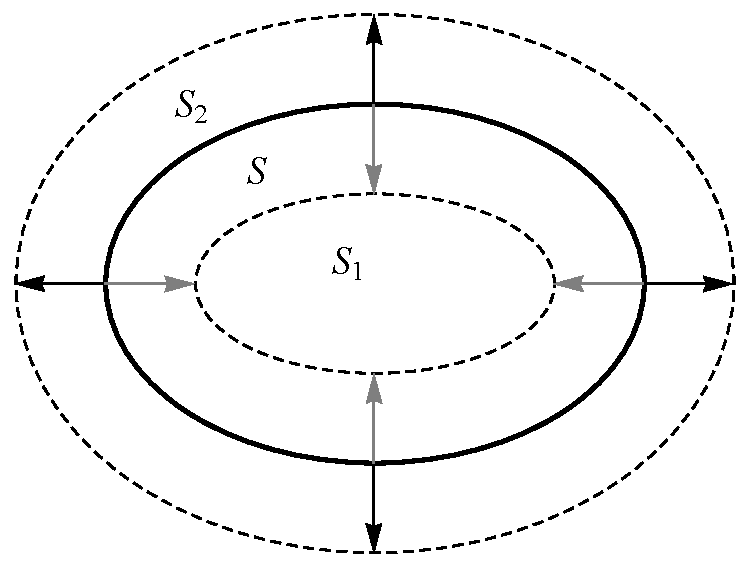
\includegraphics[scale=0.4]{inout.pdf}
\caption{From surface $S$, ingoing geodesics produce a smaller surface $S_1$ with area $A_1$ after a time $t=\epsilon$, while outgoing geodesics form a larger surface $S_2$ with area $A_2$. This is the behaviour of ingoing and outgoing expansions in a flat spacetime and the surfaces $S_1$ and $S_2$ are known as normal surfaces.}\label{figexp} 
\end{figure}

However, at points close to a singularity, these expansions can behave very differently. For example, inside the event horizon of a Schwarzschild black hole, with $r<2GM$, both sets of geodesics would form a surface of smaller area, after a given time has passed. The resulting surfaces are known as \emph{trapped surfaces}, the existence of which strongly suggests and, in some case, necessitates the formation of a singularity. In broad strokes, we may say that singularities are an inevitable consequence of trapped surfaces, in a geometrically-flat or open Universe, so long as positive energy density is maintained \cite{tHooft:2009bh}. However, this is not necessarily the case for a closed Universe, see \cite{Ellis:2003mb}.

There is another type of surface called an \emph{antitrapped surface}, which is formed when the expansion is rapid enough that both in- and outgoing tangent vectors form a surface of a larger area after a given time has passed. A {minimally antitrapped surface} (MAS) has vanishing outgoing expansion and any surface greater in radius to the MAS will necessarily be antitrapped. Furthermore, an apparent horizon is found on the inner boundary of the MAS, like so
\[
\label{mashorizon}
x_{mas}=H^{-1}
,\]
where $x_{mas}$ is the physical size of the minimally antitrapped surface. We will return to this relation to the the apparent horizon shortly, but conclude here with a summary of the surfaces we have introduced:
\begin{align}
\mbox{Normal Surface:}&\qquad \theta_{IN}<0\mbox{ and } \theta_{OUT}>0
\\ \mbox{Trapped Surface:}&\qquad \theta_{IN}<0\mbox{ and } \theta_{OUT}<0
\\ \mbox{Antitrapped Surface:}&\qquad \theta_{IN}>0\mbox{ and } \theta_{OUT}>0.
\end{align}
Further note that surfaces termed \emph{marginally trapped}, are those with negative expansions as opposed to negative definite, i.e. marginally trapped surfaces include those with vanishing expansion and are defined by simply replacing the $<$ sign with $\leq$, above. Similarly for \emph{marginally antitrapped} surfaces, $>$ is replaced with $\geq$. 
\subsubsection*{Cosmological Expansion}
In order to understand more clearly the nature of these surfaces, it is pertinent to derive the exact form of the ingoing and outgoing expansions in a cosmological setting. To this end, we invoke the  spatially flat, homogenous and isotropic Friedmann-Robertson-Walker (FRW) metric
\[
\label{FRWsphere}
ds^{2}=-dt^{2}+a^{2}(t)\left(dr^{2}+r^{2}d\Omega^{2}\right)
 . \]
Recall from \eqref{expshtw}, that we may write the expansion $\theta$ as follows
\[
\theta=\partial_{\mu}k^{\mu}+\Gamma_{\mu\sigma}^{\mu}k^{\sigma}.
\]
We also note that the two geodesic equations for the time and spatial coordinate read
\[
\frac{d^{2}t}{d\lambda^{2}}+a\dot{a}\delta_{ij}\frac{dx^{i}}{d\lambda}\frac{dx^{j}}{d\lambda}=0,\qquad
\frac{d^{2}x^{i}}{d\lambda^{2}}+\frac{\dot{a}}{a}\frac{dt}{d\lambda}\frac{dx^{i}}{d\lambda}=0
, \]
respectively, where $\lambda$ is an affine parameter.
Without loss of generality, we may consider paths along the $x$-direction only \footnote{where, at this time, we are considering the isotropic form of \eqref{FRWsphere} with $dr^{2}+r^{2}d\Omega^{2}=dx^2+dy^2+dz^2$}, with $x^{\mu}(\lambda)=\{t(\lambda),x(\lambda),0,0\}$. For $ds^{2}\rvert_{\mbox{{\tiny null}}}=0$, we then have
\[
dt^{2}=a^{2}(t)dx^{2},\qquad \implies \qquad \frac{dx}{d\lambda}=\frac{1}{a}\frac{dt}{d\lambda}.
 \]
Substituting this latter identity into the geodesic equation for the time coordinate gives
\[
\frac{d^{2}t}{d\lambda^{2}}+\frac{\dot{a}}{a}\left(\frac{dt}{d\lambda}\right)^{2}=0
 \]
One can easily verify that $d\lambda=\frac{a}{N}dt$ with constant $N$ is a solution of this equation. Setting $N$ to unity we find
\[
\left(\frac{dt}{d\lambda},\frac{dx^{i}}{d\lambda}\right)=\left(\frac{1}{a},\frac{1}{a^{2}}\right)
. \]
Due to the isotropic nature of the FRW metric \eqref{FRWsphere}, the spatial components are equal and can therefore be truncated into  the index $i=\{1,2,3\}$~\footnote{Greek indices indicate spatial and temporal components, i.e. $\mu,\nu,\lambda,\ldots=\{0,1,2,3\}$, whereas Latin letters indicate the spatial components $i,j,k,\ldots=\{1,2,3\}$}. We may now express $k^{\mu}$, the tangential vector field to the congruence of null geodesics, as follows
\[
\label{nullgeo}
k^{\mu}=\left(\frac{1}{a},\pm\frac{1}{a^{2}}\right)=(k^{0},k^{i}),
 \]
where the sign attached to $k^i$ is negative for ingoing rays and positive for outgoing rays. The final step is to compute the expansion, itself. To this end, we note that the expansion can be rewritten in the following form
\[
\theta\equiv\frac{1}{\sqrt{g}}\partial_\mu(\sqrt{g} k^\mu )
\]
For the FRW metric given in \eqref{FRWsphere}, we have $g=|\det(g_{\mu\nu})|=a^6 r^4 \sin^2\psi$, allowing us to write the ingoing and outgoing expansion for the given cosmological spacetime
\[
\label{nullgeoinout}
\theta_{IN}=\frac{2}{a(t)}\left(\frac{\dot{a}}{a}-\frac{1}{ra}\right),\qquad\theta_{OUT}=\frac{2}{a(t)}\left(\frac{\dot{a}}{a}+\frac{1}{ra}\right)
. \]
\cite{Vilenkin:2014yva},\cite{Vachaspati:1998dy}.
\subsubsection*{Cosmological Apparent Horizons and Conformal Diagram}
The first thing to note from these ingoing and outgoing expansions is that the term $x\equiv ra$ denotes the physical size of the surface described by the expansion in a geometrically-flat spacetime. This can be seen by the general formula for comoving distance of a general FRW metric, which is given by \cite{Berera:2000xz}
\[
x\equiv a\int dr (1-kr^2)^{-\frac{1}{2}}=ar,\mbox{ when } k=0.
\]
As the inner boundary of an antitrapped surface is the region where the surface becomes \emph{marginal}, by definition, this region will have vanishing expansion. Thus, we may justify the assertion \eqref{mashorizon} that the minimally antitrapped surface is bounded by an apparent horizon on its inner margin, upon reference to the ingoing expansion given in \eqref{nullgeoinout}. By setting \eqref{nullgeoinout} to zero, we find that for a comoving distance $r_{mas}$, we have
\[
x_{mas}=H_{FRW}^{-1}
,\] 
where $H_{FRW}$ is the cosmological apparent horizon of the FRW background \cite{Berera:2000xz}, \cite{Vachaspati:1998dy},\cite{tHooft:2009bh},\cite{d1992approaches}.

\subsubsection*{Accelerated Expansion of the Universe} Inflation theory suggests a period of rapid expansion soon after the  Big Bang is required for the formation of the large scale structures we see today. Whereas, expansion slows after this inflationary period, observational data has found that the Universe is still undergoing accelerated expansion at present \cite{Accel}. In terms of the FRW metric \eqref{FRWsphere}, accelerated expansion of the universe is defined by
\[
\label{acc}
\ddot{a}>0,\qquad\mbox{equivalently}\qquad {\dot H}+H^2>0
.\]
On comparing this with the curvature scalar in FRW, $R=6\left(\dot{H}+2H^2+\frac{k}{a^2}\right)$, we find that in a period of accelerated expansion, the curvature scalar $R$ is always positive, at least in a geometrically flat or open Universe. Fig. \ref{bigbang} illustrates  such inflation within a Big Bang cosmology. 

\begin{figure}[h]\cite{Vachaspati:1998dy},\cite{Berera:2000xz}
\centering
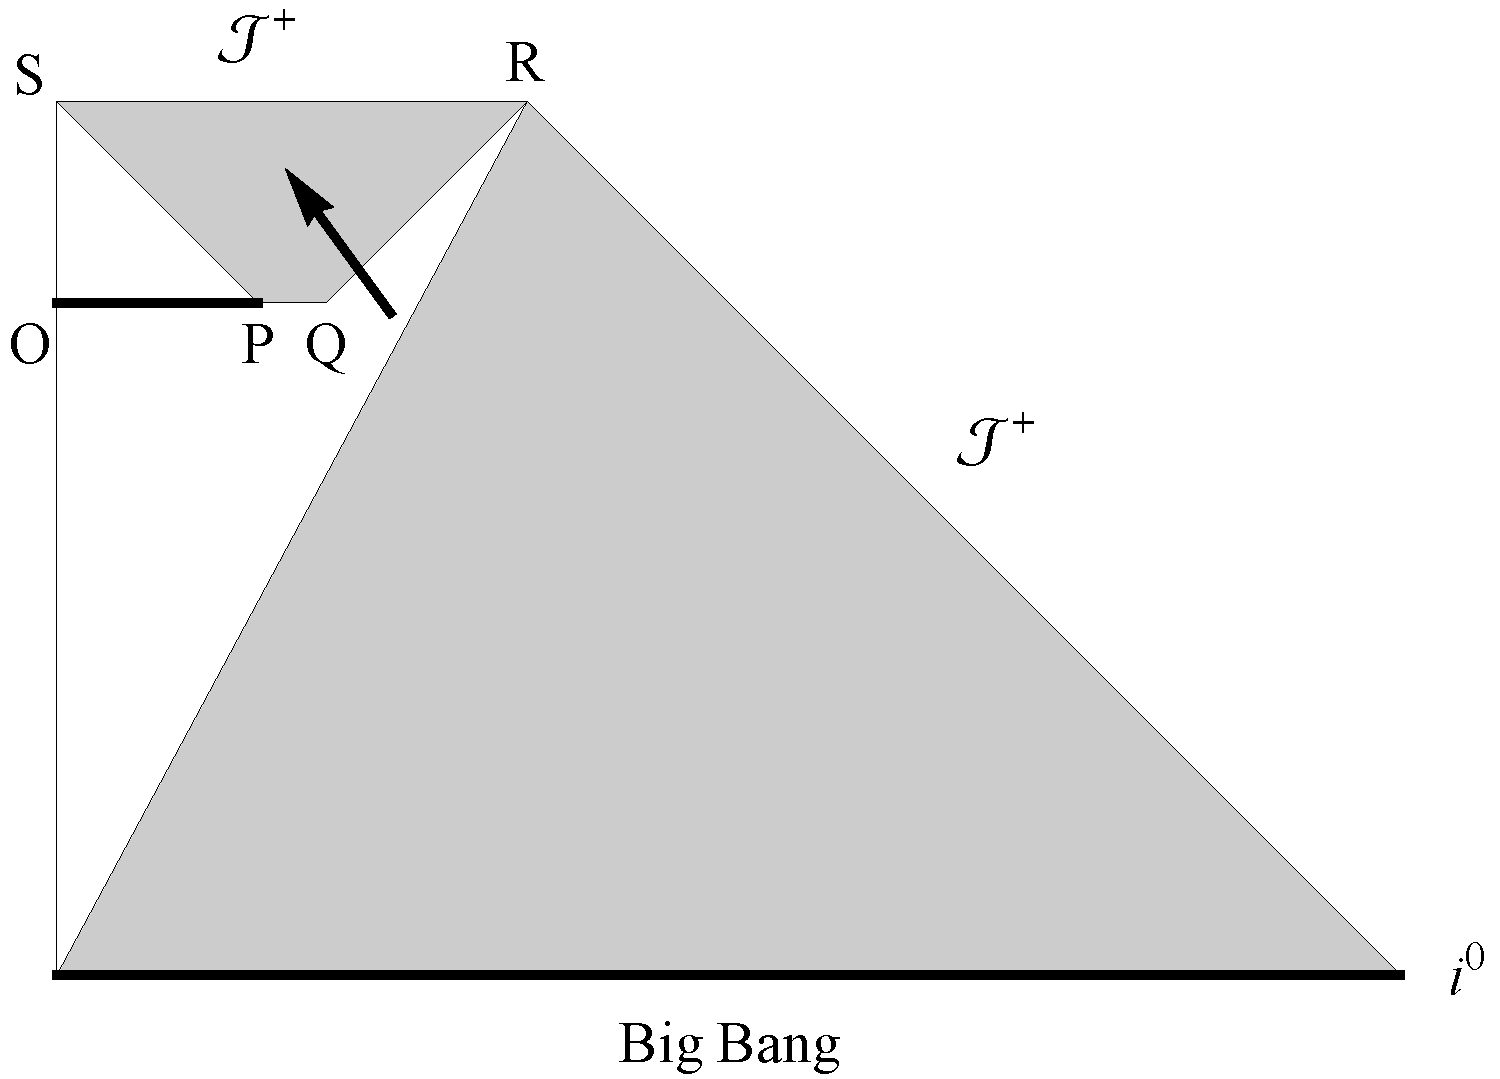
\includegraphics[scale=0.4]{bigbang.pdf}
\caption{A conformal diagram of a Big Bang cosmology with local inflation. Shaded regions are antitrapped and white regions are normal surfaces. A patch begins to inflate at cosmic time $t$ from $O$ to $Q$ with inflationary size $x_{\text {\it inf}}$, where the line $OP$ borders the apparent inflationary horizon. The arrow depicts an ingoing null ray entering an antitrapped region from a normal region, which is prohibited under the convergence condition \eqref{nullCC}. The inflationary patch $OQ$ may indeed be extended into the antitrapped region so that no such violation occurs.}\label{bigbang} 
\end{figure}


\subsubsection*{Null vs. Timelike Geodesic Congruences}
We stated earlier that null geodesic congruences more readily converge than their timelike counterparts and therefore, an analysis of null rays is more illuminating in terms of defocusing and past-completeness. In this section, we will show that if a geometrically-flat spacetime is singularity-free in the context of null rays, its timelike counterpart will necessarily be singularity-free. For our purposes here, we begin with the isotropic form of the FRW metric
 \[
 ds^2=-dt^2+a^2(t)(dx^2+dy^2+dz^2)
, \]
while following closely to \cite{Albareti:2014dxa}. We then compute the null and timelike convergence conditions, which are
\[
a\ddot{a}\leq\dot{a}^{2},\qquad a\ddot{a}\leq\frac{\dot{a}^{2}}{1+\frac{3a^{2}}{2\gamma_{0}^{2}v_{0}^{2}u_{0}^{2}}}
 \]
 respectively. Here, the timelike vector field is taken to be of the form $\xi^\mu=\gamma(1,\nu^i)$, where $\gamma\equiv \frac{1}{\sqrt{1-a^2 v^2}}$; and the subscript $_0$ refers to the quantities being evaluated at $t=t_0$. Further details can be found in \cite{Albareti:2014dxa}. For the present discussion, the precise details of these quantities are not strictly relevant. We simply note that the respective convergence conditions take the form
 \[
 a\ddot{a}\leq\dot{a}^{2},\qquad a\ddot{a}\leq\frac{\dot{a}^2}{1+A^2}
\]
with $A^{2}=\frac{3a^{2}}{2\gamma_{0}^{2}v_{0}^{2}u_{0}^{2}}$, being a positive parameter. The limiting case of the null convergence condition can be found by framing the left inequality as an identity and solving the differential equation. We find this to take the form 
\[
a(t)=c_0 e^{c_1 t},
\]
for some integration constants $c_0,c_1$. Pleasingly, this conforms to the scale factor in de Sitter space,
\[
a(t)=a_0 e^{\bar{H} t}
,\]
where ${\bar H}$ is the Hubble constant \cite{Albareti:2014dxa}. Comparing this with the timelike case and we find that of the two convergence conditions, the null CC is less restrictive. In other words, timelike geodesics are more easily made past-complete by this condition and so, in a study of singularity-free cosmologies, it makes sense to study null rays over their timelike counterparts. To summarise, in a geometrically-flat cosmology, if a spacetime is non-singular for null rays, it will also be devoid of singularities for timelike geodesics.
%\\\\\emph{Deceleration parameter}\\
%These may then be expressed using the deceleration parameter $q\equiv-\frac{1}{H^{2}}\frac{\ddot{a}}{a}$, so that
%\[
%q_{null}\geq-1,\qquad q_{timelike}\geq-\frac{1}{1+A^{2}}
%.\]
%For very large $A$, these inequalities becomes
%\[
%q_{null}\geq-1,\qquad q_{timelike}\geq 0
%,\]
%which is exactly the limits of the deceleration parameter given by requiring the null energy condition and the strong energy condition, respectively, which, in turn, account for congruences of null and timelike geodesics, respectively. It should now be clear that the null CC is more easily satisfied, i.e. geodesics more readily converge in the null sense.
%\subsection{Trapped Surfaces in a Closed Universe}
%Ellis - trapped surfaces do not always 
\section{Defocusing Conditions for Infinite Derivative Gravity around Minkowski Space}
\label{sec:defocusmink}
In this section, we extend our study of geodesic congruences away from general relativity  into the novel approach of infinite derivative gravity (IDG), the groundwork of which was laid in Chapter \ref{chap:2}, where the non-linear and linearised equations of motion were derived and in Chapter \ref{chap:GF}, where the theory was rendered free of ghosts and tachyons. It is now time to return to the central question of this thesis, first raised in the Introduction, by asking the question:
\begin{quote}
\emph{Can null rays defocus in an infinite derivative theory of gravity, without introducing ghosts, tachyons or exotic matter?}
\end{quote}
In essence, we wish to show how infinite derivative extensions of gravity, in contrast to GR and finite  models, have the potential to describe a stable and singularity-free theory of gravity. 
\\\\
Recall that in Section \ref{sec:linkmink}, we derived the linearised field equations for the infinite derivative action of gravity:
\[
\label{actionRE}
S=\frac{1}{2}\int d^4x \sqrt{-g}\biggl(M_P^2 R+R{\cal F}_1(\Box)R+R^{\mu\nu}{\cal F}_2(\Box)R_{\mu\nu}+C^{\mu\nu\lambda\sigma}{\cal F}_3(\Box)C_{\mu\nu\lambda\sigma}\biggr)
,\]
where, within the form factors ${\cal F}_i(\Box)=\sum^\infty_{n=0}(\Box/M^2)^n$, each D'Alembertian operator is modulated by the scale of non-locality $M$. The resulting field equations are given by
\[
\label{eomminkRE}
\kappa T_{\mu\nu}=a(\Box)R_{\mu\nu}-\frac{1}{2}\eta_{\mu\nu} c(\Box)R-\frac{f(\Box)}{2}\partial_\mu \partial_\nu R
,\]
where the infinite derivative functions $a(\Box),c(\Box),f(\Box)$ are made up of the form factors ${\cal F}_i(\Box)$, defined in \eqref{abc}, and conform to the constraint
\[
f(\Box)\Box=a(\Box)-c(\Box)
.\]
Furthermore, through our lengthy discussion on the Raychaudhuri equation in General Relativity in Section \ref{sec:RE}, we learned of its powerful role in conveying the focusing behaviour of geodesic congruences, where the sole contribution of gravity stems from the $R_{\mu\nu}k^\mu k^\nu$ term, with $k^\mu$ representing a null tangent vector or ray. We may then find the contribution of gravity to the RE for the infinite derivative theory of gravity, described by the action \eqref{actionRE}, by contracting the linearised field equations \eqref{eomminkRE} with the tangent vectors $k^\mu$. Thus, we obtain the \emph{IDG convergence condition}
\[
\label{convergeIDG}
R_{\mu\nu} k^\mu k^\nu=a^{-1}(\Box)\biggl(\kappa T_{\mu\nu}k^\mu k^\nu +\frac{1}{2}k^\mu k^\nu f(\Box)\partial_\mu \partial_\nu R\biggr)\geq 0
.\]
If a theory satisfies this condition, the associated null rays cannot start to diverge until they reach the origin. In other words, these null rays converge towards a singularity in a finite time, as is the behaviour in GR. However, in contrast to GR, where $R_{\mu\nu}k^\mu k^\nu$ 
%$R_{\mu\nu}k^\mu k^\nu = \kappa T_{\mu\nu}k^\mu k^\nu\geq 0$
 must remain positive so as  not to violate the null energy condition \eqref{NEC}, we have modified the stress-energy tensor in such a way that it may indeed be possible to reverse the sign of $R_{\mu\nu}k^\mu k^\nu$ whilst retaining the NEC. We call the inequality $R_{\mu\nu}k^\mu k^\nu<0$ the \emph{defocusing condition}, as it is the condition whereby null rays may defocus, suggestive of a singularity-free theory of gravity.

\subsubsection*{Homogenous Solution.}
The linearised field equations \eqref{eomminkRE} describe the curvature of a spacetime that has been perturbed away from Minkowski space. We begin our analysis by discussing perturbations that are entirely homogenous, with all curvature dependent only on the cosmic time $t$. One could think of the time-dependent, perturbed metric $h_{ij}$ which makes up the curvature, as being closely related to the cosmological scale factor of FRW, which is useful in this context, as we are considering cosmological singularities. In the homogenous case, the D'Alembertian simply becomes $\Box=-\partial_t^2$, so that the defocusing condition $R_{\mu\nu}k^\mu k^\nu<0$ reads \cite{Conroy:2016sac}
\[
\label{divergemink1}
R_{\mu\nu} k^\mu k^\nu=a^{-1}(\Box)\biggl(\kappa T_{\mu\nu}k^\mu k^\nu -\frac{1}{2}k^\mu k^\nu f(\Box)\Box R\biggr)< 0
,\]
where in order to preserve the NEC, we have $T_{\mu\nu}k^\mu k^\nu\geq 0$. We may then say that the minimum requirement for such a theory to display the desired defocusing behaviour is given by
\[
\frac{f(\Box)\Box}{a(\Box)} R= \frac{a(\Box)-c(\Box)}{a(\Box)} R>0
\label{divergemink2}
,\]
with $T_{\mu\nu}k^\mu k^\nu$ set to zero.
%\textcolor{Blue}{In essence here, we have set $T_{\mu\nu}k^\mu k^\nu=0$ to find the minimum defocusing condition, which is illustrative. One can repeat this for general $T_{\mu\nu}k^\mu k^\nu$ with slightly messier results. Question is though, as $T_{\mu\nu}k^\mu k^\nu=\rho+p$, if $T_{\mu\nu}k^\mu k^\nu=0$ then $\rho=-p$ and by the equation of state $p=w\rho$, $w$ in this case would be $-1$, which is the equation of state for the cosmological constant. Does this mean that this perturbed metric is essential dS?}
Immediately, we are confronted with some important observations, which we outline below.
\subsubsection*{Observations}
\begin{enumerate}
\item[$a=c:$] If we recall the form of the modified graviton propagator from Section \ref{sec:prop}
\[
\label{propmink}
\Pi(-k^{2})=\frac{\mathcal{P}^{2}}{k^{2}a(-k^{2})}+\frac{\mathcal{P}_{s}^{0}}{k^{2}\left(a(-k^{2})-3c(-k^{2})\right)},
\]  
we find that the condition $a(\Box)=c(\Box)$ necessitates that no additional pole, other than the massless graviton, is introduced. In this case, the modified propagator is simply the physical graviton propagator modulated by an overall factor of $\sim 1/a(\Box)$, where the function $a(\Box)$ is an exponent of an entire function, containing no roots:
\[
\label{defocus0}
\Pi(-k^{2})=\frac{1}{a(-k^{2})}\biggl(\frac{\mathcal{P}^{2}}{k^2}-\frac{\mathcal{P}_{s}^{0}}{2k^2}\biggr)
.\] 
The curvature $R$ is positive as a result of accelerated expansion of the Universe, Section \ref{sec:RE}, so that from \eqref{divergemink1}, we see that the defocusing condition can only be achieved if $a(\Box)$ is negative when acting on the curvature. As should be apparent from the above form of the propagator, such a negative function would reverse the sign of the spin-2 component, leading to a negative residue and subsequently a ghost. This ghost is known as the \emph{Weyl ghost} and was discussed in Section \ref{sec:patho}. As a result, we conclude that an \emph{additional scalar degree of freedom is required} in order for null rays to display the desired defocusing behaviour.  

\item[$a\neq c:$] Having established the  need for a departure from the pure massless mode of the graviton propagator
in \eqref{propmink}, we move into the more general case of $a(\Box)\neq c(\Box)$. This condition tells us that in order for the null rays to defocus - a minimum requirement of a singularity-free theory of gravity - one requires an additional root in the spin-0 component of the graviton propagator. As such, one additional scalar degree of freedom must propagate in the spacetime besides the massless graviton, if we wish to satisfy the defocusing condition.  As $a(\Box)$ does not introduce a new pole, the spin-2 component of the graviton
propagator remains massless. 
\end{enumerate}
~\\We have already demonstrated a significant departure from general relativity, in that IDG corrections have allowed for the possibility of singularity avoidance, via the defocusing condition \eqref{defocus0}, without violating the null energy condition. 

Having established the need for an additional pole in the propagator, we must now take steps to avoid the introduction of ghosts or tachyons. In  Section \ref{sec:GF}, we derived the ghost-free condition around a Minkowski background. This condition took the form
\[
\label{GFrepeat}
c(\Box)=\frac{a(\Box)}{3}\left[1+2(1-\alpha M_P^{-2}\Box){\tilde a}(\Box)\right]
, \]
where the constant $\alpha=6f_{1_{0}}+2f_{2_{0}}-M_{P}^{2}/M^{2}$ and ${\tilde a}(\Box)$ is an exponent of an entire function, containing no roots. Substitution into \eqref{propmink} reveals the ghost-free modified propagator for an asymptotically-flat spacetime:
\[
\label{MinkPropdec}
\Pi(-k^{2})=\frac{1}{a(-k^{2})}\biggl[\frac{{\cal P}^{2}}{k^{2}}-\frac{1}{2\tilde{a}(-k^{2})}\biggl(\frac{{\cal P}_{2}^{0}}{k^{2}}-\frac{{\cal P}_{s}^{0}}{k^{2}+m^{2}}\biggr)\biggr]
, \]
where we have defined
\[
\label{Staro-mass}
m^2=M_P^2/\alpha
.\]
$m^2$ must be positive to ensure that the mass is non-tachyonic and $\alpha$ positive definite in order to retain the essential new pole, i.e. the constant $\alpha=6f_{1_{0}}+2f_{2_{0}}-M_{P}^{2}/M^{2}$ satisfies $\alpha>0$. Armed with this, we are now in a position to describe the defocusing condition which precludes the existence of ghosts. Substitution of \eqref{GFrepeat} into \eqref{divergemink2} leads to the central result
\[
\label{defocusmink}
(1-\Box/m^2){\tilde a}(\Box)R<R
.\]
\subsection{Comparison with Starobinsky Model}
Taking the limit $M \rightarrow \infty$, with  ${\cal F}_2={\cal F}_3=0$, reduces the action \eqref{action} to that of Starobinsky's model of 
inflation~\cite{Starobinsky:1979ty}. Indeed, a curious question to ask is, could Starobinsky's action avoid the cosmological singularity? At the limit $M\rightarrow \infty$,  the propagator \eqref{propmink} can be expressed as
\[
\label{propR2}
\Pi_{R^{2}}=\Pi_{GR}+\frac{1}{2}\frac{\mathcal{P}_{s}^{0}}{k^{2}+m^{2}} ,
\]
where $m$ is given by (\ref{Staro-mass}), with $\alpha=6f_{1_0}\geq 0$, and $m^2>0$, to avoid tachyonic mass.
 However, the fundamental difference can be seen by comparing the propagator for $R^2$-gravity with the IDG propagator, \eqref{MinkPropdec}.  In the local limit, $a(\Box)={\widetilde a}(\Box)\rightarrow 1$. Furthermore, as we are making comparisons with the propagator in momentum space, the D'Alembertian takes the form $\Box\rightarrow -k^2$. In this case, the defocusing inequality \eqref{divergemink1} can only be satisfied for 
\[
m^{-2} R<0
.\]
In this scenario, to avoid focusing we require $m^2< 0$, rendering the theory tachyonic. Alternatively, negative curvature would contradict the requirement of accelerated expansion of the Universe, see \eqref{acc}, which is vital to realise primordial inflation, Section \ref{sec:patho}. As such, the Starobinsky model cannot pair inflation with resolving the Big Bang Singularity.
\section{Bouncing Solution}
\label{sec:Bouncing}
\begin{figure}[h]\cite{Conroy:2014dja}
\centering
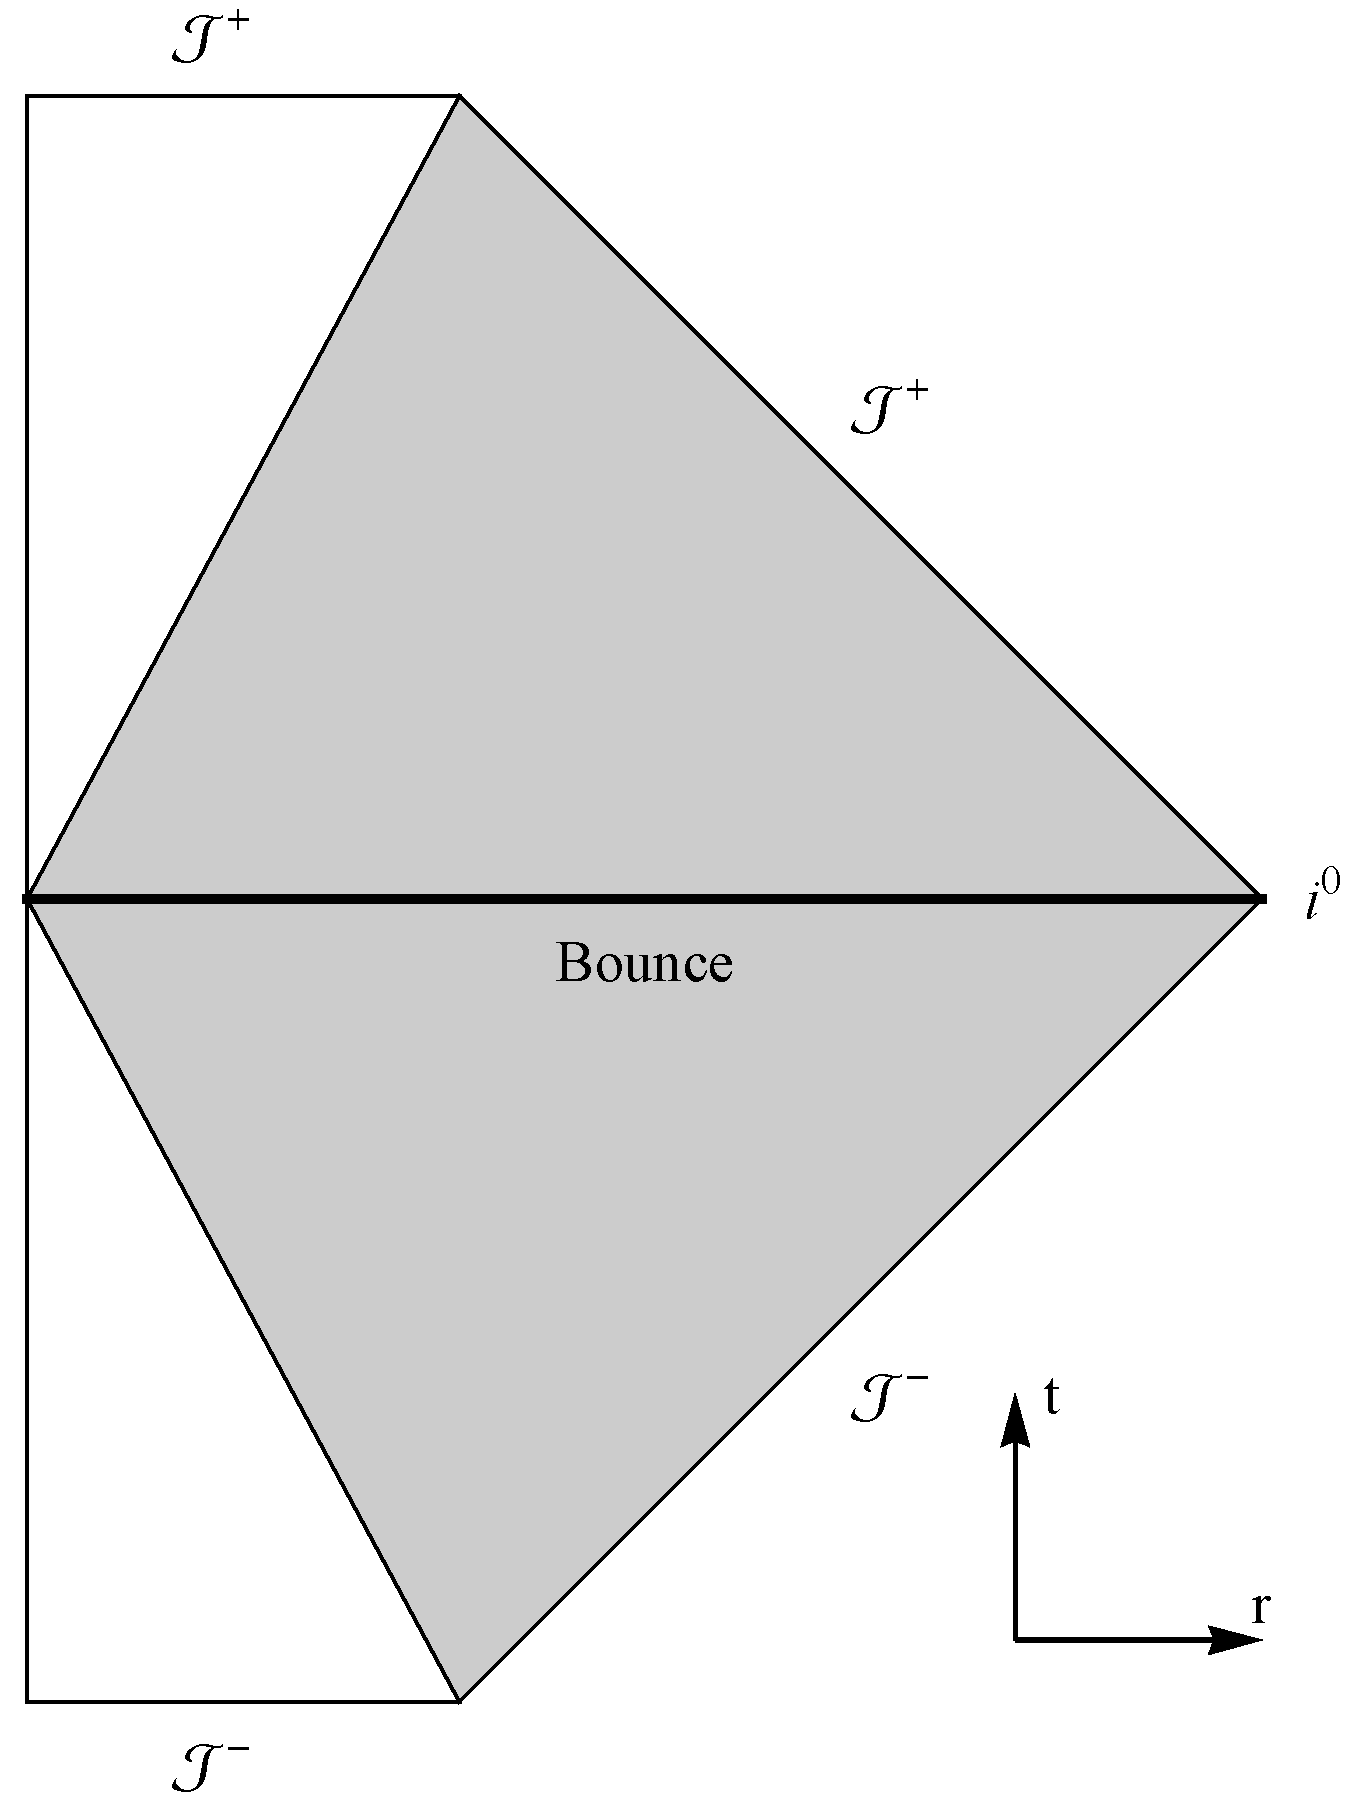
\includegraphics[scale=0.3]{bounce2.pdf}
\caption{A conformal diagram depicting a bouncing cosmology, seen as an extension of Fig. \eqref{bigbang} into past infinity. Shaded regions are antitrapped surfaces, bordered by a cosmological apparent horizon on their inner margins and white regions are normal surfaces.} \label{figbounce} 
\end{figure}
Up to this point, we have not spoken about what replaces the Big Bang singularity in a non-singular spacetime. 
This is because, as opposed to \cite{Conroy:2014dja},\cite{Koshelev:2012qn},\cite{Koshelev:2013lfm},\cite{Biswas:2011ar},\cite{Abramo:2009qk}, we have made no assumptions on the nature of the cosmological scale factor, which is closely related to the perturbed metric tensor $h_{\mu\nu}$. The term scale factor is most often associated with the function $a(t)$ in an FRW metric \eqref{FRWsphere}. However, in an homogeneous and isotropic spacetime such as the one we are considering around Minkowski space, we note that we are very closely aligned to the FRW metric, making cosmological predictions relevant. In this way, the metric can be considered to be of the form
\[
g_{\mu\nu}=\eta_{\mu\nu}+h_{\mu\nu}=\{-1,a^2(t),a^2(t),a^2(t)\}
.\]
Bouncing cosmologies replace the initial big bang singularity with that of a bounce, so that incoming geodesic congruences can be made past complete - stretching to past infinity, leading to an extension of the conformal diagram Fig. \ref{bigbang}, which is illustrated in Fig. \ref{figbounce}. Although, we do not suppose a priori that the initial singularity is replaced by a bounce, we would indeed expect cosmologies with a bouncing scale factor to satisfy the defocusing condition \eqref{defocusmink}. 

\noindent We illustrate this by way of example.
\subsection{Integral Form}
It may now be illuminating to test our defocusing condition \eqref{defocusmink}. We proceed, as in the Starobinsky case, by taking our analysis into momentum space and testing against a well-known \emph{bouncing solution}, that is, a cosmology defined by a bouncing scale factor, which is necessarily an even function. However, due to the infinite derivative nature of the function ${\tilde a}(\Box)$, this comes with an added degree of complexity. One possibility in analysing the defocusing condition \eqref{defocusmink}  lies in recasting the defocusing condition into its integral form \cite{reed1975methods}.
\newpage
\noindent\emph{Integral Form}\\
As discussed in Chapter \ref{chap:GF}, we must choose ${\tilde a}(\Box)$ to be an exponent of an entire function, the simplest case being~\footnote{We note briefly the importance of the sign in the exponent of ${\tilde a}(\Box)$. In Appendix \ref{chap:NewtPot},\cite{Edholm:2016hbt},\cite{Biswas:2011ar}, it is shown that for the correct Newtonian potential to be observed, the non-local function $a(\Box)$ must be of the form $a(\Box)=e^{-\gamma(\Box)}$, where $\gamma(\Box)$ is an entire function. As ${\tilde a}(\Box)$ is defined as ${\tilde a}(\Box)\propto 1/a(\Box)$, and both are defined as exponents of entire functions, it is reasonable to expect a difference of a minus sign in the exponent.} 
\[
{\tilde a}(\Box)=e^{\Box/M^2}
,\]
where, again, $M$ is the scale of non-locality. Thus, we wish to compute $e^{\Box/M^2}R(t)$, where $R(t)$ is the curvature scalar, solely dependent on $t$. To this end, we reformulate this expression into its integral form by first defining the Fourier transform and its inverse like so
\[
\hat{R}(k)\equiv\frac{1}{\sqrt{2\pi}}\int_{-\infty}^{\infty}e^{ikt}\tilde{R}(t)dt,\qquad R(t)\equiv\frac{1}{\sqrt{2\pi}}\int_{-\infty}^{\infty}e^{-ikt}\hat{R}(k)dk
.\]
We may then write
\[
{\tilde a}(\Box)R(t)	=	\frac{1}{\sqrt{2\pi}}\int_{-\infty}^{\infty}\exp(-k^{2}/M^{2})\exp(-ikt)\hat{R}(k)\;dk
.\]
By using the properties of the Fourier transform and defining $x\equiv k/M$, we may express this as follows
%\[
%e^{\Box/M^2}R(t)=\frac{1}{\sqrt{2\pi}}\int_{-\infty}^{\infty}\exp(-k^{2}/M^{2}+ik(\tau-t))\left(\frac{1}{\sqrt{2\pi}}\int\hat{R}(\tau)d\tau\right)\;dk
%.\]
%By defining $x\equiv k/M$, we can express this as
\[
{\tilde{a}}(\Box)R(t)=\frac{M}{2\pi}\int\int_{-\infty}^{\infty}\exp\left[-x^{2}+ix\left(M(\tau-t)\right)\right]\hat{R}(\tau)\;dx\;d\tau
.\]
Now, in order to compute in terms of the Gaussian integral
$
\int_{-\infty}^{\infty}\exp\left(-a(x+b)^{2}\right)dx=\sqrt{\frac{\pi}{a}}
$,
we rewrite ${\tilde a}(\Box)R(t)$ into the following form
\begin{align}{\tilde{a}}(\Box)R(t)=\frac{M}{2\pi} & \int\int_{-\infty}^{\infty}\exp\left[-\left(x-\frac{i}{2}\left(M(\tau-t)\right)\right)^{2}-\frac{1}{4}\left(M(\tau-t)\right)^{2}\right]\hat{R}(\tau)\;dx\;d\tau.\end{align}
We then compute the Gaussian integral to find
\[
{\tilde a}(\Box)R(t)=\frac{M}{2\sqrt{\pi}}\int_{-\infty}^{\infty}e^{-\frac{1}{4}M^2(\tau-t)^{2}}\hat{R}(\tau)d\tau
.\]
Similarly,
\[
-\Box/m^{2}\tilde{a}(\Box)R(t)=\frac{M^{3}}{8\sqrt{\pi}m^{2}}\int_{-\infty}^{\infty}e^{-\frac{1}{4}M^{2}(t-\tau)^{2}}\left(2-M^{2}(t-\tau)^{2}\right)\hat{R}(\tau)d\tau
.\]
The defocusing condition \eqref{defocusmink} can then be written as
\[
\label{defocusint}
\frac{M}{2\sqrt{\pi}}\biggl[\int_{-\infty}^{\infty} e^{-\frac{1}{4}M^2(\tau-t)^{2}}\biggl(1+\frac{M^{2}}{2m^{2}}-\frac{M^{4}}{4m^{2}}(t-\tau)^{2}\biggr)\hat{R}(\tau)d\tau<R(t)
\]
\\\subsubsection*{Example: $a(t)=\cosh\frac{\sigma}{2} t$}
We now turn to a particular example of a bouncing solution. In this case, we assume a scale factor of $a(t)=\cosh\frac{\sigma}{2} t$, where $\sigma$ is a  parameter of mass dimension. Solutions of this type have been studied extensively in \cite{Koshelev:2012qn},\cite{Koshelev:2013lfm},\cite{Biswas:2005qr} and found to be a solution of the field equations \eqref{eomfull}, via an Ansatz-based approach. In terms of the perturbed, t-dependent metric $h_{\mu\nu}$, this scale factor can be written as
\[
h_{\mu\nu}=\biggl\{0,\;\cosh^2(\frac{\sigma t}{2})-1,\;\cosh^2(\frac{\sigma t}{2})-1,\;\cosh^2(\frac{\sigma t}{2})-1\biggr\}.
\]
%line element
%\[
%ds^{2}=-dt^{2}+\left(1+\cosh^{2}(\frac{\sigma}{2}t)\right)dr^{2}
%\]
Then, from the definition of curvature around Minkowski, \eqref{MinkR}, we find the curvature to be
\[
R(t)=\frac{3}{2}\sigma^2 \cosh\sigma t
.\]
We then substitute this form of the curvature into the defocusing condition \eqref{defocusint} and compute the integral to find that, for any cosmic time $t$, defocusing may be realised according to
\[
\frac{\sigma^{2}}{m^{2}}>(1-e^{-\frac{\sigma^{2}}{M^{2}}}).
\]
%\[
%(m-\sigma)(m+\sigma)\left(\sinh\left(\frac{\sigma^{2}}{M^{2}}\right)+\cosh\left(\frac{\sigma^{2}}{M^{2}}\right)\right)<m^{2}
%.\]
%As $X^2\equiv\sinh\left(\frac{\sigma^{2}}{M^{2}}\right)+\cosh\left(\frac{\sigma^{2}}{M^{2}}\right)$ is always positive, we may rewrite this as follows,
%\[
%1-X^{-2}<\frac{\sigma^{2}}{m^{2}}
%.\]
This is satisfied for all real $\sigma$ such that $\sigma\neq0$,
%$\frac{\sigma^{2}}{M^{2}}\in$ Reals, such that $\frac{\sigma^{2}}{M^{2}}\neq0$, 
so that we have confirmed that a known bouncing scale factor does indeed display the desired ghost-free defocusing behaviour, according to the constraint \eqref{defocusmink}.
%\\\\\emph{Example: $R(t)=1+r_2 t^2$}\\
%By substituting $R(t)=1+r_2 t^2$ into the integral form of the defocusing condition \eqref{defocusint} and solving, we arrive at the constraint
%\[
%\frac{r_2}{M^2}< \frac{r_2}{m^2}
%.\]
%One can easily check that this inequality is satisfied for all $r_2\neq  0$ and $m^2\neq M^2$ according to 
%\[
%r_2 \gtrless 0,\qquad m^2 \lessgtr M^2
%.\]
%Thus, we have confirmed another known bouncing solution to satisfy the defocusing condition \eqref{defocusmink}.
%%In momentum space, where $\Box=-k^2$, the defocusing condition becomes
%%\[
%%\tilde{a}(-k^{2})R<\frac{m^{2}}{m^{2}+k^{2}}R
%%.\]
%%We then choose ${\tilde a}(\Box)$ to be an exponent of an entire function, as discussed in Chapter \ref{chap:GF}, the simplest case being ${\tilde a}(\Box)=e^{\Box/M^2}$~\footnote{We note briefly the importance of the sign in the exponent of ${\tilde a}(\Box)$. In Appendix \ref{chap:NewtPot},\cite{Edholm:2016hbt},\cite{Biswas:2011ar}, it is shown that for the correct Newtonian potential to be observed the non-local function $a(\Box)$ must be of the form $a(\Box)=e^{-\gamma(\Box)}$, where $\gamma(\Box)$ is an entire function. As ${\tilde a}(\Box)$ is defined as ${\tilde a}(\Box)\propto 1/a(\Box)$, and both are defined as exponents of entire functions, it is reasonable to expect a difference of a minus sign in the exponent. }. Thus, we have
%%\[
%%\tilde{a}(-k^{2})=e^{-k^2/M^2}
%%,\]
%%resulting in the inequality,
%%\[
%%e^{-k^{2}/M^{2}}R<\frac{m^{2}}{m^{2}+k^{2}}R.
%%\]
%%As we are considering only first order poles in the propagator, it is sufficient, for this illustrative example, to consider only up to linear order in $k$, such that
%%\[
%%1-\frac{k^2}{M^2}<1-\frac{k^2}{m^2}
%%.\]
%%We then find that in this particular case, the desired ghost-free, defocusing behaviour can only be achieved when
%%\[
%%m^2/M^2>1
%%,\]
%%where $m$ is the spin-0 particle introduced into the propagator and $M$ is the scale of non-locality, or the scale of correction of the IDG theory, itself. The limit $M\rightarrow\infty$ removes all non-locality from the system. It is clear that for non-tachyonic mass $m^2>0$, this inequality is not satisfied at this limit, replicating the behaviour in the Starobinsky limit. This is suggestive of the integral role that non-locality plays in formulating a non-singular cosmology.
%\paragraph{Inhomogenous Solutions}
%We briefly extend our results to inhomogenous spacetimes. We may expand the general defocusing condition \eqref{convergeIDG}, to include solutions, with spatial as well as temporal dependencies. Without loss of generality, we consider the perturbations along the $x$-direction, where $r=\sqrt{x^2+y^2+z^2}$.
%As before, we require $T_{\mu\nu}k^\mu k^\nu \geq 0$ so as not to violate the NEC. We then read off the minimum requirement for the associated null rays to defocus
%\[
%\frac{f(\bar\Box)}{a(\bar\Box)}\left(\partial_{t}^{2}+\partial_r^2\right)R^{(L)}<0
%,\]
%where $\partial_r^2=\partial_i\partial^i$ is the Laplace operator.
%
\section{A simpler action of gravity.}
\label{sec:simpler}
From the defocusing condition \eqref{divergemink1}, we can deduce the simplest infinite derivative action that can describe a singularity-free theory of gravity. The central components for defocusing are the functions $a(\Box)$ and $c(\Box)$, which, in order to achieve freedom from ghosts, are exponents of entire functions with zero roots and one root, respectively. These functions are in turn made up of the infinite derivative form factors ${\cal F}_i(\Box)$ with $i=\{1,2,3\}$, which make up the gravitational action \eqref{action}, as given by \eqref{abc}. Consequently,  upon inspection of \eqref{abc}, it appears that we may be able to `switch off' one or two of the form factors without changing the  nature of the  functions $a(\Box)$ or $c(\Box)$. 
\\\\ \emph{Non-linear Regime}\\
For example, by setting ${\cal F}_2=0$, whilst retaining the infinite derivative form factors ${\cal F}_1$ and ${\cal F}_3$ and noting that
in a conformally-flat background, such as FRW, (A)dS or Minkowski, the Weyl tensor vanishes on the background, the action \eqref{action} reduces to the following
\[
\label{actionsimp}
S_{NL}=\frac{1}{2}\int d^{4}x\sqrt{-g}\bigl[M_{P}^{2}R+ R{\cal F}_{1}(\Box)R\bigr]\,.
\]
This reduced action would clearly prove useful in a non-linear cosmological analysis, where the contribution of the Weyl tensor would be precisely zero, even with a non-zero form factor ${\cal F}_3$, but it may also prove to be of interest in the linearised regime.
\\\\\emph{Linearised Regime}\\
On inspection of the infinite derivative functions \eqref{abc} which make up the field equations in the linearised regime, it should be clear that it is possible to `switch off' any one of the form factors ${\cal F}_i$, whilst still retaining the infinite derivative nature of the functions $a,c,f$ and thus, not adversely affecting the theory. We may extend this further to switching off two of the form factors ${\cal F}_i$. Straightforward examples, include: setting ${\cal F}_1={\cal F}_3=0$ with
\ba
&a(\Box)=1+M_{P}^{-2}{\cal F}_{2}(\Box)\square\nn\\&
a(\Box)-3c(\Box)=-2+4M_{P}^{-2}{\cal F}_{2}(\Box)\square
  \ea
and ${\cal F}_1={\cal F}_2=0$:
\ba
&a(\Box)=1+2M_{P}^{-2}{\cal F}_{3}(\Box)\Box\nn\\&
a(\Box)-3c(\Box)=-2+12M_{P}^{-2}{\cal F}_{1}(\Box)\square,
  \ea
 which retain the infinite derivative modification of both the scalar and tensorial sectors of the propagator. Slightly less clear, however, is the proposition of setting ${\cal F}_2={\cal F}_3=0$. This results in a correction of the scalar sector of the propagator, while leaving the spin-2 sector of the propagator unmodified. In this instance the relevant sectors of the propagator can be obtained from \eqref{abc} and are given by
\ba
\nn
&a(\Box)=1
\\& a(\Box)-3c(\Box)=-2+12M_{P}^{-2}{\cal F}_{1}(\Box)\square,
 \ea
One can easily check, from \eqref{defocusmink}, that this is indeed sufficient to realise the desired ghost-free defocusing behaviour. It appears then, that the modification of the spin-2 component of the propagator - which is rootless and positive so as to avoid the Weyl ghost - does not play a leading role in singularity avoidance.    Furthermore, the simplicity of this case allows us to more easily convey defocusing conditions in more complicated scenarios, such as around de Sitter space, which is our next focus.
 
 \section{Defocusing Conditions around de Sitter Space}
 \label{sec:defocusdS}
Here, we extend our discussion to include ghost-free, defocusing conditions around the de Sitter spacetime, with the reduced action
\[
\label{actionred}
S=\frac{1}{2}\int d^4x\sqrt{-g}\biggl(M_P^2 R-2\Lambda+R {\cal F}(\Box)R\biggr)
.\]
As we have seen from the previous section on a \emph{simpler action of gravity}, this is adequate for our aims of describing a ghost- and singularity-free theory.
This reduced form is equivalent to setting ${\cal F}_2={\cal F}_3=0$ in the general action \eqref{action} and dropping the remaining subscript from the function ${\cal F}_1\equiv {\cal F}$, for convenience. 

From here, we can deduce the expected behaviour of the propagator around de Sitter space by inspecting the modified propagator around Minkowski \eqref{propmink}. Upon reference to \eqref{abc}, we find that, by imposing ${\cal F}_2={\cal F}_3=0$, the spin-2 or tensorial sector of the propagator is no longer modified and all subsequent corrections take place in the scalar sector. This is as expected due to the purely scalar modification of the Einstein-Hilbert action taking place in \eqref{actionred}. An exposition of the ghost-free conditions for the full action \eqref{action} has recently been discussed in \cite{Biswas:2016egy}, where the perturbed metric $h_{\mu\nu}$ is decomposed into its 10 individual degrees of freedom via
\[
h_{\mu\nu}=h_{\mu\nu}^\perp+\nabla_\mu A_\nu^\perp+\nabla_\nu A_\mu^\perp+(\nabla_\mu\nabla_\nu-\frac{1}{4}{\bar g}_{\mu\nu}\Box)B+\frac{1}{4}{\bar g}_{\mu\nu}h
.\]
Here, the transverse and traceless, massless, spin-2 graviton $h_{\mu\nu}^\perp$, accounts for 5 degrees of freedom; the transverse vector field $A_\mu ^\perp$ contributes 3 degrees of freedom; and the two scalars $h$ and $B$ provide a further 2 degrees of freedom. In this case, \textbf{transverse} simply refers to a tensor that has vanishing divergence, i.e. $\nabla_\mu A^{\mu \nu...}=0$. In the present discussion, we invoke an alternative method, similar to the previous discussion around Minkowski space.
\newpage\noindent\emph{Field Equations}\\
The field equations of the action \eqref{actionred} can be read off from \eqref{eomdS} and are given by
\ba
&\kappa T_{\nu}^{\mu}=\left(1+24M_{P}^{-2}H^{2}\lambda f_{0}\right)\left(r_{\nu}^{\mu}-\frac{1}{2}\delta_{\nu}^{\mu}r\right)-2\lambda M_{P}^{-2}\left(\nabla^{\mu}\partial_{\nu}-\delta_{\nu}^{\mu}\square\right){\cal F}(\Box)r
\nn\\&+6\lambda M_{P}^{-2}H^{2}\delta_{\nu}^{\mu}{\cal F}(\Box)r
 . \ea
Upon reflection, we find that these field equations can be recast in precisely the same form as in the Minkowski case, \eqref{eomminkred}
\[
\label{eomdSacf}
\kappa T_{\nu}^{\mu}=ar_{\nu}^{\mu}-\frac{1}{2}\delta_{\nu}^{\mu}c(\Box)r-\frac{1}{2}\nabla^{\mu}\partial_{\nu}f(\Box)r
, \]
according to the following definitions
\begin{eqnarray}
\label{dSfuncs}
&a=1+24M_{P}^{-2}H^{2}\lambda f_{0}
 \nn\\&
c(\Box)=1+24M_{P}^{-2}H^{2}\lambda f_{0}-4\lambda M_{P}^{-2}\left(\Box+4H^{2}\right){\cal F}(\Box)
 \nn\\&
\nabla^{\mu}\partial_{\nu}f(\Box)=4M_{P}^{-2}\lambda\left(\nabla^{\mu}\partial_{\nu}+\delta_{\nu}^{\mu}H^{2}\right){\cal F}(\Box) ,
\end{eqnarray}
which return \eqref{abc} at the limit $H\rightarrow 0$\footnote{provided that ${\cal F_2}={\cal F}_3=0$ due to the reduced action \eqref{actionred}}. In order to be consistent with the Minkowski case, we next note that these infinite derivative functions must conform to the same constraints given by \eqref{minkconstr}, namely that
\[
\Box f(\Box)=a-c(\Box)
.\]
By taking the trace of the final equation in \eqref{dSfuncs}, we find that this is indeed the case. 
\\\\\emph{Ghost-free Conditions}\\
Having established established consistency with the Minkowski case, in that the field equations take the same form and obey the same generic conditions, the propagator will be modified in a similar manner, according to
%In dS, the graviton physical (GR) graviton propagator is given by \cite{DHoker:1999bve},\cite{Biswas:2016egy},Allen/Woodard
%\[
%\Pi_{GR(dS)}(-k^{2})=\frac{{\cal P}^{2}}{(k^{2}+2H^{2})}-\frac{{\cal P}_{s}^{0}}{2(k^{2}-4H^{2})}
%.\]
%Thus, we may write the modified graviton propagator around dS as follows
%, according to:
\[
\Pi_{ds}(\Box)=\frac{{\cal P}_{GR}^{2}}{a}+\frac{({\cal P}_{s}^{0})_{GR}}{a-3c(\Box)}.
\]
Here, the subscript $_{GR}$ denotes the physical (GR) graviton propagators around de Sitter space and contain the GR roots of the propagator via \cite{Biswas:2016egy},\cite{DHoker:1999bve},\cite{Mora:2012zi},\cite{PhysRevD.34.3670}.
\[
{\cal P}_{GR}^2=\frac{{\cal P}^{2}}{-\Box+2H^{2}},\qquad ({\cal P}_{s}^{0})_{GR}=-\frac{{\cal P}_{s}^{0}}{\Box+4H^{2}},
\]
%\[
%{\cal P}_{GR}^2=\frac{{\cal P}^{2}}{(k^{2}+2H^{2})},\qquad ({\cal P}_{s}^{0})_{GR}=\frac{{\cal P}_{s}^{0}}{(k^{2}-4H^{2})},
%\]
which reduce to the familiar root $k^2=0$ at the Minkowski limit $H\rightarrow 0$ \footnote{Note that in de Sitter space the D'Alembertian operator acting on a scalar is given by 
$\Box S	=g^{\mu\nu}\nabla_{\mu}\nabla_{\nu}S
	=g^{\mu\nu}\partial_{\mu}\partial_{\nu}S-g^{\mu\nu}\Gamma_{\mu\nu}^{\kappa}\partial_{\kappa}S
		=(-\partial_{t}^{2}-3H\partial_t )S.$
	In momentum space, we can write this as
	$
	\Box S\rightarrow (-(k^{0}k_{0})-3Hik_{0})S.
$}
%
%\[
%\label{propdS}
%\Pi_{dS}(-k^{2})\sim\frac{\mathcal{P}^{2}}{ak^{2}}+\frac{\mathcal{P}_{s}^{0}}{((a(-k^2)-3c(-k^2))k^{2}}
%. \]
. We note here that the spin-2 sector is modulated by the constant $a=1+24M_{P}^{-2}H^{2}\lambda f_{0}$. From our discussion on pathologies of the propagator in Section \ref{sec:patho}, we know that in order to avoid the Weyl ghost, this constant must be positive definite. In truth, the positive nature of this constant is determined by fundamental physical constraints. In Appendix \ref{sec:Entropy}, we discuss the role of this constant in the gravitational entropy of such an infinite derivative action around de Sitter space, see also \cite{Conroy:2015nva}. The upshot is that the point $a=0$ coincides with a physical system defined by vanishing entropy, while $a<0$ describes non-physical spacetimes with negative entropy. Thus, $a>0$ and as a result, the tensorial structure of the propagator can not be said to be modified in any meaningful manner, as the positive constant
 \[
 \label{dSa}
 a=1+24M_{P}^{-2}H^{2}\lambda f_{0}>0
 ,\]
could be normalized to unity, if so desired. This is as expected, as the modification that is taking place is within a purely scalar modification of GR.
\\\\\emph{Ghost-free Conditions}\\
In order to avoid negative residues in the spin-0 component of the propagator, we proceed in much the same manner as in the Minkowski case, by relating the trace equation to an exponent of an entire function that has been furnished with an additional root, like so 
\[
\label{propdS}
\kappa T=\frac{1}{2}(a-3c(\Box))r=(\alpha \Box {\bar m}^{-2}-1){\bar a}(\Box)r,
\] 
where the trace equation is given by
  \[
\kappa T=-\left(1+24H^{2}M_{p}^{-2}\lambda f_{0}\right)r+6M_{p}^{-2}\lambda\left(\Box+4H^{2}\right){\cal F}(\Box)r
.  \]
As before, the substitution $\Box\rightarrow 0$ reveals that the Brans-Dicke Scalar ${\bar m}^2=M_P^2$, whereas expanding to first order reveals the constant $\alpha$ to be now given by
\[
\alpha=6\lambda f_{0}-M_{P}^{2}/M^{2}+24\lambda H^{2}M^{-2}f_{1}.
\]
Again, we check the limit as $H\rightarrow0$ returns \eqref{alpha}, with $f_{2_0}=0$. 
\\\\\emph{Tachyon Criteria}\\
Now, by decomposing the propagator \eqref{propdS} into partial fractions, we find the modified propagator in dS to be
%\[
%\Pi_{dS}(-k^{2})=\frac{1}{a(-k^{2})}\left[\frac{\mathcal{P}^{2}}{k^{2}}-\frac{1}{2\tilde{a}(-k^{2})}\left(\frac{\mathcal{P}_{s}^{0}}{k^{2}}-\frac{\mathcal{P}_{s}^{0}}{k^{2}+m^{2}}\right)\right],\mbox{ with } m^{2}\equiv M_{P}^{2}/\alpha
% ,\]
\[
\Pi_{dS}(\Box)=\frac{1}{a}\biggl[\frac{{\cal P}^{2}}{-\Box+2H^{2}}+\frac{1}{2\tilde{a}(\Box)}\left(\frac{m^{2}}{m^{2}+4H^{2}}\right)\left(\frac{{\cal P}_{s}^{0}}{\Box+4H^{2}}-\frac{{\cal P}_{s}^{0}}{\Box-m^{2}}\right)\biggr]
,\]
where  $m^{2}\equiv M_{P}^{2}/\alpha$ and ${\tilde a}(\Box)={\bar a}(\Box)/a$. This form of the modified propagator reduces to the previously derived propagator around Minkowski space \eqref{MinkPropGF} at the limit $H\rightarrow 0$, which implies $\Box\rightarrow -k^2$. Furthermore, the constant $\alpha$ must be positive definite in order to avoid tachyons and to retain the additional scalar pole. 
  \\\\\emph{Defocusing Conditions}\\
  We are now in a position to describe the minimum conditions whereby a spacetime, linearised around de Sitter, may indeed be considered to be non-singular, in that it avoids converging null geodesic congruences. We find the contribution of gravity to the Raychaudhuri equation by contracting the field equations \eqref{eomdSacf} with the tangent vectors $k^\mu$, like so
  \[
  r_{\nu}^{\mu}k^{\nu}k_{\mu}=\frac{1}{a}\left(\kappa T_{\nu}^{\mu}k_{\mu}k^{\nu}+\frac{1}{2}k^{\nu}k_{\mu}\nabla^{\mu}\partial_{\nu}f(\Box)r\right),
 \]
 so that the minimum condition for these null rays to defocus is given by
 \[
 r_{\nu}^{\mu}k^{\nu}k_{\mu}=\frac{1}{2a}k^{\nu}k_{\mu}\nabla^{\mu}\partial_{\nu}f(\Box)r<0
 .\]
 Expanding out the covariant derivatives , we may express the defocusing condition in the following manner
 \[
 \frac{(k^{0})^{2}}{2}\frac{(a-c(\Box))r}{a}>-\frac{2H(k^{0})^{2}}{a}\partial_{t}f(\Box)r
, \]
which can, in turn, be rewritten as
\[
\label{defocusdS}
\left(1+4H\partial_{t}\Box^{-1}\right)\left[1-(1-\Box/m^{2})\tilde{a}(\Box)\right]r>0.
\]
Here, we see that at the limit $H\rightarrow 0$, the defocusing condition around Minkowski \eqref{defocusmink} is recovered. Thus, we have then succeeded in our aim of deriving the ghost-free, defocusing condition around de Sitter space, comparable to Section \ref{sec:defocusmink}.
%\section{Integral Form Analysis}
%One possibility in analysing the defocusing condition \eqref{defocusmink}  comes about through the integral form of the infinite derivative functions involved. Having already established that ${\tilde a}(\Box)$ is an exponent of an entire function $\propto 1/a(\Box)$, we may choose ${\tilde a}(\Box)$ to be of the form
%\[
%{\tilde a}(\Box)=e^{\Box/M^2}
%,\]
%where, again, $M$ is the scale of non-locality. As such, we wish to compute $e^{\Box/M^2}R(t)$, where $R(t)$ is the curvature scalar, solely dependent on t . To this end, we reformulate this expression into its integral form by first defining the Fourier transform and its inverse as
%\[
%\hat{R}(k)\equiv\frac{1}{\sqrt{2\pi}}\int_{-\infty}^{\infty}e^{ikt}\tilde{R}(t)dt,\qquad R(t)\equiv\frac{1}{\sqrt{2\pi}}\int_{-\infty}^{\infty}e^{-ikt}\hat{R}(k)dk
%\]
%Then
%\[
%e^{\Box/M^2}R(t)	=	\frac{1}{\sqrt{2\pi}}\int_{-\infty}^{\infty}\exp(-k^{2}/M^{2})\exp(-ikt)\hat{R}(k)\;dk
%.\]
%Due to the properties of the Fourier transform, we may write
%\[
%e^{\Box/M^2}R(t)=\frac{1}{\sqrt{2\pi}}\int_{-\infty}^{\infty}\exp(-k^{2}/M^{2}+ik(\tau-t))\left(\frac{1}{\sqrt{2\pi}}\int\hat{R}(\tau)d\tau\right)\;dk
%.\]
%Then, taking $x=k/M$, we have
%\[
%e^{\Box}R(t)=\frac{M}{2\pi}\int_{-\infty}^{\infty}\exp\left[-x^{2}+ix\left(M(\tau-t)\right)\right]\left(\int\hat{R}(\tau)d\tau\right)\;dx
%.\]
%In order to compute in terms of the Gaussian integral
%\[
%\int_{-\infty}^{\infty}\exp\left(-a(x+b)^{2}\right)dx=\sqrt{\frac{\pi}{a}}
%,\]
%we express the integral as follows
%%\[
%%e^{\Box/M^2}R(t)	=	\frac{M}{2\pi}\int_{-\infty}^{\infty}\exp\biggl[-x^{2}+ix\left(M(\tau-t)\right)+\frac{1}{4}\left(M(\tau-t)\right)^{2}
%%		-\frac{1}{4}\left(M(\tau-t)\right)^{2}\biggr]\left(\int\hat{R}(\tau)d\tau\right)\;dx
%%,\]
%%and subsequently
%\[
%e^{\Box/M^2}R(t)=\frac{M}{2\pi}\int_{-\infty}^{\infty}\exp\left[-\left(x-\frac{i}{2}\left(M(\tau-t)\right)\right)^{2}-\frac{1}{4}\left(M(\tau-t)\right)^{2}\right]\left(\int\hat{R}(\tau)d\tau\right)\;dx
%.\]
%We then compute the Gaussian Integral to find
%\[
%e^{\Box/M^2}R(t)=\frac{M}{2\sqrt{\pi}}\int_{-\infty}^{\infty}\exp\left[-\frac{1}{4}\left(M(\tau-t)\right)^{2}\right]\hat{R}(\tau)d\tau=\tilde{a}(\Box)R(t)
%.\]
%Similarly.
%\[
%-\frac{\Box}{m^{2}}e^{-\Box}h(t)=\frac{M^{3}}{8\sqrt{\pi}m^{2}}\int_{-\infty}^{\infty}e^{-\frac{1}{4}M^{2}(t-\tau)^{2}}\left(2-M^{2}(t-\tau)^{2}\right)\hat{R}(\tau)d\tau=-\Box/m^{2}\tilde{a}(\Box)R(t)
%.\]
%The defocusing condition 
%\[
%(1-\Box/m^{2})\tilde{a}(\Box)R(t)<R(t)
%,\]
%can then be written as
%\[
%\frac{M}{2\sqrt{\pi}}\biggl[\int_{-\infty}^{\infty}d\tau\exp\left[-\frac{1}{4}\left(M(\tau-t)\right)^{2}\right]\biggl(1+\frac{M^{2}}{2m^{2}}-\frac{M^{4}}{4m^{2}}(t-\tau)^{2}\biggr]\hat{R}(\tau)<R(t)
%\]
%\paragraph{Example: $R(t)=\cosh\sigma t$}
%This particular example has been studied in REFS and found to be a solution of the field equations \eqref{eomfull}. It is also a 'bouncing' solution, defined by a scale factor, which replaces the Big Bang singularity with a 'bounce.'
%At the point of bounce at cosmic time $t=0$, the defocusing condition becomes
%\[
%(m-\sigma)(m+\sigma)\left(\sinh\left(\frac{\sigma^{2}}{M^{2}}\right)+\cosh\left(\frac{\sigma^{2}}{M^{2}}\right)\right)<m^{2}
%.\]
%As $X^2\equiv\sinh\left(\frac{\sigma^{2}}{M^{2}}\right)+\cosh\left(\frac{\sigma^{2}}{M^{2}}\right)$ is always positive, we may rewrite this as follows,
%\[
%1-X^{-2}<\frac{\sigma^{2}}{m^{2}}
%.\]
%This is true for all $\frac{\sigma^{2}}{M^{2}}\in$ Reals, such that $\frac{\sigma^{2}}{M^{2}}\neq0$, so that we have confirmed that a bouncing scale factor does indeed display the desired ghost-free defocusing behaviour, according to the constraint \eqref{defocusmink}.
%
%\section{Alternative Approach in Non-linear Bouncing Cosmology}
%I have some analysis here which may or may not be included.
%We continue our analysis of singularity-free theories of gravity by extending the discussion into the non-linear regime in the context of the Friedmann-Robertson-Walker (FRW) framework, with~\footnote{Here, $r^2=\sqrt{x^2+y^2+z^2}$.}
%\[
%\label{FRW}
%ds^2=-dt^2+a^2(t)dr^2.
%\]
%The intention here, is to gain some insight into the nature of the scale factor $a(t)$ in a singularity- and ghost-free theory of gravity in its purely non-linear state - without need for linearisation. 
%\\\emph{Preliminaries}\\
%As in the de Sitter case, we proceed with the reduced action action 
%\[
%\label{actionFRW}
%S=\frac{1}{2}\int d^4x\biggl(M_P^2R+R{\cal F}_1(\Box)R\biggr).
%\]
%We remind the reader that the Weyl tensor is identically zero the non-linear case so that we could, indeed, include the Weyl terms contained in the full action \eqref{action}, whilst retaining a non-zero form factor ${\cal F}_3$, but we continue with the above reduced form to avoid confusion.
%
%The goal is to find the requisite conditions that must be placed on the scale factor, and subsequently the curvature, in order for the associated null tangent vectors $k^\mu$ to defocus rather than converge. Intuitively, we intend to build up a cosmological picture that replaces the initial singularity at cosmic time $t=0$ with a \emph{bounce}, without the addition of ghosts. To understand the nature of such a theory, we begin by assuming a \emph{generic bouncing scale factor}, which is an \emph{even} function made up on even powers of $t$, like so
%\[
%\label{FRWscale}
%a(t)=1+a_2 t^2+{\cal O}(t^4)+...
%,\]
%with coefficients $a_i$.
%
%In order to realise primordial inflation, with $\ddot{a}>0$ at times close to the bounce \footnote{with the superscript $\dot{~}$ denoting a partial derivative with respect to cosmic time $t$.}, the immediate thing to note is that the coefficient $a_2$ must be positive definite, as can be seen by taking the double derivative of $a(t)$ at $t=0$
%\[
%\lim_{t\rightarrow0}\ddot{a}=2a_2 >0
%.\]
%The even nature of the function $a(t)$ implies then that the Hubble parameter $H(t)=\dot{a}/a$ is an \emph{odd} function, which vanishes at the bounce point. 
%
%Close inspection of the metric \eqref{FRW}, as any textbook will tell you (for example, \cite{Wald:GR}), reveals the curvature in a Robertson-Walker spacetime to take the form
%\[
%\label{FRWcurv}
%R(t)=12H^2(t)+6 {\dot H}(t)
%.\]
%This is manifestly an even function and as such we can represent it in a  generically similar fashion to \eqref{FRWscale}, like so
%\[
%\label{FRWcurveeven}
%R(t)=R_0+R_2 t^2+{\cal O}(t^4)+...
%.\]
%The pure scale factor, unfettered by derivatives, simply reduces to the constant $R_0$ at the bounce point, which upon comparison between \eqref{FRWscale} and \eqref{FRWcurv}, we find to be proportional to the coefficient $a_2$
%\[
%\lim_{t\rightarrow0}R(t)=R_0=12a_2>0
%,\]
%which, as we have already established is positive definite.
%
%We now turn our attention to the non-linear field equations of the action \eqref{actionFRW}, which can be read off from \eqref{eomfull}. These are given, along with the trace equation, below
%\begin{align}
%\kappa T_{\mu\nu}	&=	G_{\mu\nu}+2M_{P}^{-2}\lambda G_{\mu\nu}{\cal F}_{1}(\Box)R+\frac{\lambda}{2}M_{P}^{-2}g_{\mu\nu}R{\cal F}_{1}(\Box)R-2\lambda M_{P}^{-2}\left(\nabla_{\mu}\nabla_{\nu}-g_{\mu\nu}\square\right){\cal F}_{1}(\Box)R
%		\\&-\lambda M_{P}^{-2}\Omega_{\mu\nu}^{1}+\frac{\lambda}{2}M_{P}^{-2}g_{\mu\nu}\left(\Omega_{1\sigma}^{\;\sigma}+\bar{\Omega}_{1}\right)
% ,  \end{align}
% \begin{align}\kappa T & =-R+6\lambda M_{P}^{-2}\Box{\cal F}_{1}(\Box)R+\lambda M_{P}^{-2}\Omega_{1\sigma}^{\;\sigma}+2\lambda M_{P}^{-2}\bar{\Omega}_{1}.\end{align}
%    The symmetrical tensors $\Omega_{1\;\sigma}^\sigma$ and ${\bar \Omega}$ are defined in \eqref{Omegas} but can also be re-expressed in terms of the form factor as
% \[
% {\cal F^{\prime}}_{1}(\Box)=\sum_{n=1}^{\infty}nf_{1_{n}}\Box^{n-1}
% ,\]
% where $^\prime$ denotes a derivative with respect to the argument, giving
% \[
% \kappa T==-R+6\lambda M_{P}^{-2}\Box{\cal F}_{1}(\Box)R+\lambda M_{P}^{-2}\left(\partial_{t}R\partial^{t}+2R\right){\cal F}^{\prime}(\Box)R
% .\]
% As the focus of our analysis is on the nature of the incoming null rays around the bounce point $t=0$, we may negate derivatives of the curvature which are odd in number. Hence, this reduces to
% \[
% \kappa T=-R+6\lambda M_{P}^{-2}\Box{\cal F}_{1}(\Box)R+2\lambda RM_{P}^{-2}{\cal F}^{\prime}(\Box)R
% \]
% \\\emph{Defocusing Condition}\\
% \\\emph{Ghost-free Choice}\\
% \\\emph{Analysis}\\


